\chapter{Experimental Results}
\label{chap:experiment}
In this chapter we introduce the evaluation metrics and dataset adopted in our work firstly. Then the experiment results are shown and analyzed in detail. We also compare our model with other advanced works.

\section{Dataset}

In visual relationship detection / scene graph generation, most of related works adopt Visual Genome~\cite{krishna2017visual} as dataset. Compared with another dataset VRD, the scenes of Visual Genome are more diverse and challengeable. It contains 108,077 Images with 2.3 million relationships.

However, the original Visual Genome has the problems such as overlapping bounding boxes and ambiguous object and predicate names. We adopt the Visual Genome cleaned up by Danfei et al.~\cite{xu2017scene}  and also use the most frequency 150 object categories and 50 predicates for the experiments on our deep learning model. In this thesis, we use $ 62,723 $ images as the train dataset, and $ 26,446 $ images as the test dataset.

\begin{figure}[!hbtp]
	\centering
	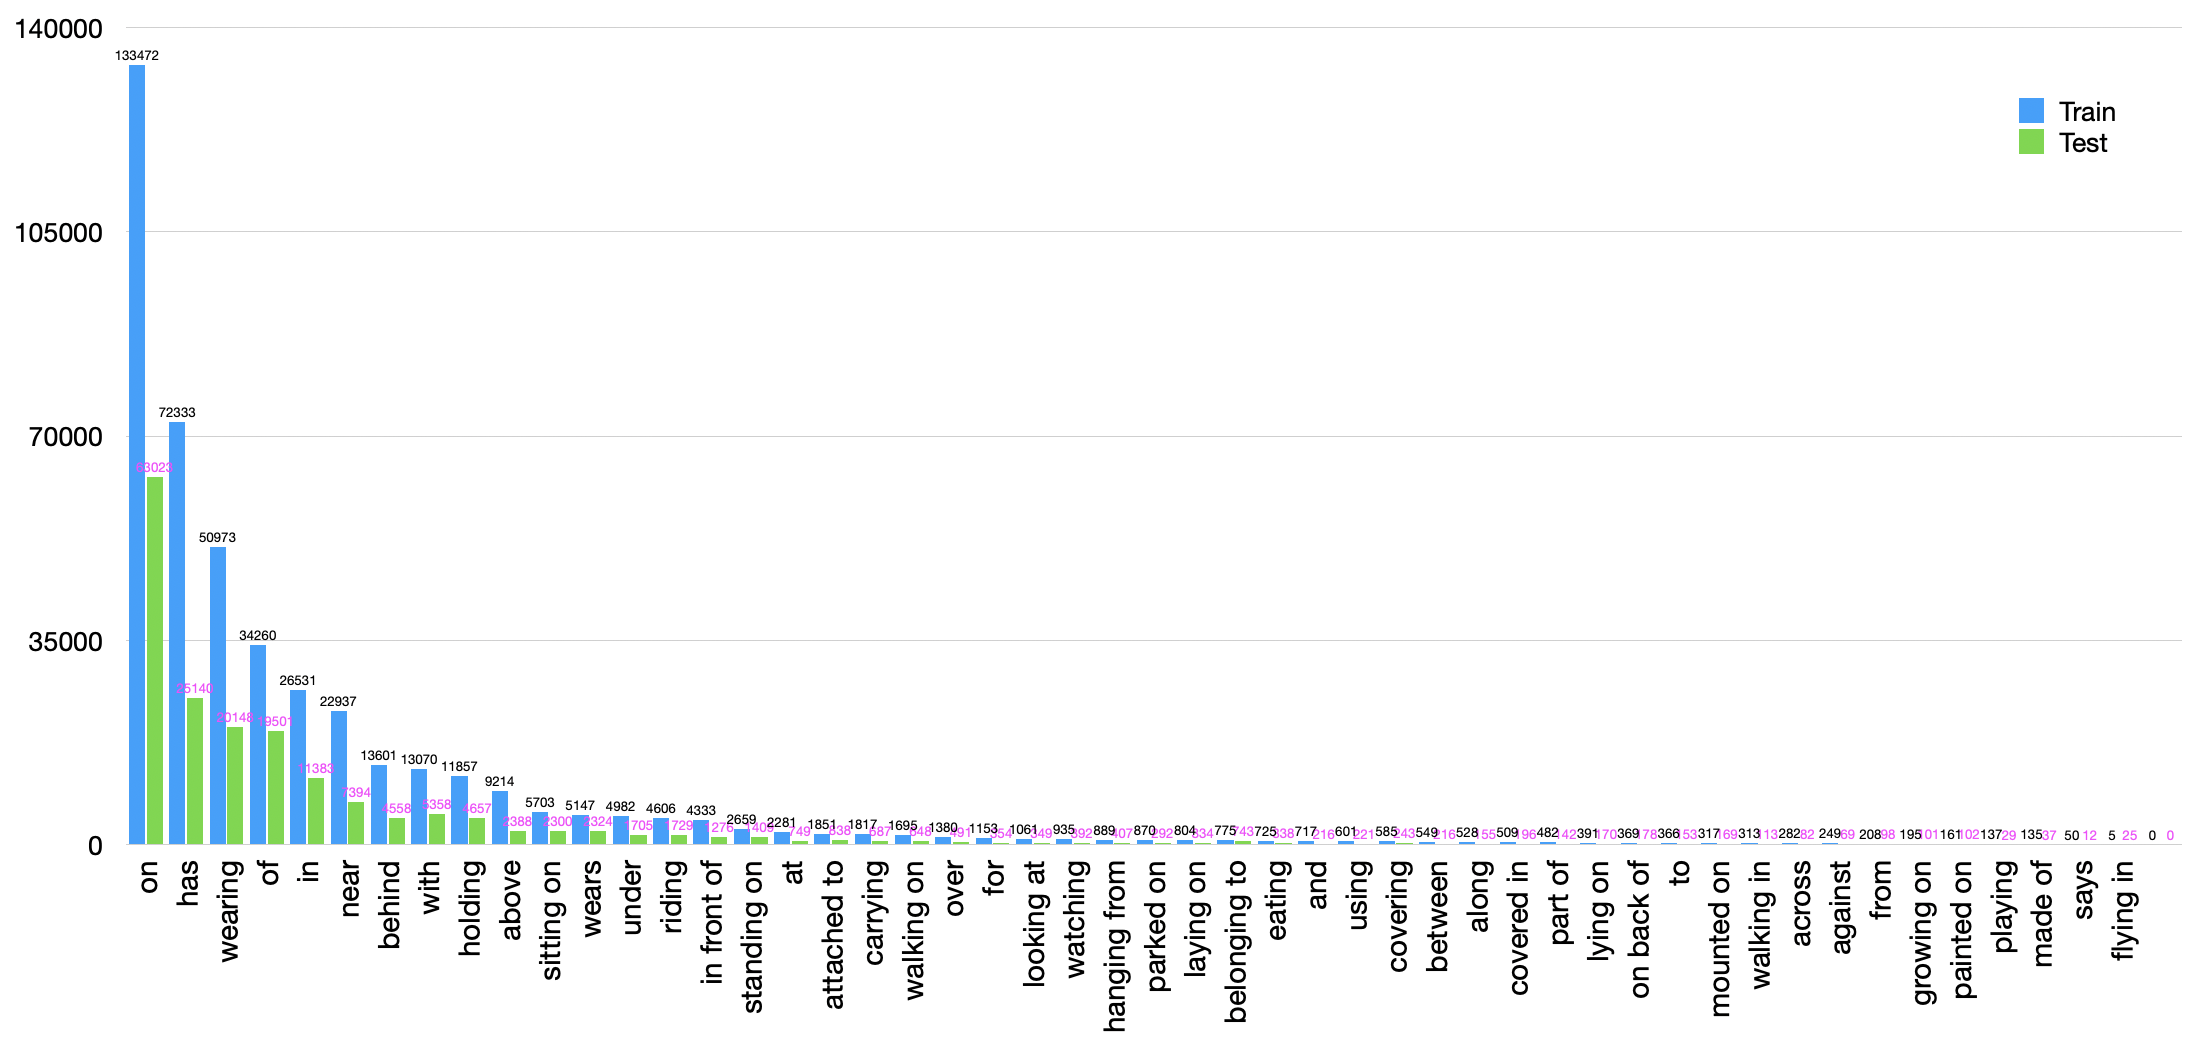
\includegraphics[width=0.9\linewidth]{figures/predicates}
	\caption[Predicate distribution of VG dataset]{Predicate distribution of VG dataset.}
	\label{fig:predicates}
\end{figure}

Figure~\ref{fig:predicates} is the predicate distribution in the data set we selected. We can conclude that the train data set and the test data set have the same predicate distribution.

\section{Evaluation Metrics}


Visual relationship detection involves object classification, localization and predicate prediction. As we mentioned before, the vrd problem has three tasks, and each task has different input information:

\begin{enumerate}[\qquad  $\bullet$]
\item Predicate Classification(\textbf{predcls}): The input is an image and a set of objects with their object classes and bounding boxes. The classes and locations of the objects are known. The model predicts the matching of subject-object pairs and their predicates.

\item Scene Graph Classification(\textbf{sgcls}): The input is an image and a set of objects with their boun- ding boxes. The classes of the objects are unknown. The model classifies the objects and predicts the matching of subject-object pairs and their predicates.

\item Scene Graph Detection(\textbf{sgdet}): The input is an image. The output involves the classes of the subjects and objects, the predicates of each subject-object pairs and the bounding boxes of each subject and object which have at least 0.5 overlap with the bounding boxes in ground truth.
\end{enumerate}

In our experiment, due to the incomplete annotation of the true relationship, we use the relationship detection $ Recall@K $ as an evaluation indicator, which measures the scores of the true relationship triples in the top K most reliable triple predictions that appear in the image.


\section{Experiments on Pixel-based Attention}
In Section~\ref{sec:pixel_base}, we put forward related ideas, through the attention map in Figure~\ref{fig:method1baseline} to find possible relationships in the detected pictures. We hope that the most relevant area can be directly reflected in the attention map, so we designed an Attention loss function(see Eq.~\ref{pixel_attention_loss}) so that the attention weights of the relevant area are higher than the non-relevant area.

We tried to add a Multihead Self-Attention module after obtaining the image feature in VGG16 based on the code of RelDN~\cite{zhang2019graphical},  so that we obtained a new image feature with a size of $ [bs, 512, 50, 66]  $and an  Attention map with a size of $ [bs, 3300, 3300] $, where bs is batch size=2. We build the baseline as the Fig.~\ref{fig:method1baseline} shown.

\subsubsection{Result of the Pixel Attention Loss  Function}
Figure~\ref{fig:motor_attention} shows the result of our training. Figure~\ref{fig:motor_img} is our input, and Figure~\ref{fig:motor_attention_map} is the corresponding attention map. In order to show it well, we normalized it and drew it through Matlab.

From the results, our attention loss has made certain modifications to the attention map. But in general, the values in the attention map are relatively average, and there is no strong distinguish ability. For instance, the ground truth pair $ <man, motorcycle>  $ shown in Fig.~\ref{fig:motor_man0}, its location of the corresponding area in attention map shown in Fig.~\ref{fig:motor_map0}. We can see the attention values in the area of the attention map(Fig.~\ref{fig:motor_attention_map}) is not higher than other areas, even be low.

In general, we use our  average of attention weights  of each pair to replace the original pair score ($ score_{pair}=score_{subject }*score_{predicate}* score_{object} $) in the evaluation to sort relation pairs, and it does not improve the recall rate of the relation.

\begin{figure}[!h]
	\centering
	\subfigure[Image input.]{
		\begin{minipage}[t]{7.5cm}
			\centering
			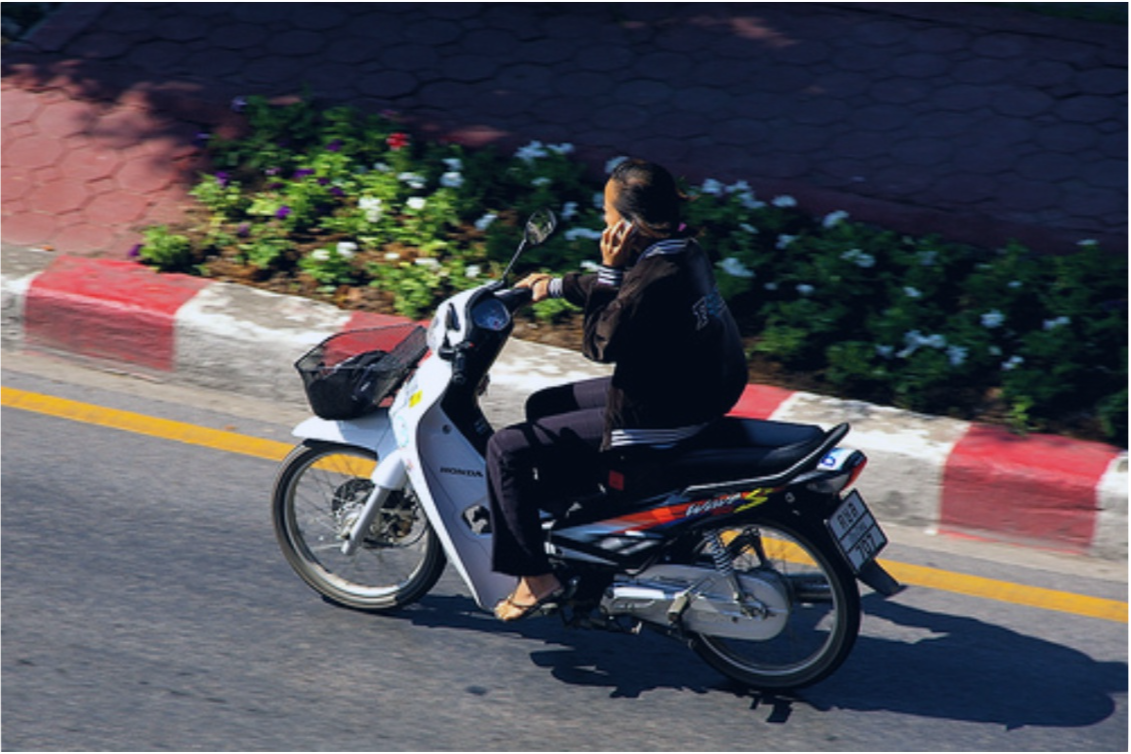
\includegraphics[width=0.95\linewidth]{figures/motor/img}
			\label{fig:motor_img}
	\end{minipage}}
	\subfigure[The result of a normalized Attention Map.]{
		\begin{minipage}[t]{7.5cm}
			\centering
			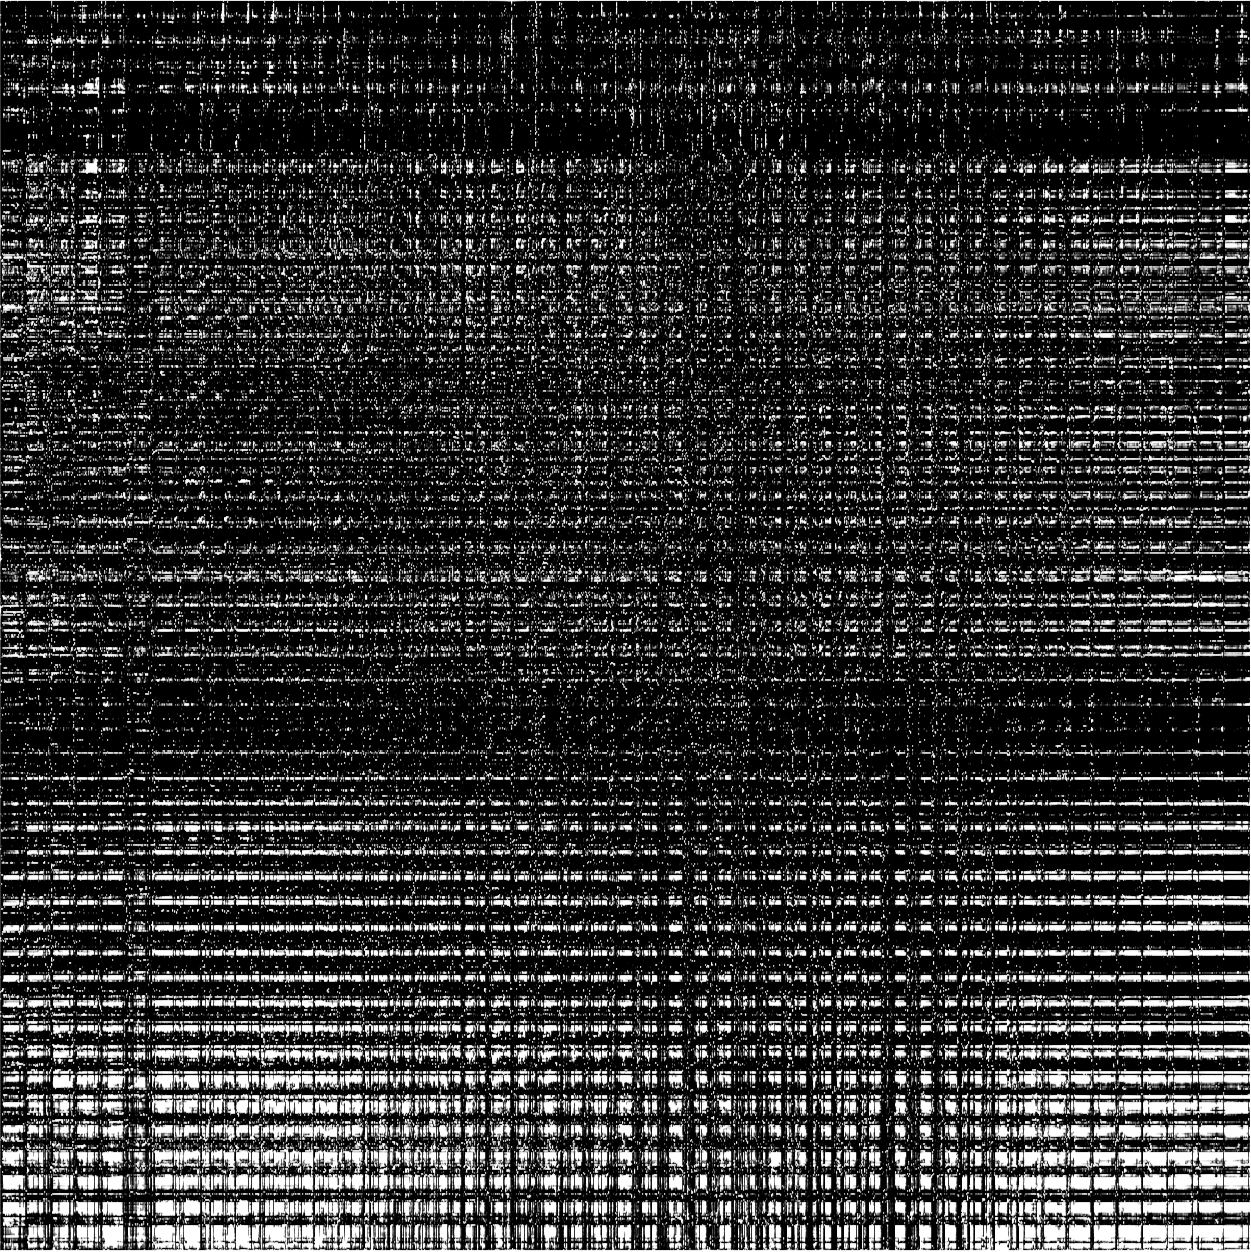
\includegraphics[width=0.95\linewidth]{figures/motor/attention}
			\label{fig:motor_attention_map}
	\end{minipage}}
	
	\caption[The result of a normalized Attention Map drawn by matlab]{The result of a normalized Attention Map drawn by matlab.}
	\label{fig:motor_attention}
\end{figure}


\subsubsection{Result analysis}

Then we analyzed the results, and we drew the position of all $ Att_{rel} $s and all $ Att_{no\_rel} $s in the attention map of image~\ref{fig:motor_img} , see Fig.~\ref{fig:overlap} $ (a) $ and $ (b) $ in the figure. And the overlap between them is shown in Figure $ (c). $ We found that $ Att_{rel }$ and $ Att_{no\_rel} $ have a very serious overlap, and are basically the same as $ Att_{rel }$, that is,  $ Att_{no\_rel} $ contains $ Att_{rel }$. The purpose of our Attention Loss is to make $ Att_{rel }$ higher and $ Att_{no\_rel }$ lower. The existence of this overlap makes its purpose very contradictory. For example, the area in Figure~\ref{fig:motor_all0} belongs to $ Att_{rel }$ but it also belongs to $ Att_{no\_rel }$ in Figure~\ref{fig:motor_all1}. We cannot make it higher and lower. This overlap in the image is shown in Figure~\ref{fig:motor_pair}. For example, for the same subject $ man $, there are  pairs $<man,ride,motorcycle>$, $ <man, \varnothing, wheel_1> $  and  $ <man, \varnothing, wheel_2>  $, their objects have an overlap, and the bounding box  of $ motor $ obviously contains the bounding box of  $ wheel $.

This overlap is not a special case. We found that almost all images have this situation, so the attention loss we designed is meaningless, and the idea of Piexl-based Attention also failed. We cannot use the attention between pixels to obtain which pair is most likely to have a relationship.

\begin{figure}[h!]
	\centering
	\subfigure[$<man,ride,motorcycle>$]{
		\begin{minipage}[t]{5cm}
			\centering
			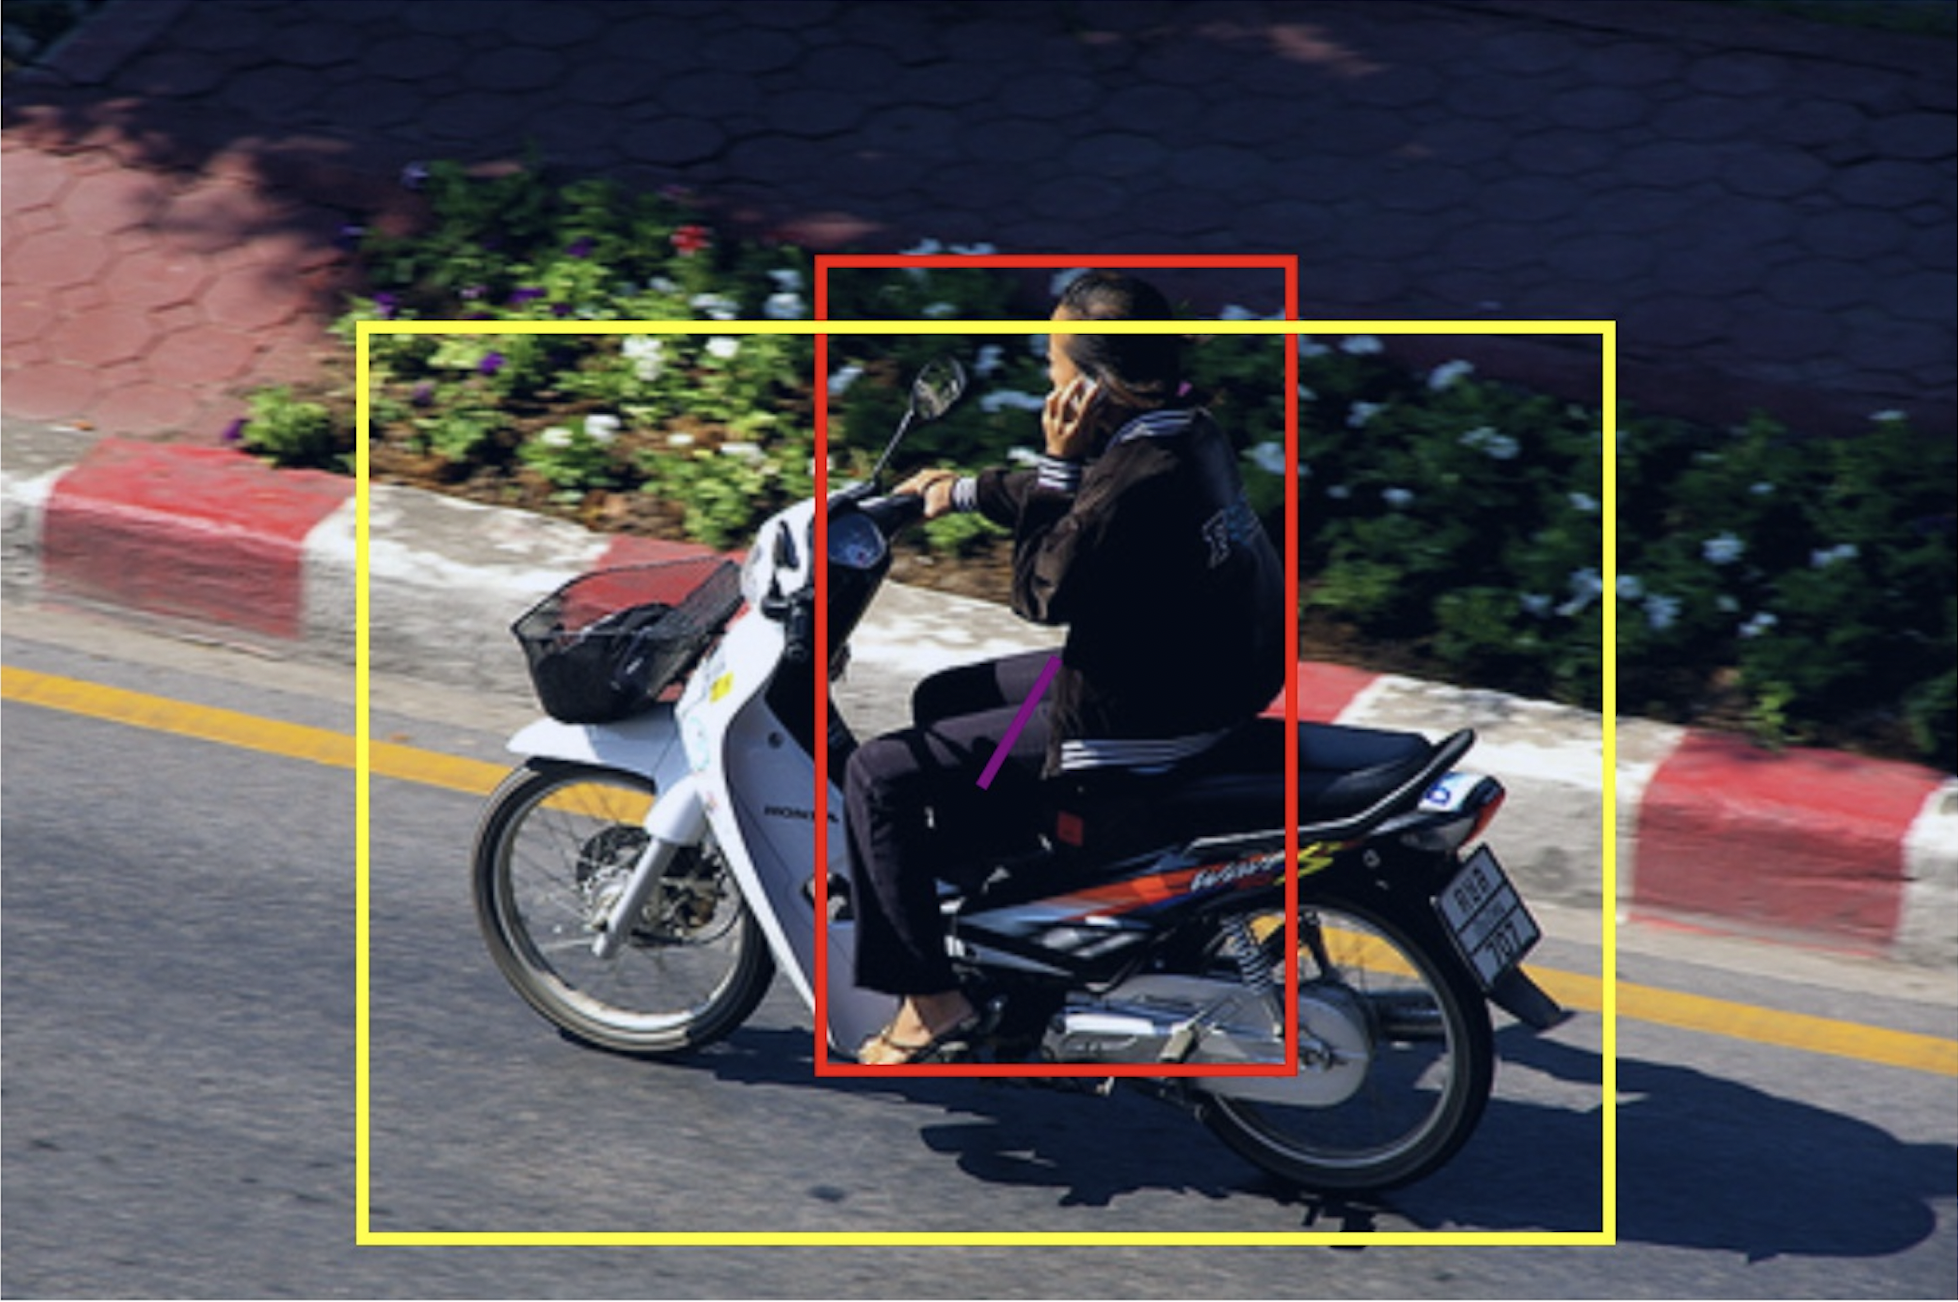
\includegraphics[width=0.9\linewidth]{figures/motor/man0}
			\label{fig:motor_man0}
	\end{minipage}}
	\subfigure[$ <man, \varnothing, wheel_1> $]{
		\begin{minipage}[t]{5cm}
			\centering
			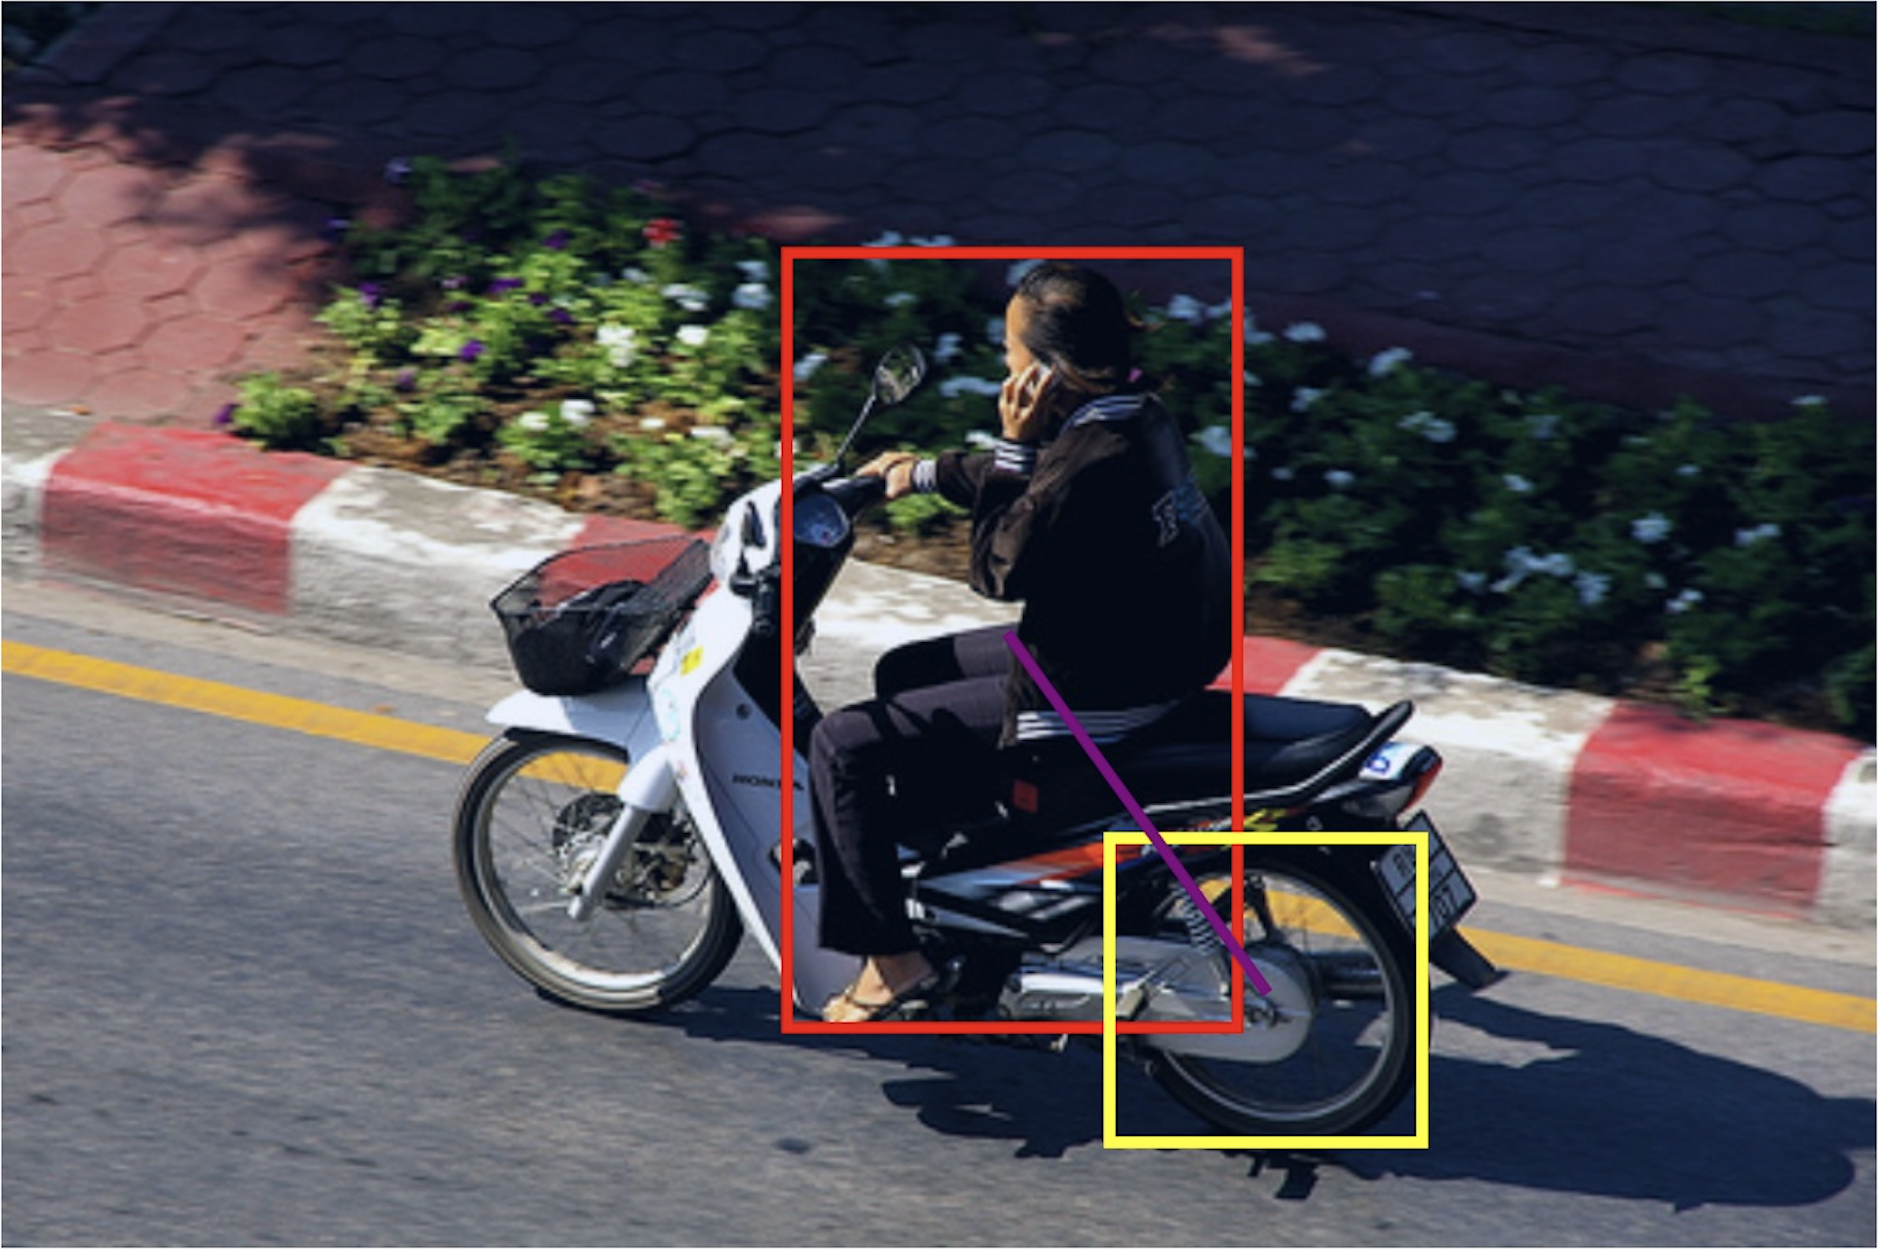
\includegraphics[width=0.9\linewidth]{figures/motor/man1}
			\label{fig:motor_map0}
	\end{minipage}}
	\subfigure[$ <man, \varnothing, wheel_2>  $]{
		\begin{minipage}[t]{5cm}
			\centering
			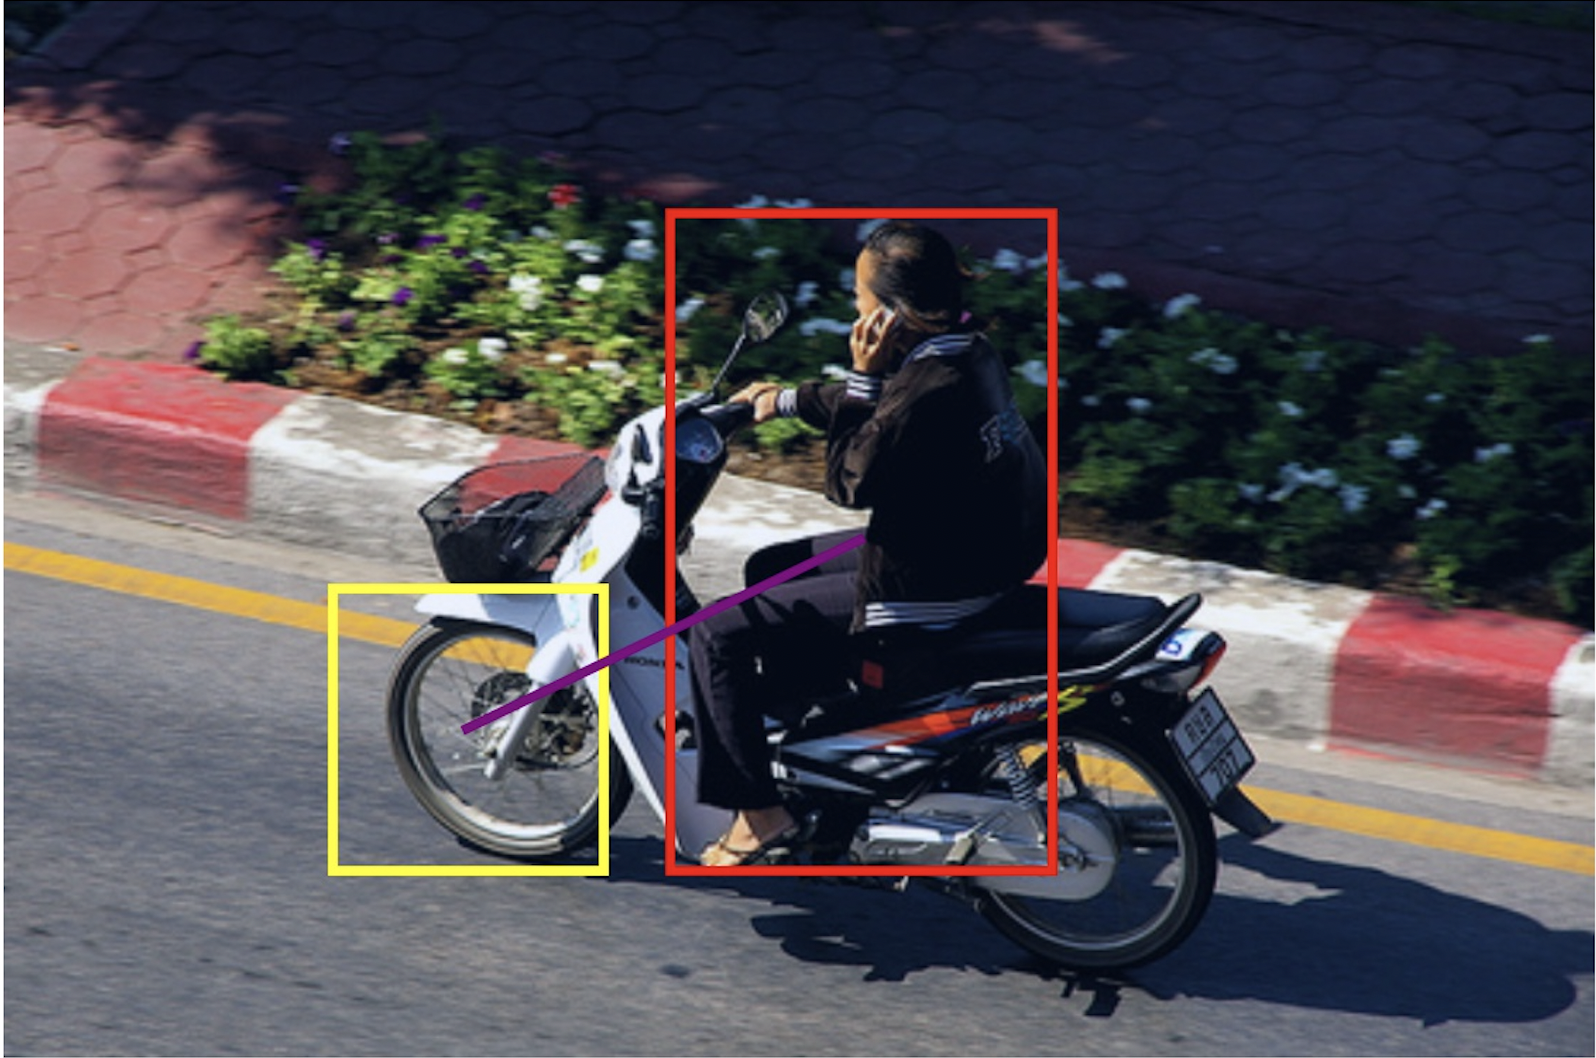
\includegraphics[width=0.9\linewidth]{figures/motor/man2}
			\label{fig:motor_man1}
	\end{minipage}}

	\subfigure[$Attention_{man \to motorcycle} $]{
		\begin{minipage}[t]{5cm}
			\centering
			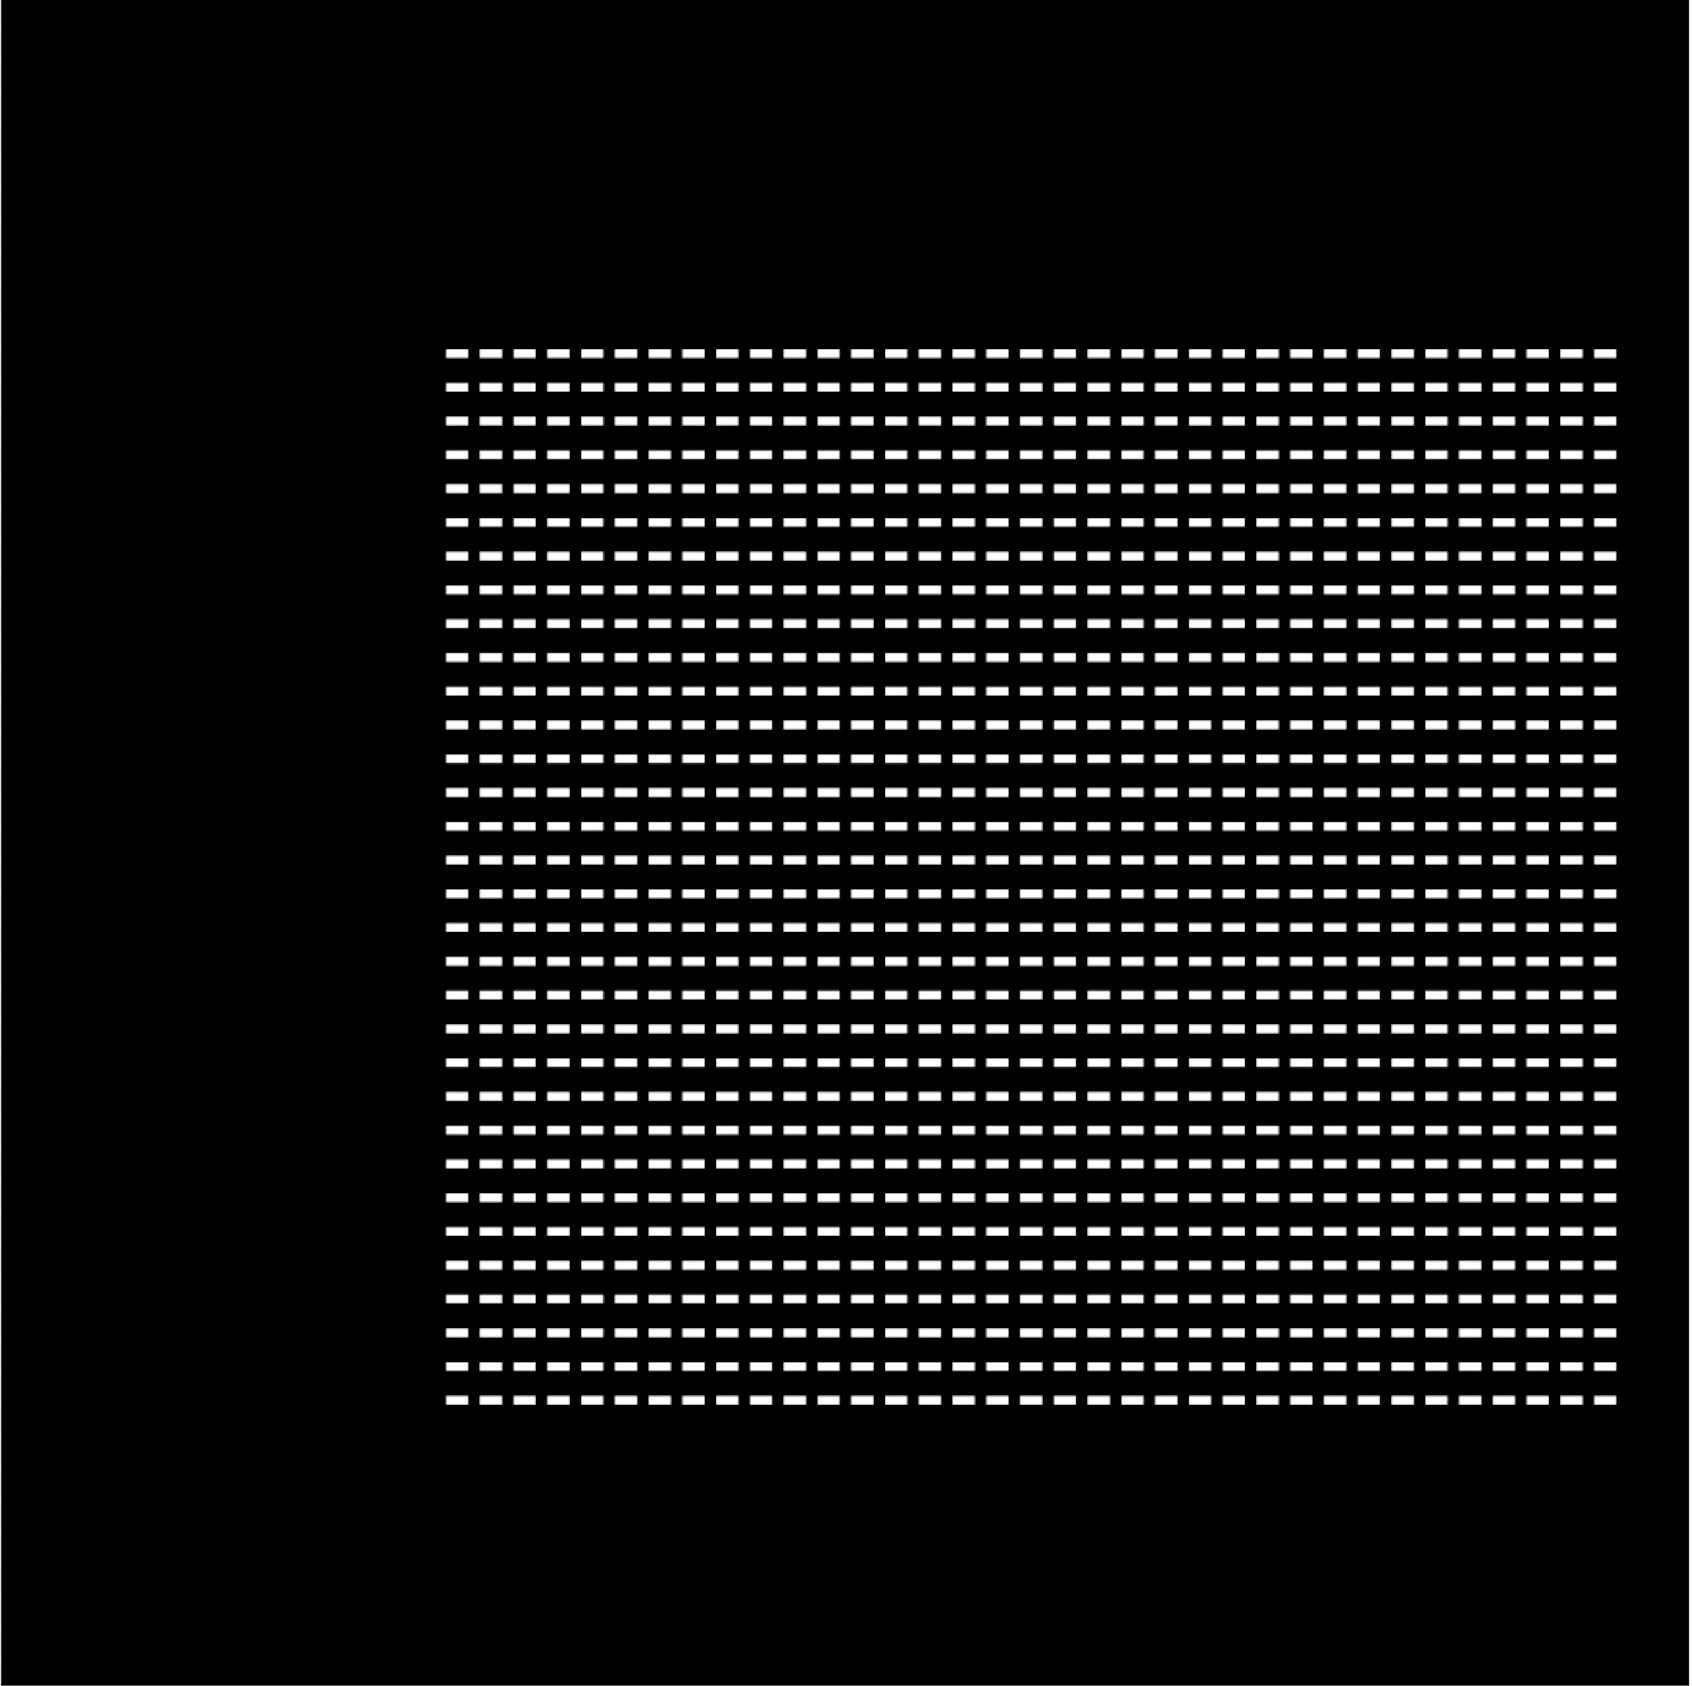
\includegraphics[width=0.9\linewidth]{figures/motor/map0}
			\label{fig:motor_map1}
	\end{minipage}}
	\subfigure[$Attention_{man \to wheel_1} $]{
		\begin{minipage}[t]{5cm}
			\centering
			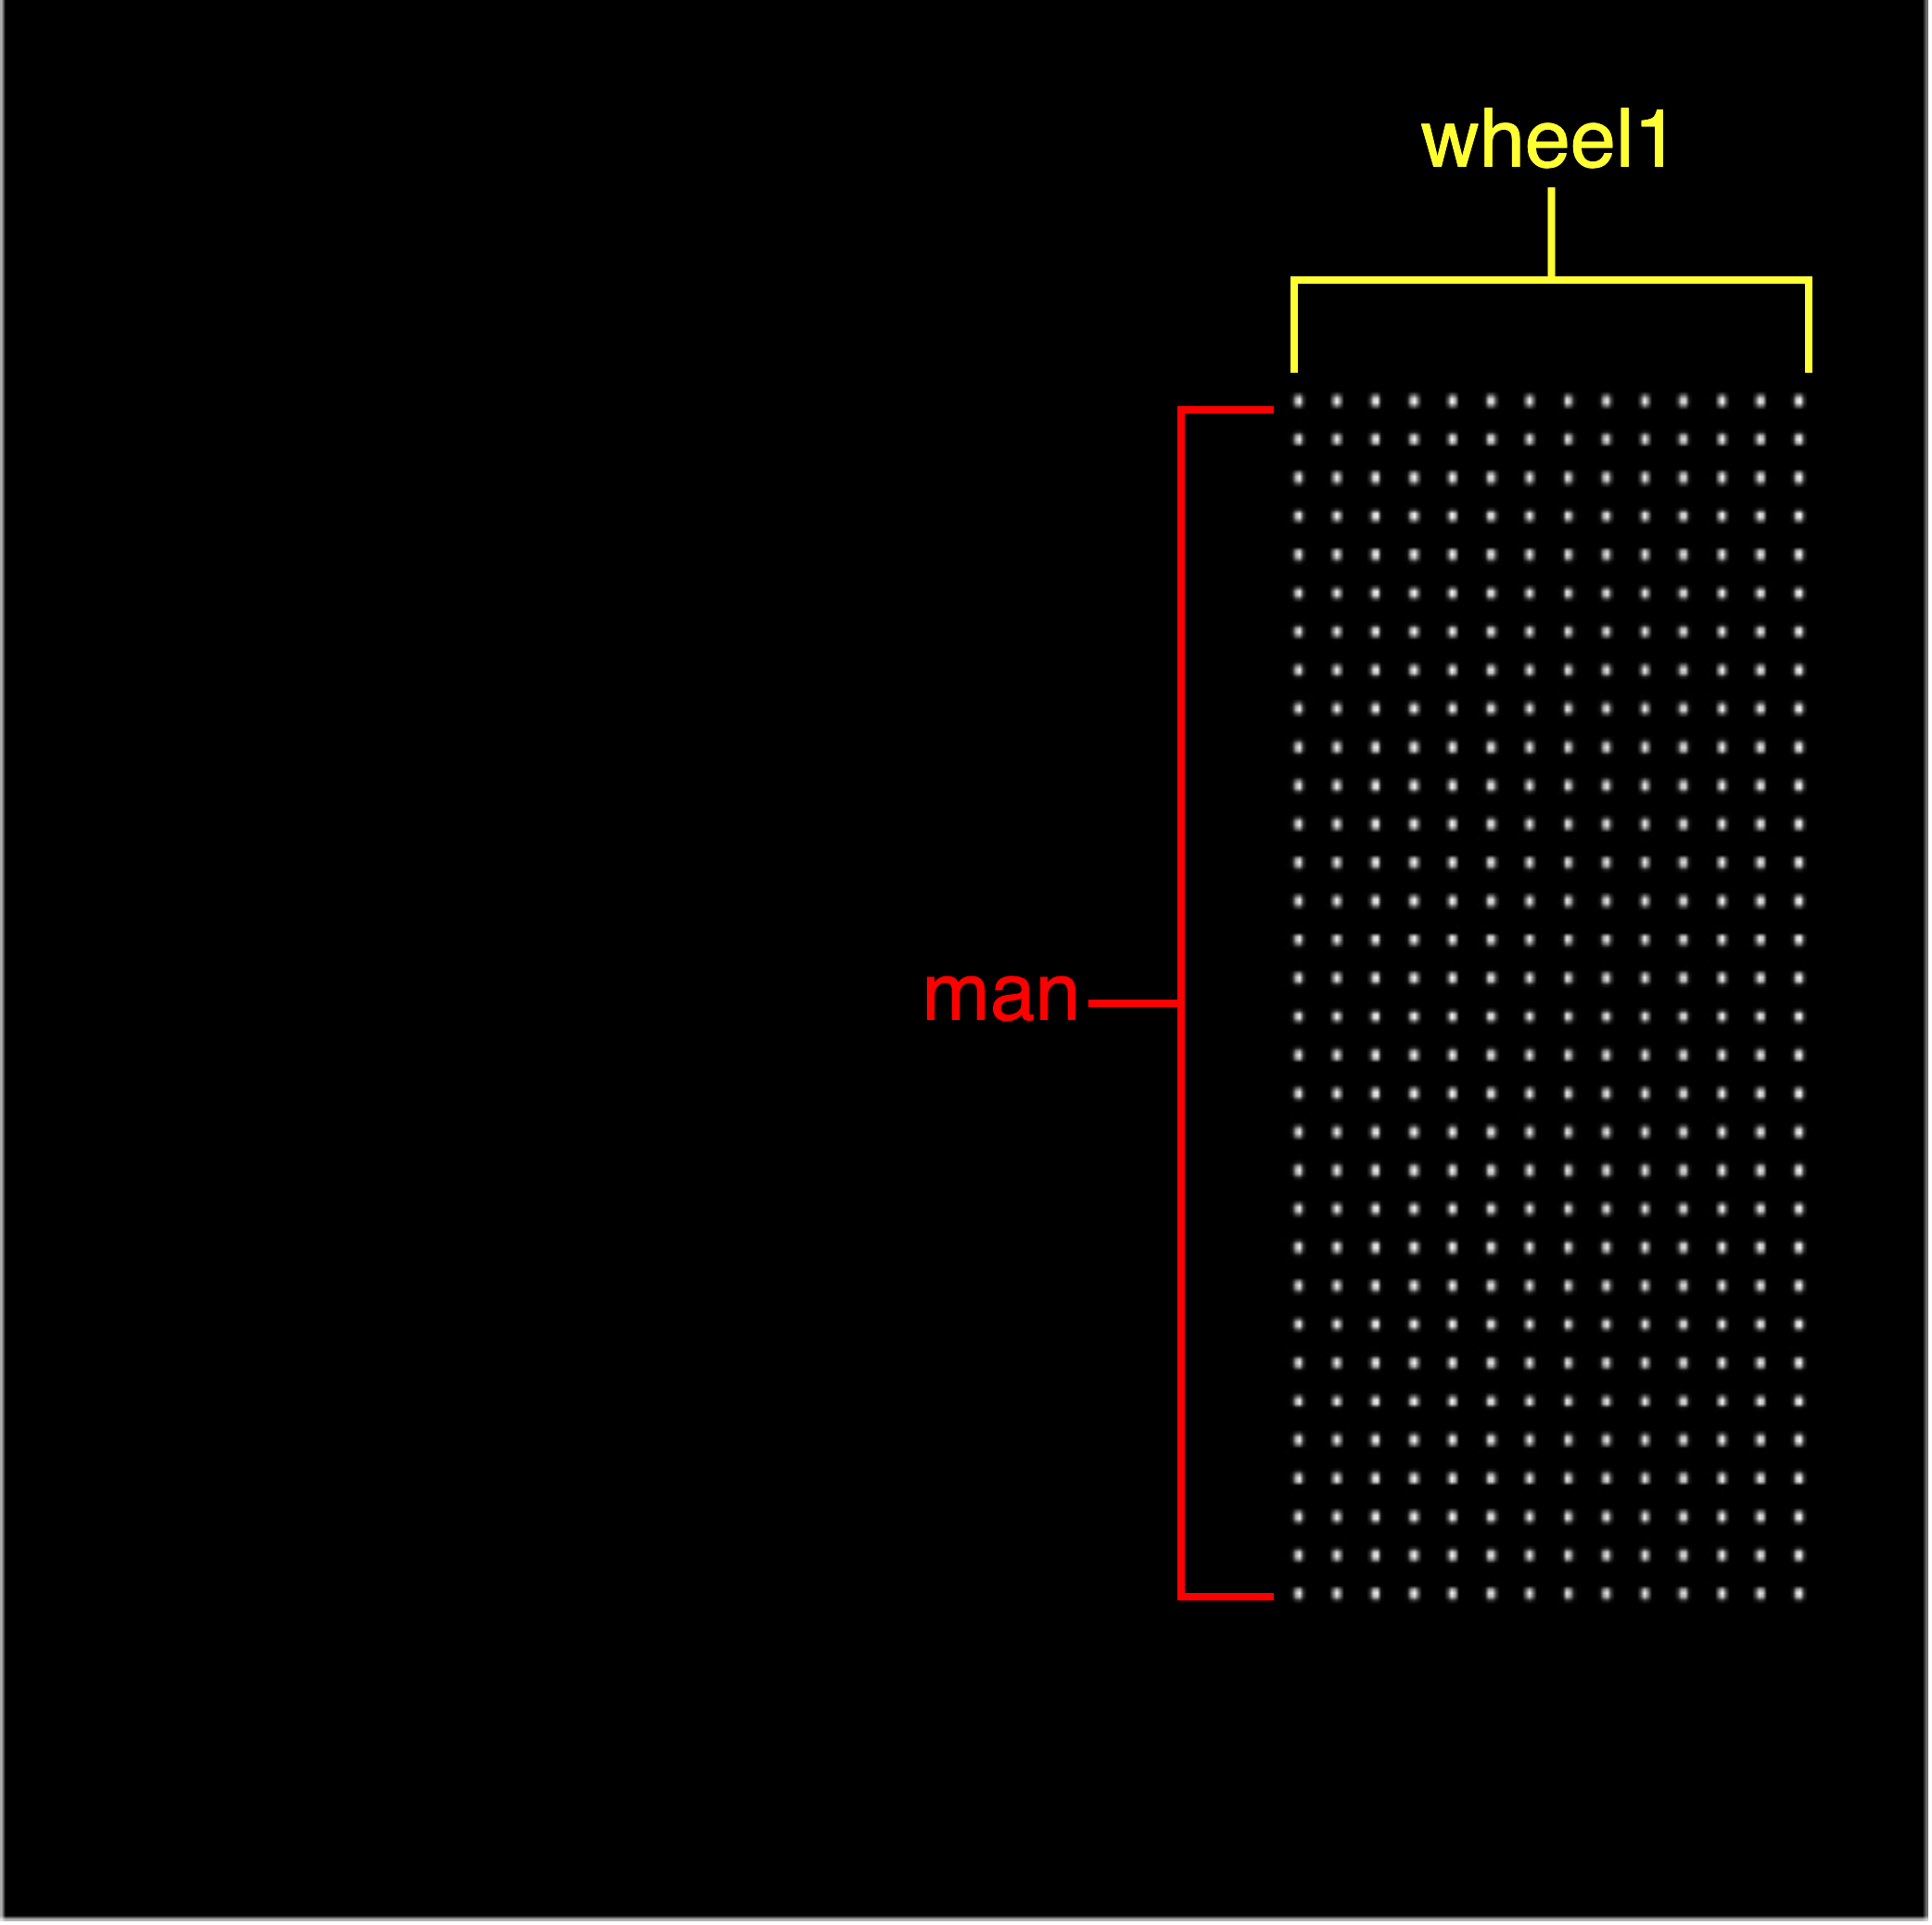
\includegraphics[width=0.9\linewidth]{figures/motor/map1}
			\label{fig:motor_man2}
	\end{minipage}}
	\subfigure[$Attention_{man \to wheel_2} $]{
		\begin{minipage}[t]{5cm}
			\centering
			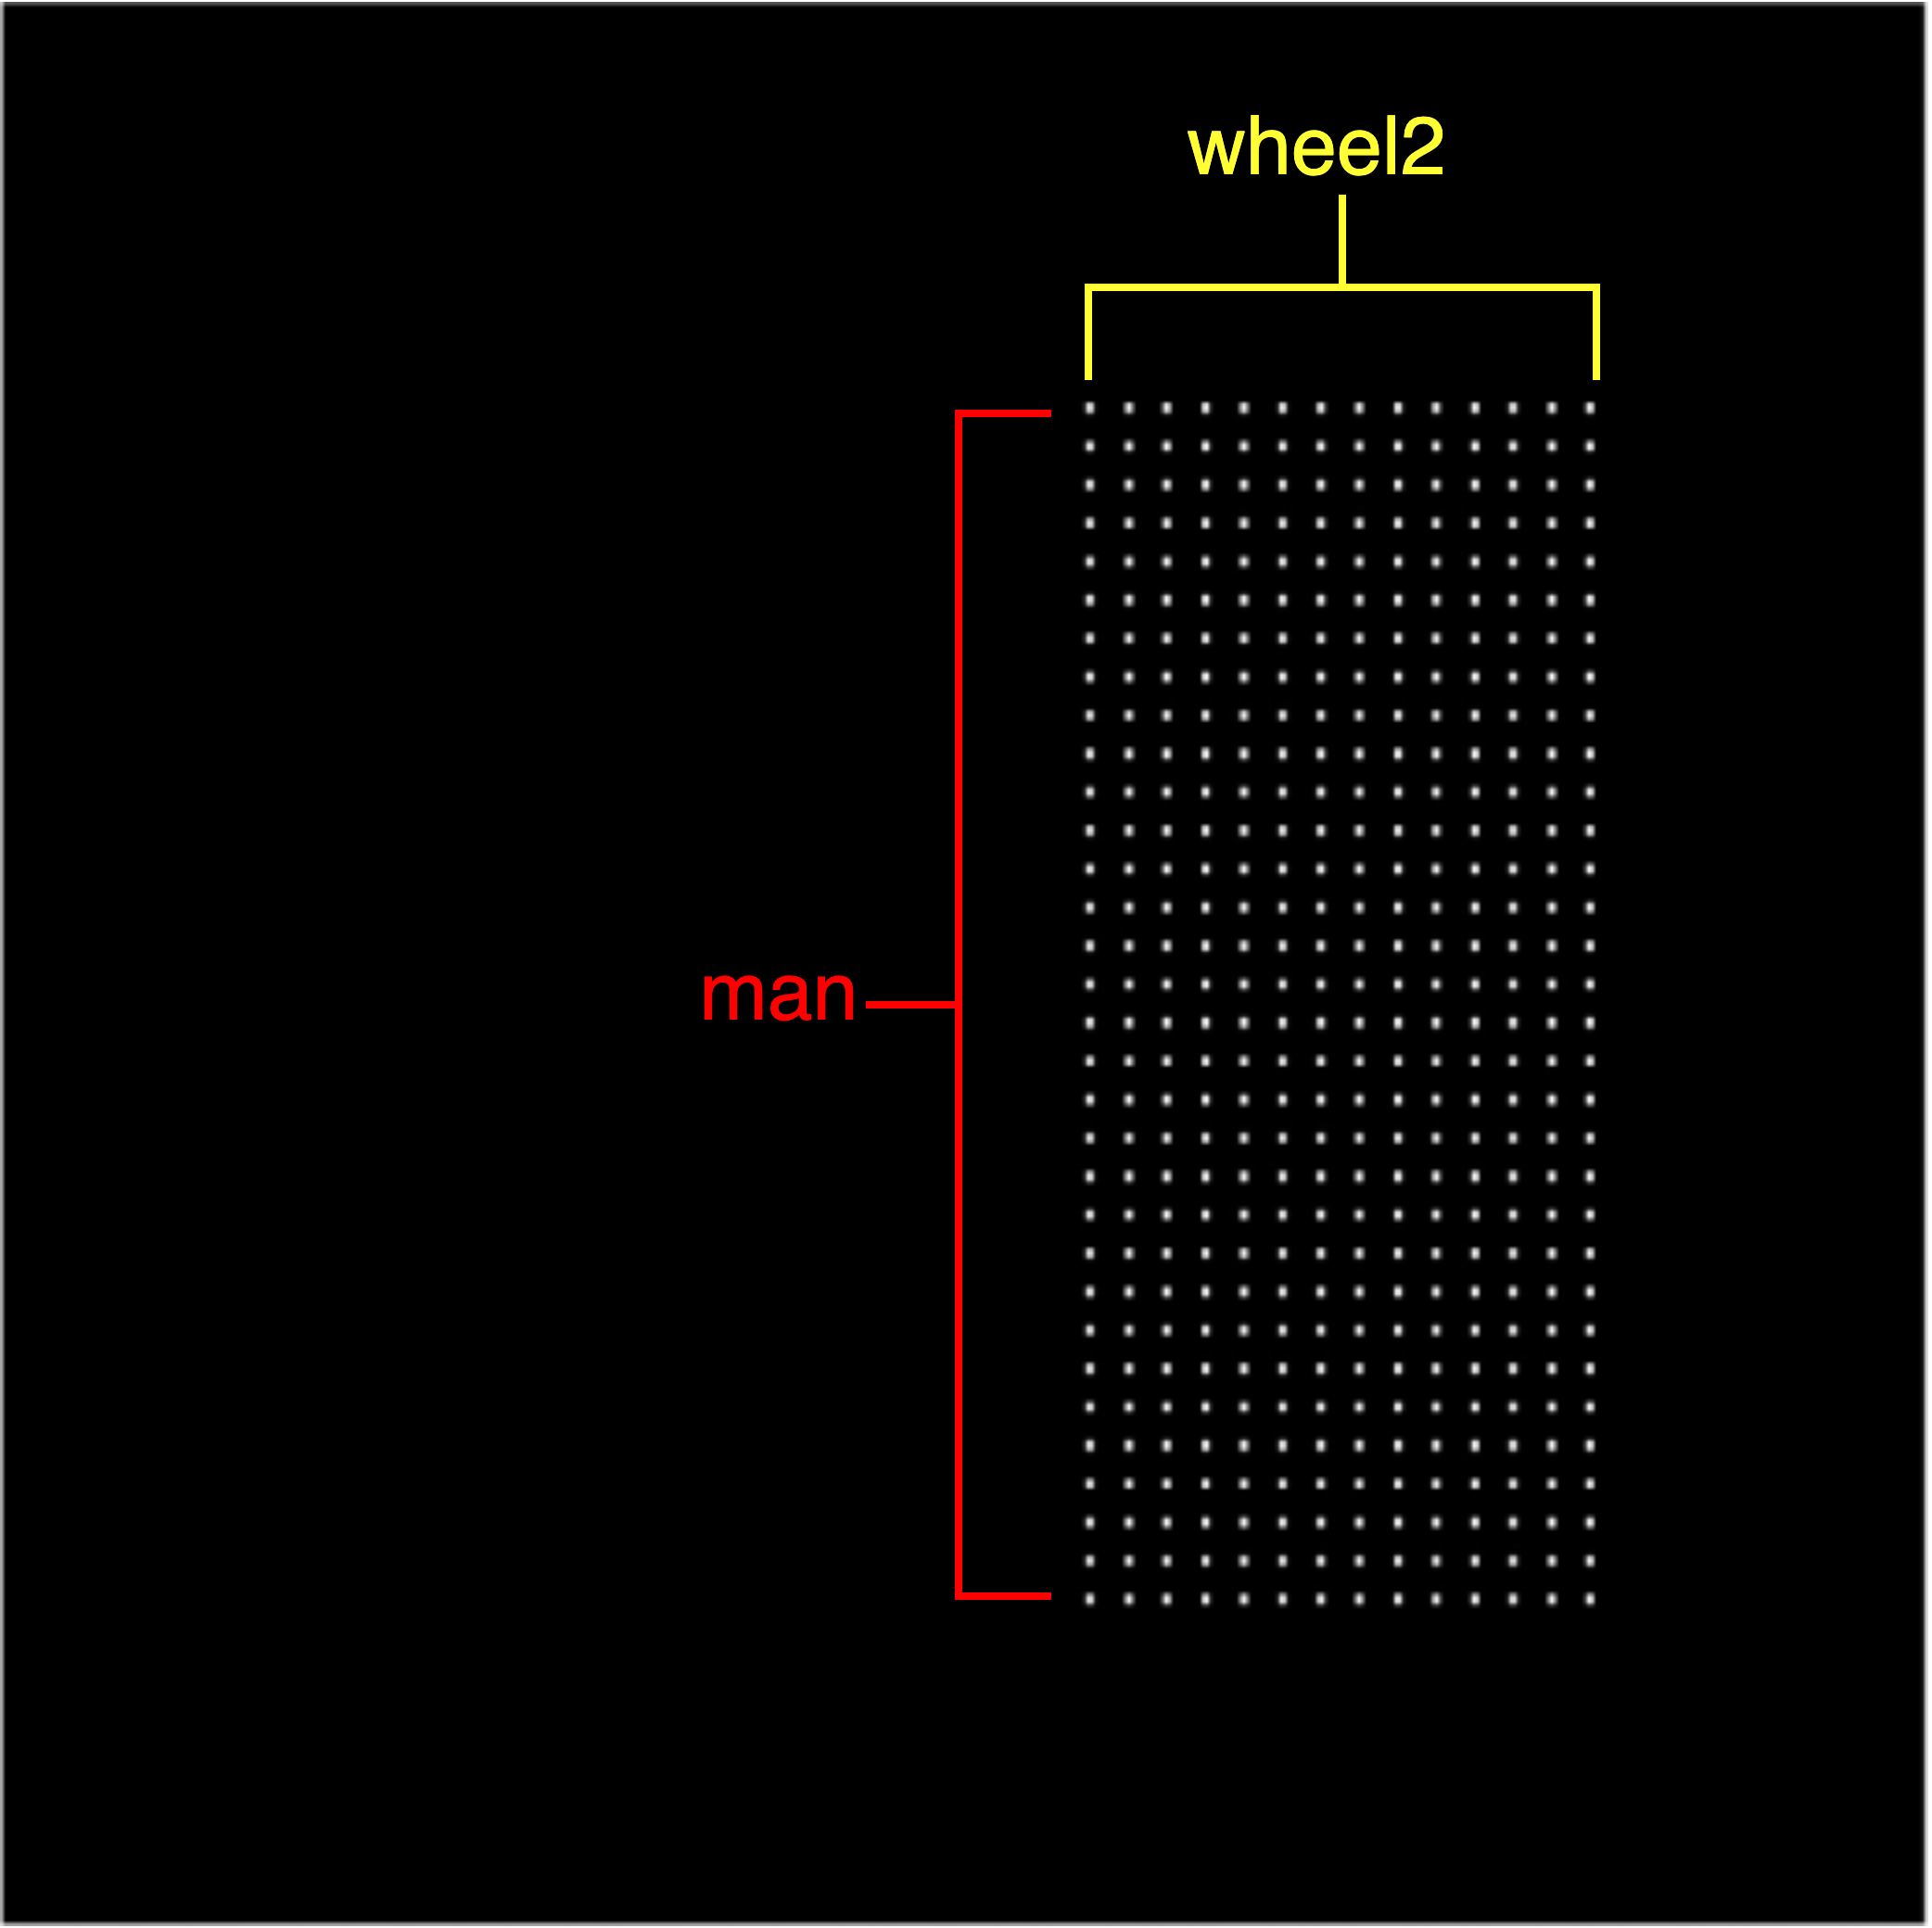
\includegraphics[width=0.9\linewidth]{figures/motor/map2}
			\label{fig:motor_map2}
	\end{minipage}}
	
	\caption[The attention map of each pair.]{The attention map of each pair, where $ (a) $ is the ground truth pair and $ (d) $ is its corresponding position in the attention map. $ (b) $, $(c) $ are no relationship pair, and $ (e) $, $ (f) $ is theirs corresponding positions in the attention map.}
	\label{fig:motor_pair}
\end{figure}

\begin{figure}[tbph!]
	\centering
	\subfigure[All pixels of $Att_{rel}$]{
		\begin{minipage}[t]{5cm}
			\centering
			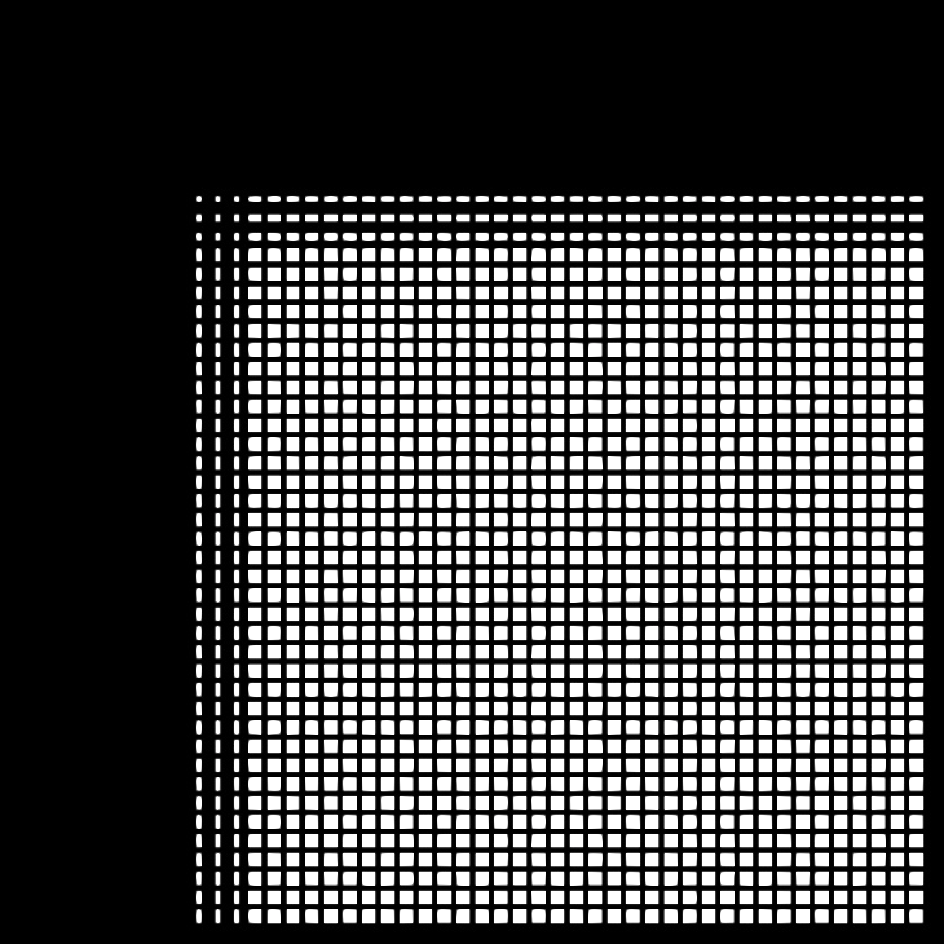
\includegraphics[width=0.9\linewidth]{figures/motor/all0}
			\label{fig:motor_all0}
	\end{minipage}}
	\subfigure[All pixels of $ Att_{no\_rel }$]{
		\begin{minipage}[t]{5cm}
			\centering
			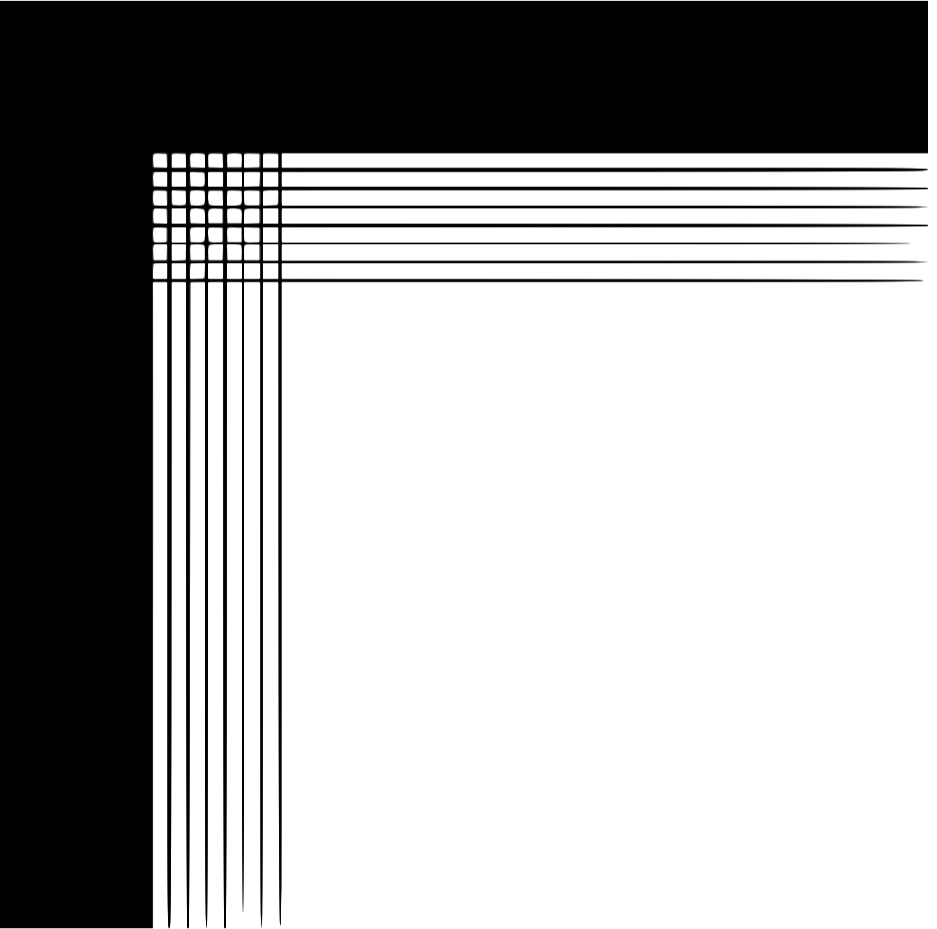
\includegraphics[width=0.9\linewidth]{figures/motor/all1}
			\label{fig:motor_all1}
	\end{minipage}}
	\subfigure[Overlap]{
		\begin{minipage}[t]{5cm}
			\centering
			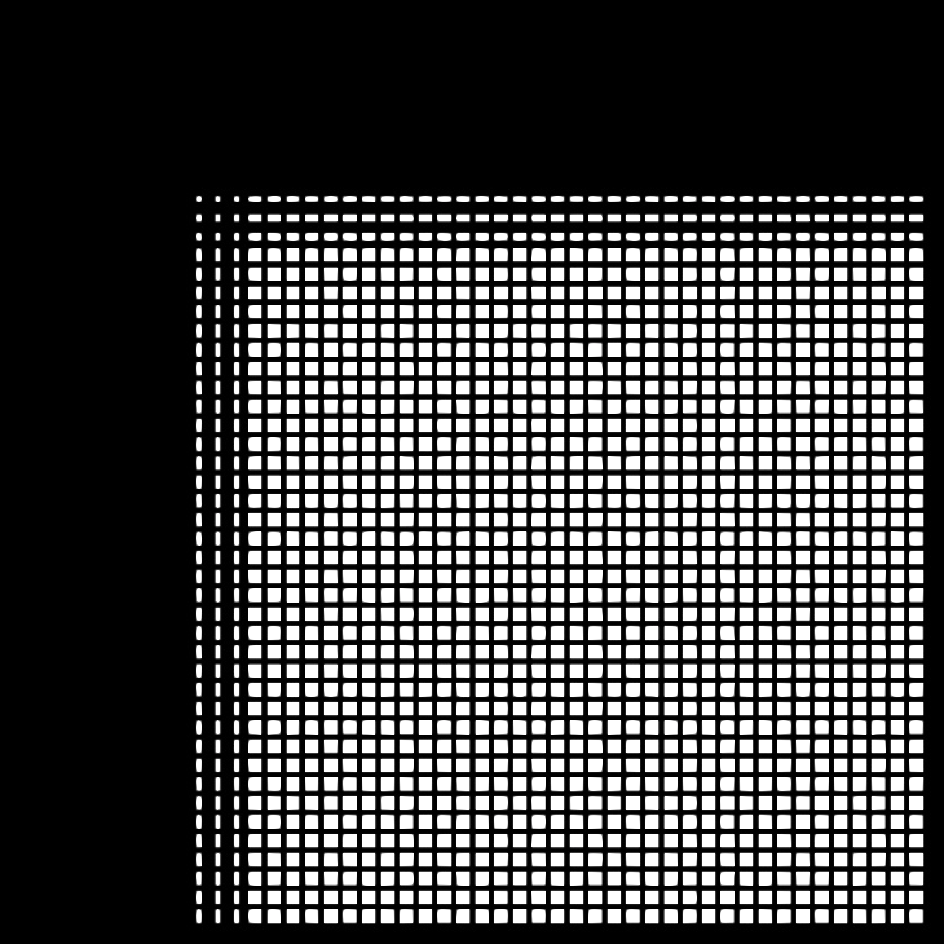
\includegraphics[width=0.9\linewidth]{figures/motor/all0}
			\label{fig:motor_all2}
	\end{minipage}}
	
	\caption[The overlap in Attention map]{The overlap in Attention map.}
	\label{fig:overlap}
\end{figure}



\section{Experiments on Proposed Framework}

As mentioned above, our Pixel Attention idea did not meet our expectations due to the overlap. In this section, we introduce in detail the relevant experiments and results of our Retina Net.

\subsection{Implementation details}
We have implemented our model in $ pythorch\-0.4 $~\cite{paszke2019pytorch}. The input of our model is the same as~\cite{zellers2018neural} , that is an image with a size of $ 592 \times 592 $. We have used VGG16~\cite{simonyan2015deep} backbone pretrained on visual genome dataset. As mentioned in our Sec.~\ref{sec:retinanet}, the encoder and the two decoder modules accept input features of size 2048. We have used 3x Encoder, 3x Object Decoder , 3x Relation Decoder and 8 attention head for transformer network. The glove vector embedding has size 200. SGD with momentum along with learning rate of $ 10^{-3 }$ and our batch size is 6. Also, we have used cross-entropy loss for both of our object and relation classification loss.

We have followed the same evaluation as in current benchmark of motifsNet~\cite{zellers2018neural} and computed and predicate classification (PREDCLS), scene graph classification (SGCLS) and scene graph generation(SSG).For the task SSG, we use a learnable object query, and use the Hungarian matching algorithm to match each object feature. For the other two tasks, we use our custom object query to obtain the object feature.


\subsection{Experiment on Object query}

We will discuss the feasibility of our proposed object query to replace learnable query. The task PredClS has classes and bounding boxes information, so we designed several object queries based on the known information, as shown in Fig.~\ref{fig:objectquery}, Fig.~\ref{fig:objquery1} and Fig.~\ref{fig:objquery2}. We call them  \textit{objec query 1} ,  \textit{objec query 2} , and  \textit{objec query 3}  respectively. We will discuss their pros and cons, and their substitutability.

We have already mentioned object query 1 above, it has the spatial information of the entity, while the object query 2 is to add a class word embedding on his basis, so that our object query has semantic information. For the object query 3, we only made a simple design. The bounding box of each entity in a picture is different, so their object query is also different.

\begin{figure}[tbph!]
	\centering
	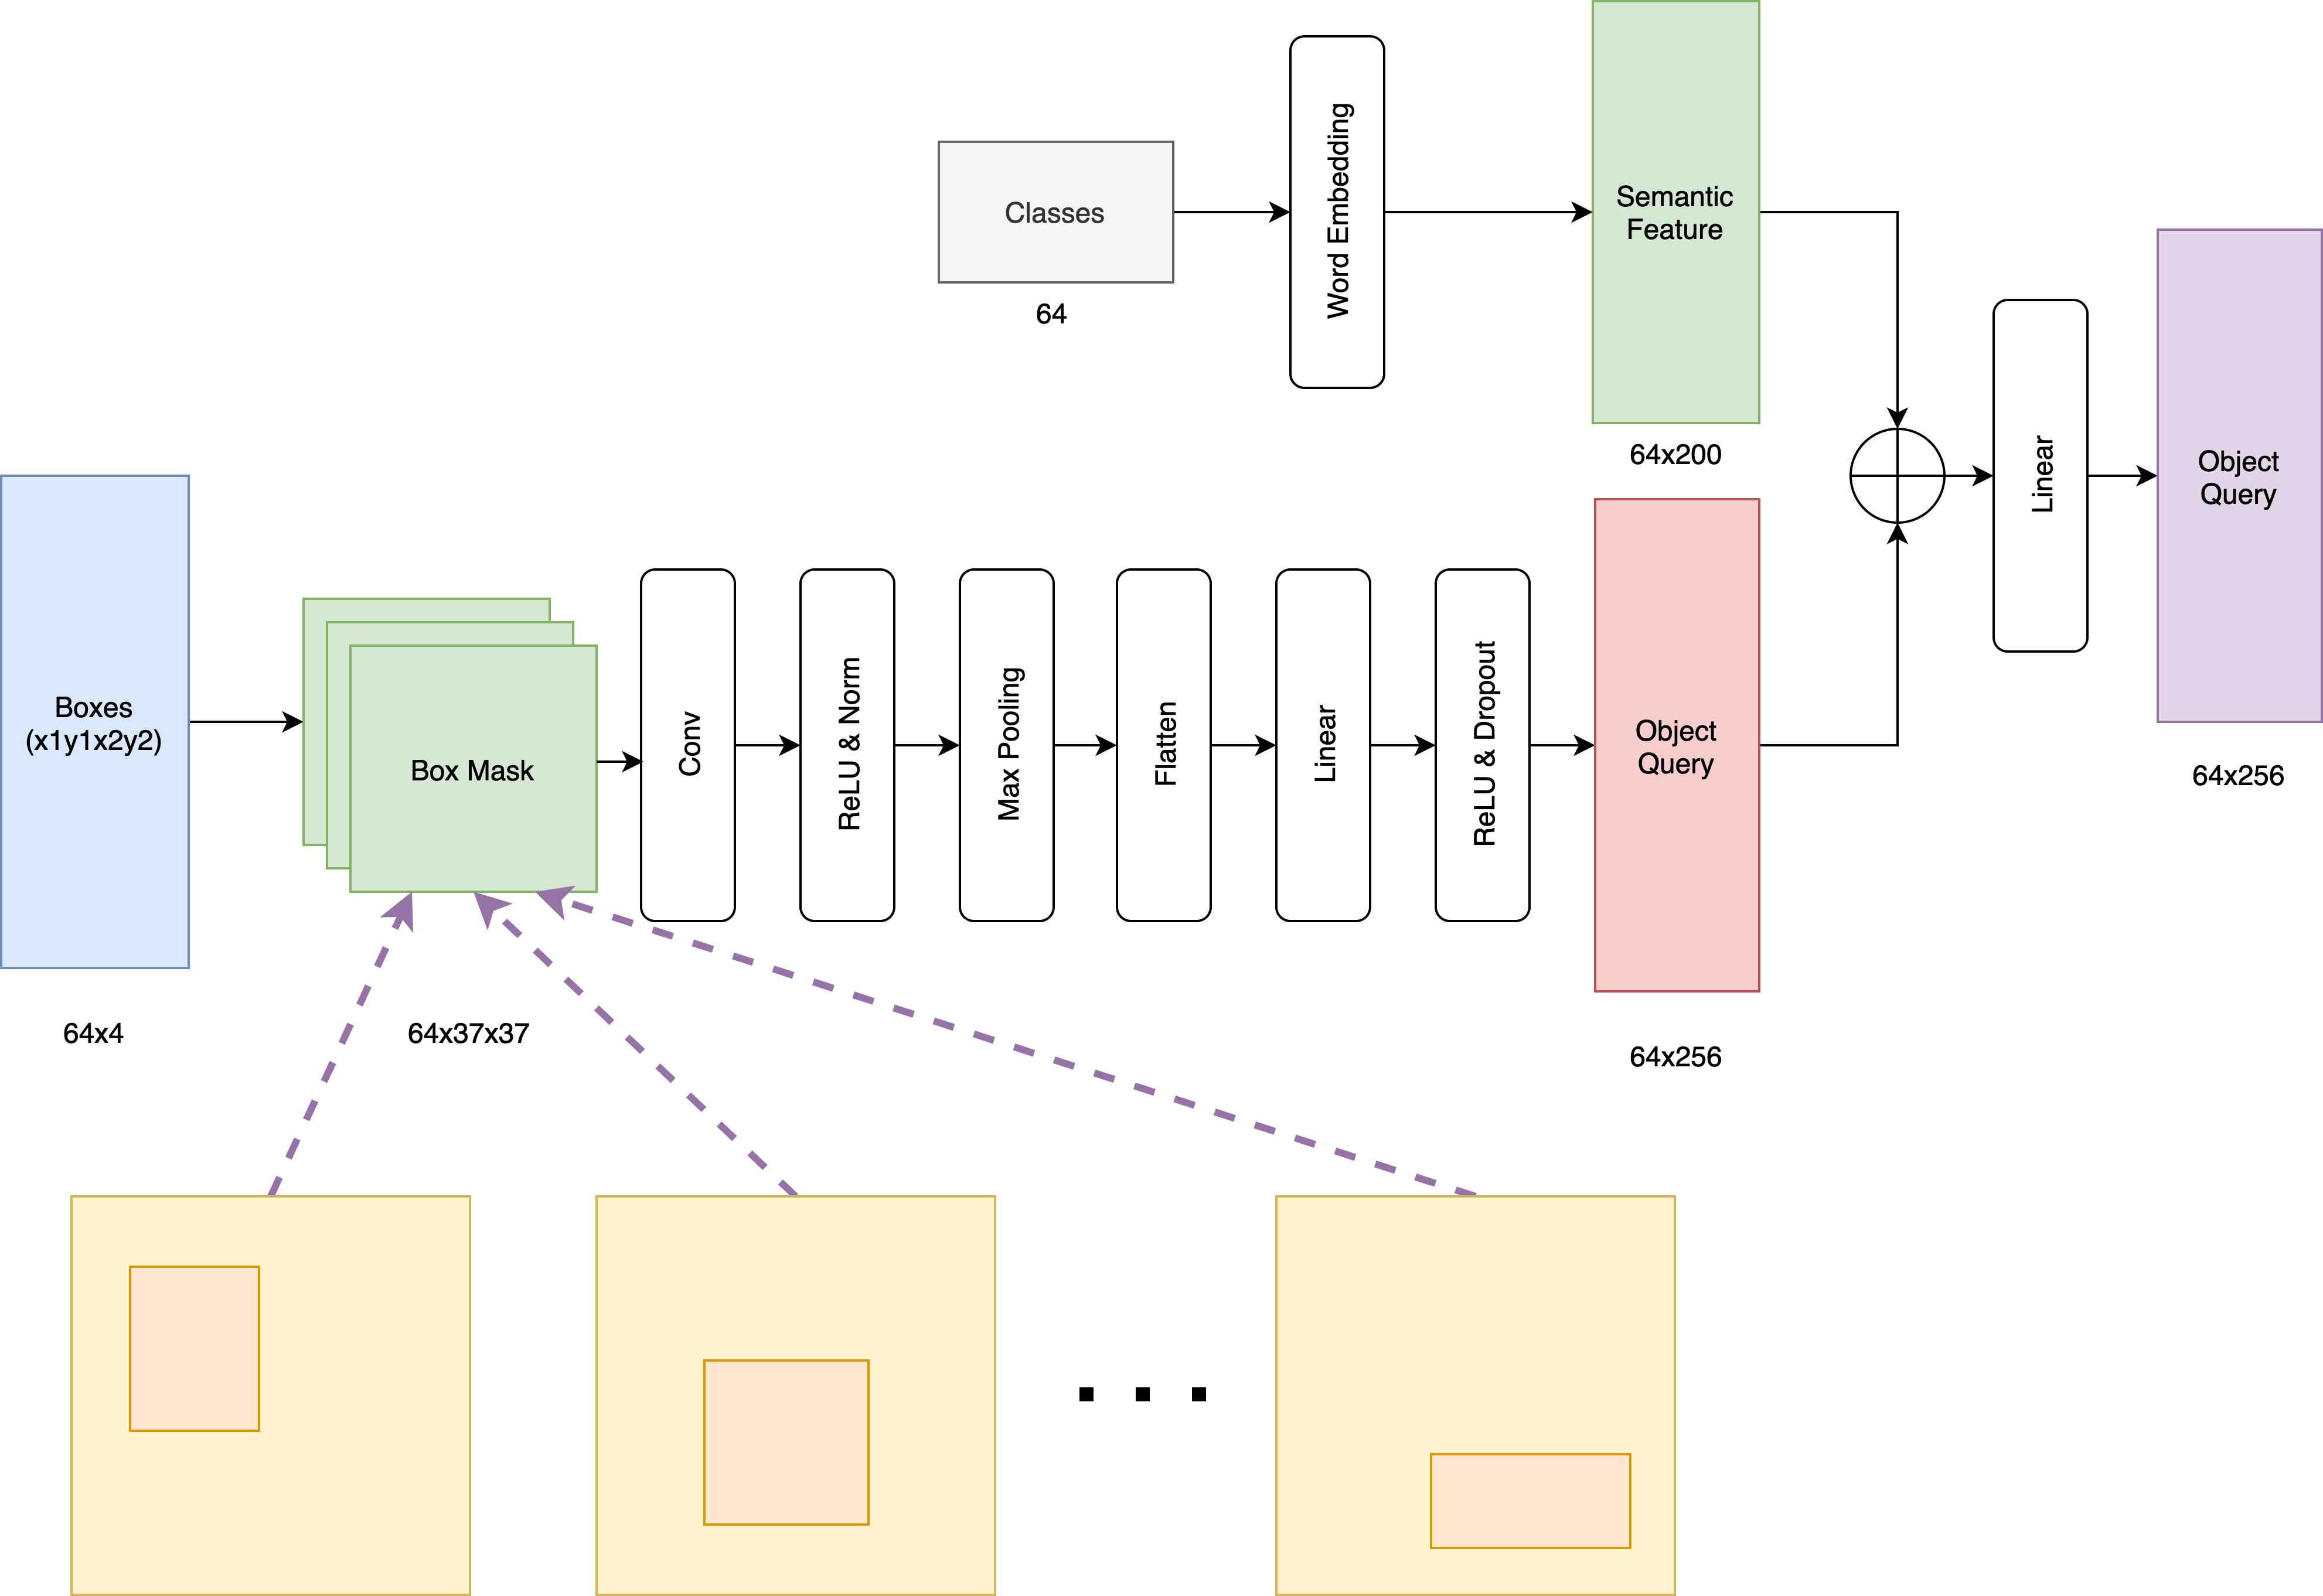
\includegraphics[width=0.9\linewidth]{figures/obj_query1}
	\caption[Illutrastion of the object query 2]{Illutrastion of the object query 2. Compared with object query1, we integrate the semantic feature of objects.}
	\label{fig:objquery1}
\end{figure}

\begin{figure}[tbph!]
	\centering
	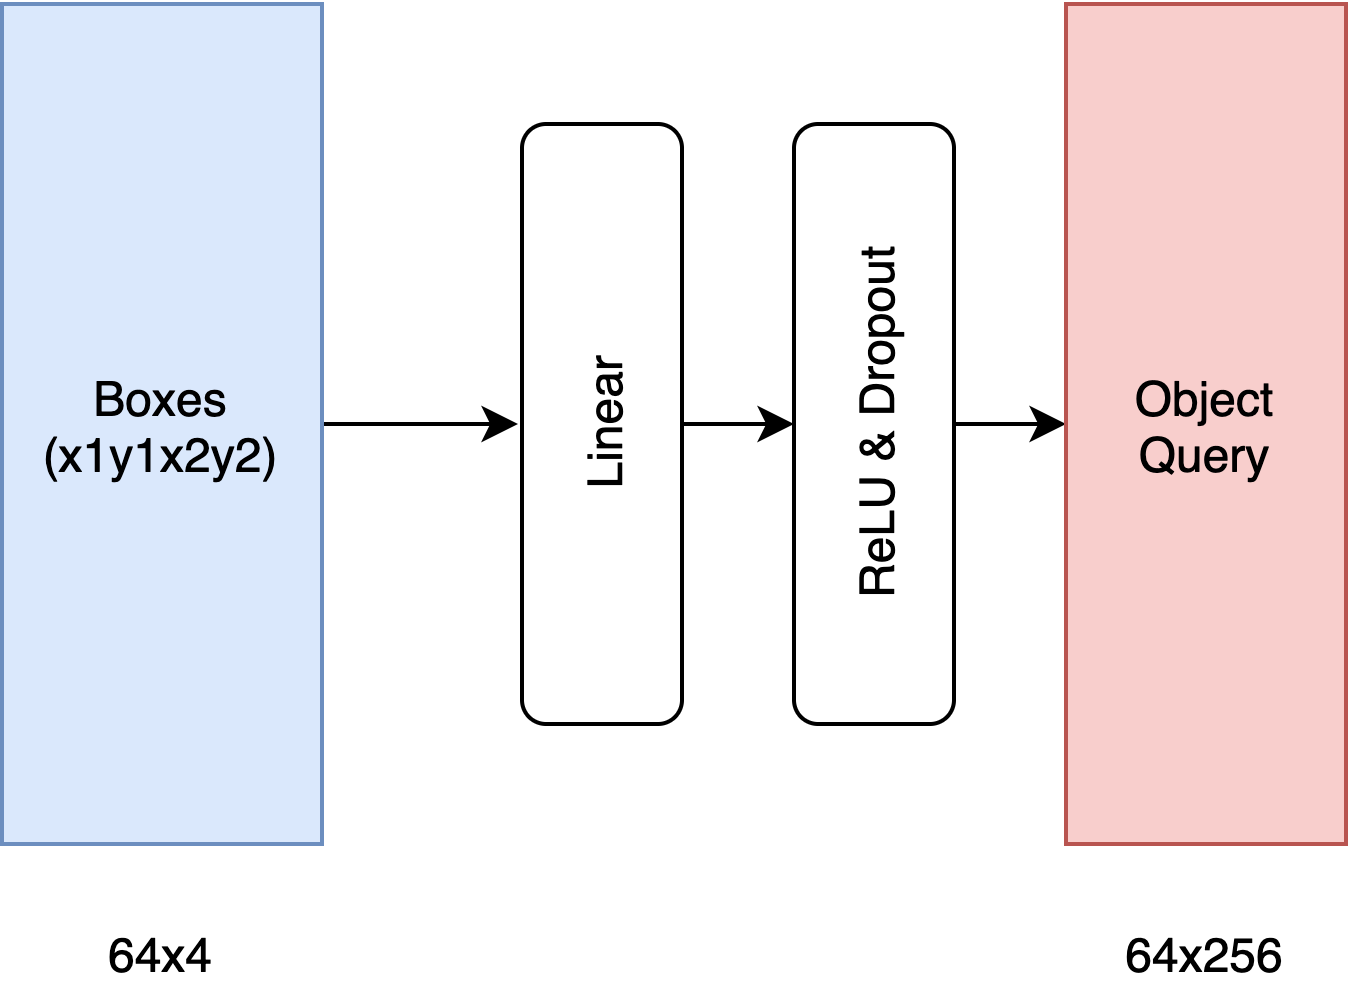
\includegraphics[width=0.5\linewidth]{figures/obj_query2}
	\caption[Illutrastion of the object query 3]{Illutrastion of the object query 3,we only added a simple linear layer behind the bounding box.}
	\label{fig:objquery2}
\end{figure}

\subsubsection{Correspondence of the Object Query }

When people use a learnable embedding vector as the query, such as detr, they need to use the Hungarian matching algorithm to find the most matching object feature, because their query has no actual physical meaning. And our object query contains relevant information of each object, such as spatial information and semantic information. He is in one-to-one correspondence with the entities in the picture.

In order to verify the correspondence between our object query and the entity in the picture, we designed a regression experiment: we add an Multilayer Perceptron(MLP) module after ours object query and object feaure, then observe whether they can regain the spatial information of the object. We use IoU and GIoU~\cite{rezatofighi2019generalized}  as evaluation metrics.

After the MLP we obtain a bounding box tenser $ \hat{b_\sigma} $, then we calculate the box loss $\mathcal{L}_{box}$ with ground truth bounding box $b$, it consists of a GIoU loss and a $l_1$ loss, see the following equation:

$$ \mathcal{L}_{box}(b,\hat{b}_{\hat{\sigma}}) = \mathcal{L}_{GIoU}(b,\hat{b}_{\sigma}) + \left \| b - \hat{b}_{\sigma}  \right \| _1 $$

\begin{table}[!h]
	\centering
	\begin{tabular}{c|ccc}
		\bottomrule
		& object query 1 & object query 2 & object query 3  \\ \midrule
		IoU  & 0.759  & 0.750  & 0.681    \\
		GIoU & 0.744  & 0.733 & 0.669   \\ \bottomrule
		&object feature 1  &object feaure 2 & object feautre 3\\ \midrule
		IoU & 0.634 & 0.631 & 0.580 \\
		GIoU	& 0.617 & 0.620 & 0.568  \\\bottomrule
		
	\end{tabular}
\caption[The regression result of the object query and feature]{The regression result of the object query and feature.}
\label{tab:regresstion}
\end{table}

We can summarize from Tab~\ref{tab:regresstion} that our object query corresponds to object, and the IoU can reach about 75\%., and its  generated features also have about 60\%  IoU.

\subsubsection{Visualization of our object query}
Our object query is a $ 64 \times 256 $ tensor, corresponding to objects in each image, so we can draw each object query into a size of $16 \times 16$ image, see Fig.~\ref{fig:tennis} and Fig.~\ref{fig:street}. 

From the figure, we can see that we have generated three different queries through three different methods, and the query corresponding to each object is also different. For example, our object query1, as the area of our entities gradually increases, our query gradually becomes denser. 


\begin{figure}[h!]
	\centering
	\subfigure[]{
		\begin{minipage}[t]{3.5cm}
			\centering
			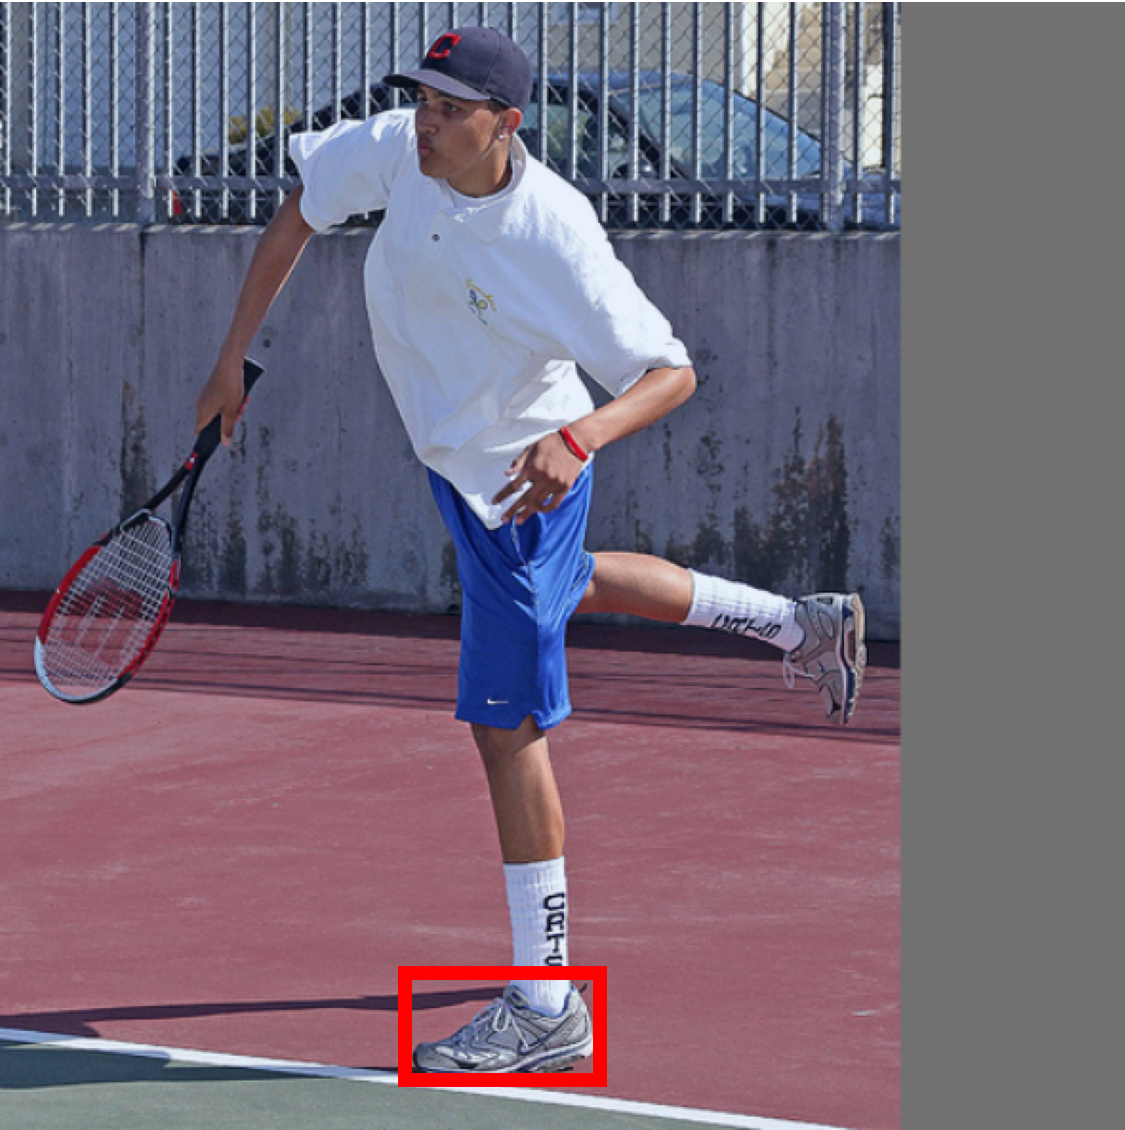
\includegraphics[width=0.9\linewidth]{figures/result/tennis/obj2}
	\end{minipage}}
	\subfigure[]{
		\begin{minipage}[t]{3.5cm}
			\centering
			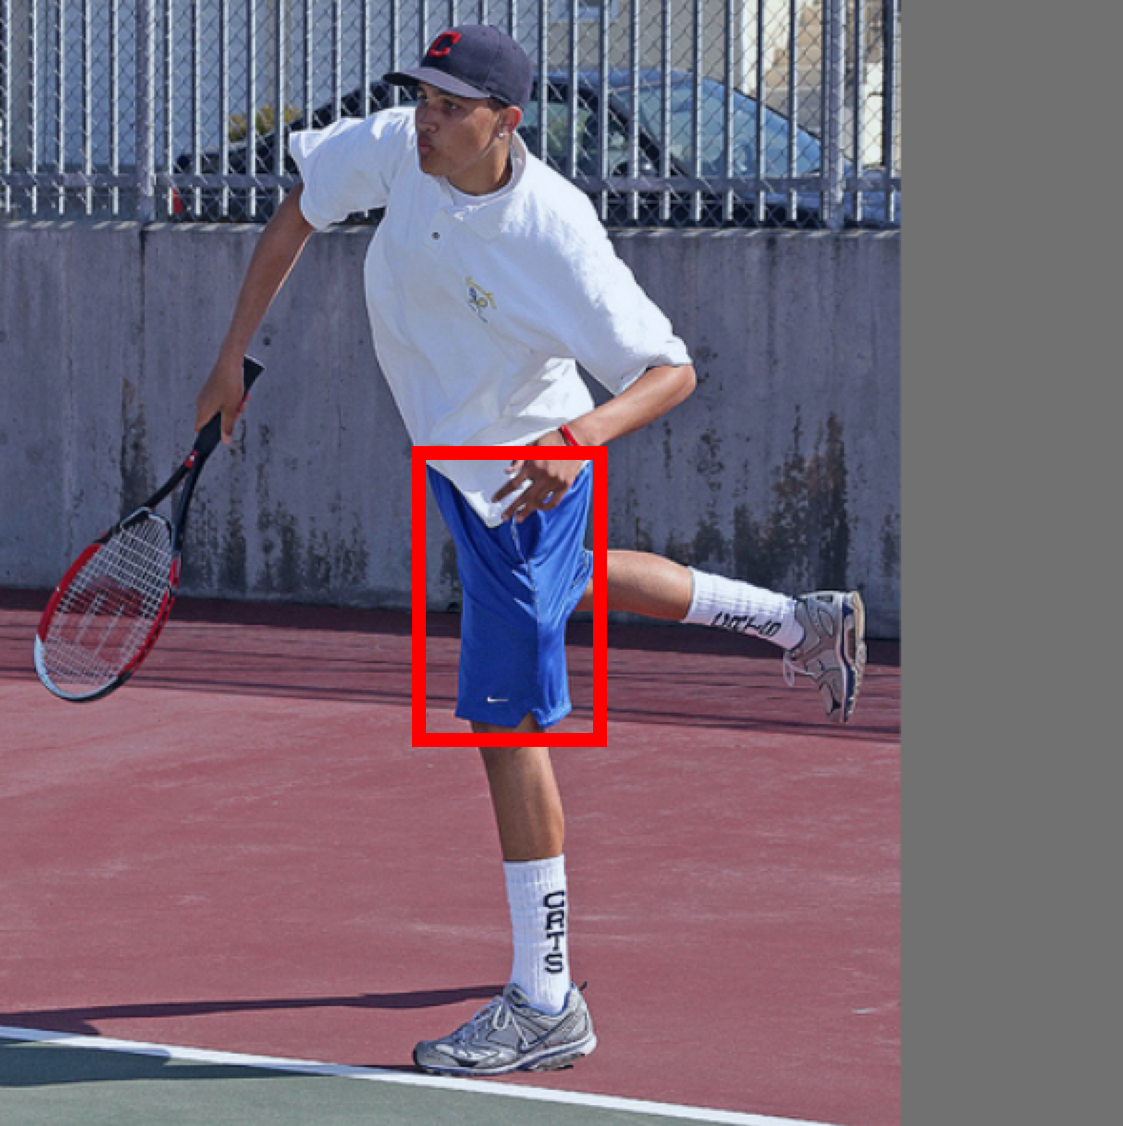
\includegraphics[width=0.9\linewidth]{figures/result/tennis/obj4}
	\end{minipage}}
	\subfigure[]{
		\begin{minipage}[t]{3.5cm}
			\centering
			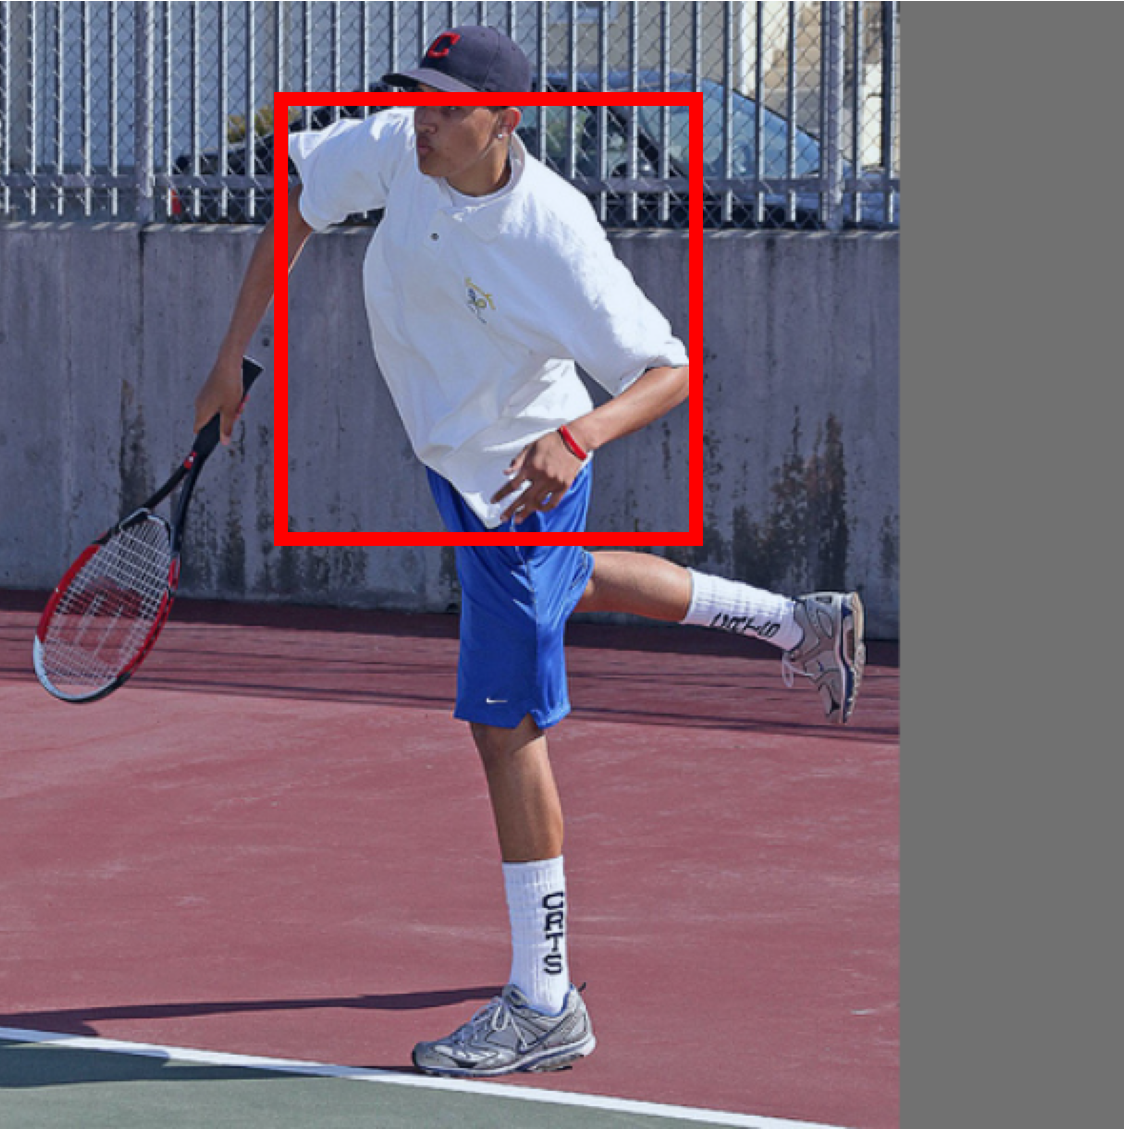
\includegraphics[width=0.9\linewidth]{figures/result/tennis/obj5}
	\end{minipage}}
	\subfigure[]{
		\begin{minipage}[t]{3.5cm}
			\centering
			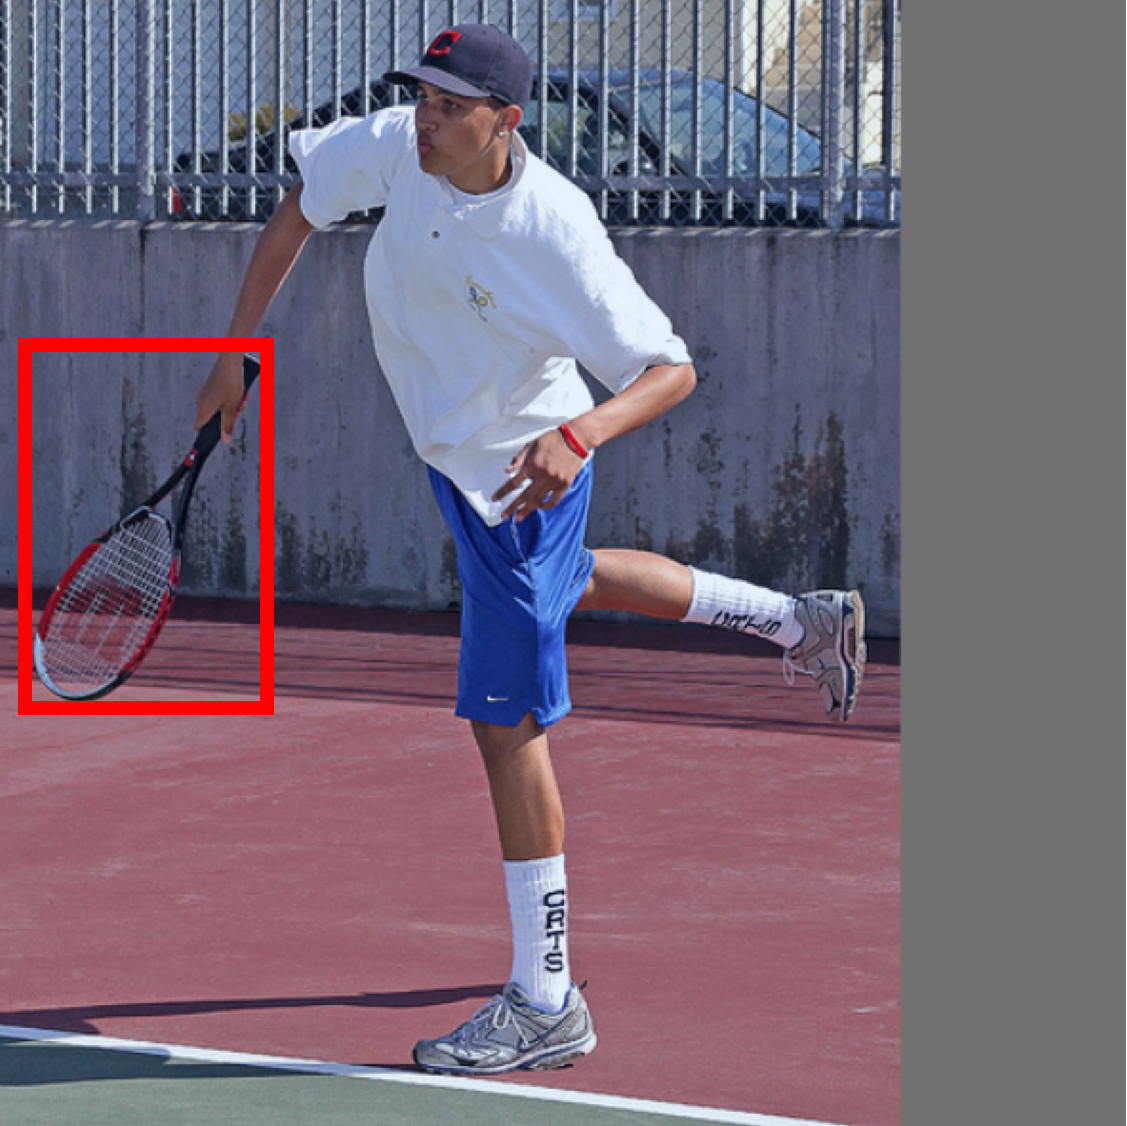
\includegraphics[width=0.9\linewidth]{figures/result/tennis/obj6}
	\end{minipage}}
	
	\subfigure[]{
		\begin{minipage}[t]{3.5cm}
			\centering
			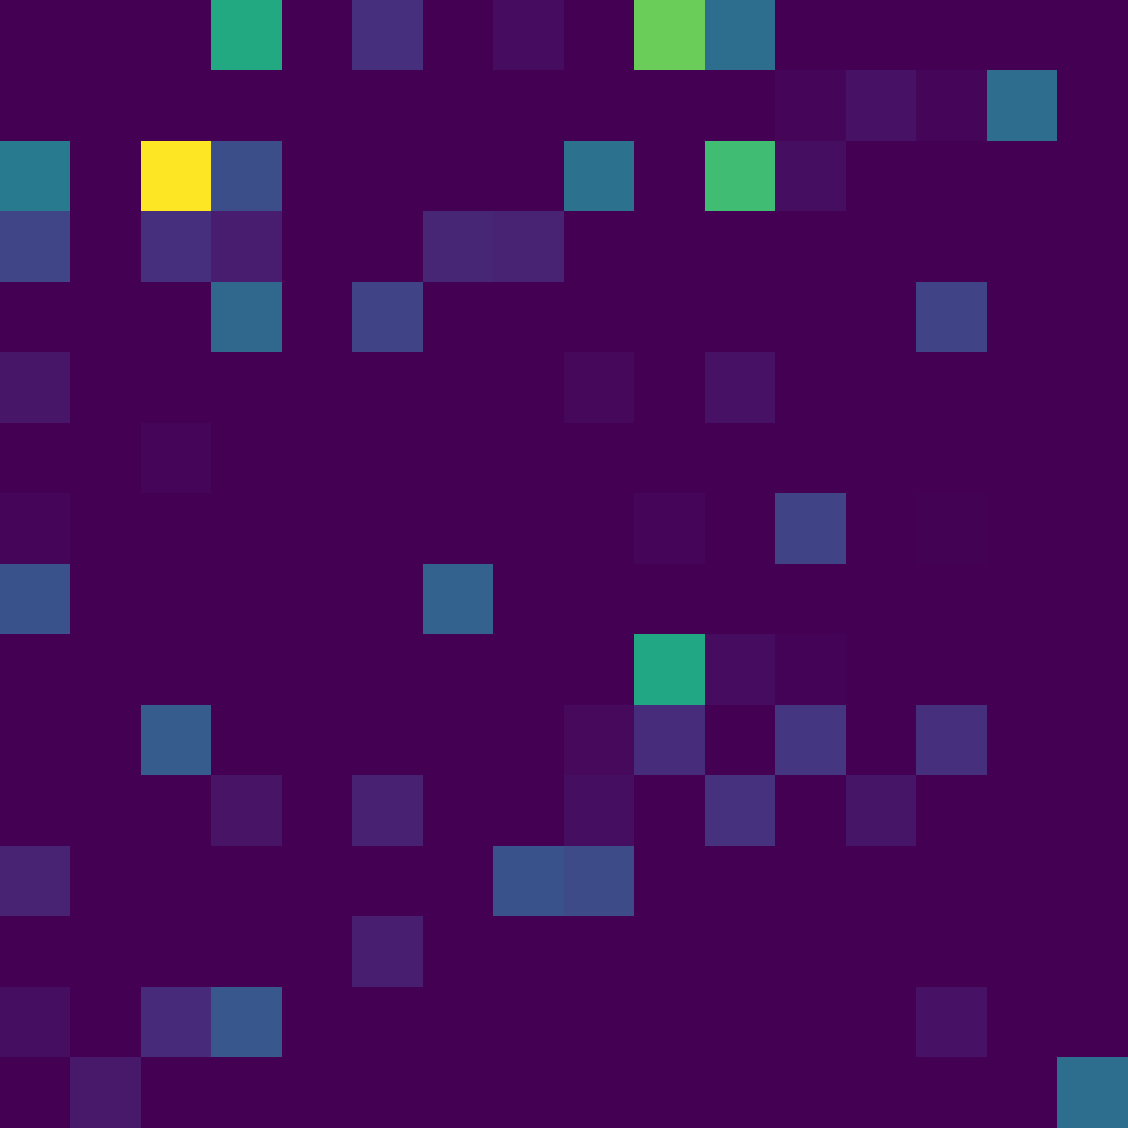
\includegraphics[width=0.9\linewidth]{figures/result/tennis/q0_2}
	\end{minipage}}
	\subfigure[]{
		\begin{minipage}[t]{3.5cm}
			\centering
			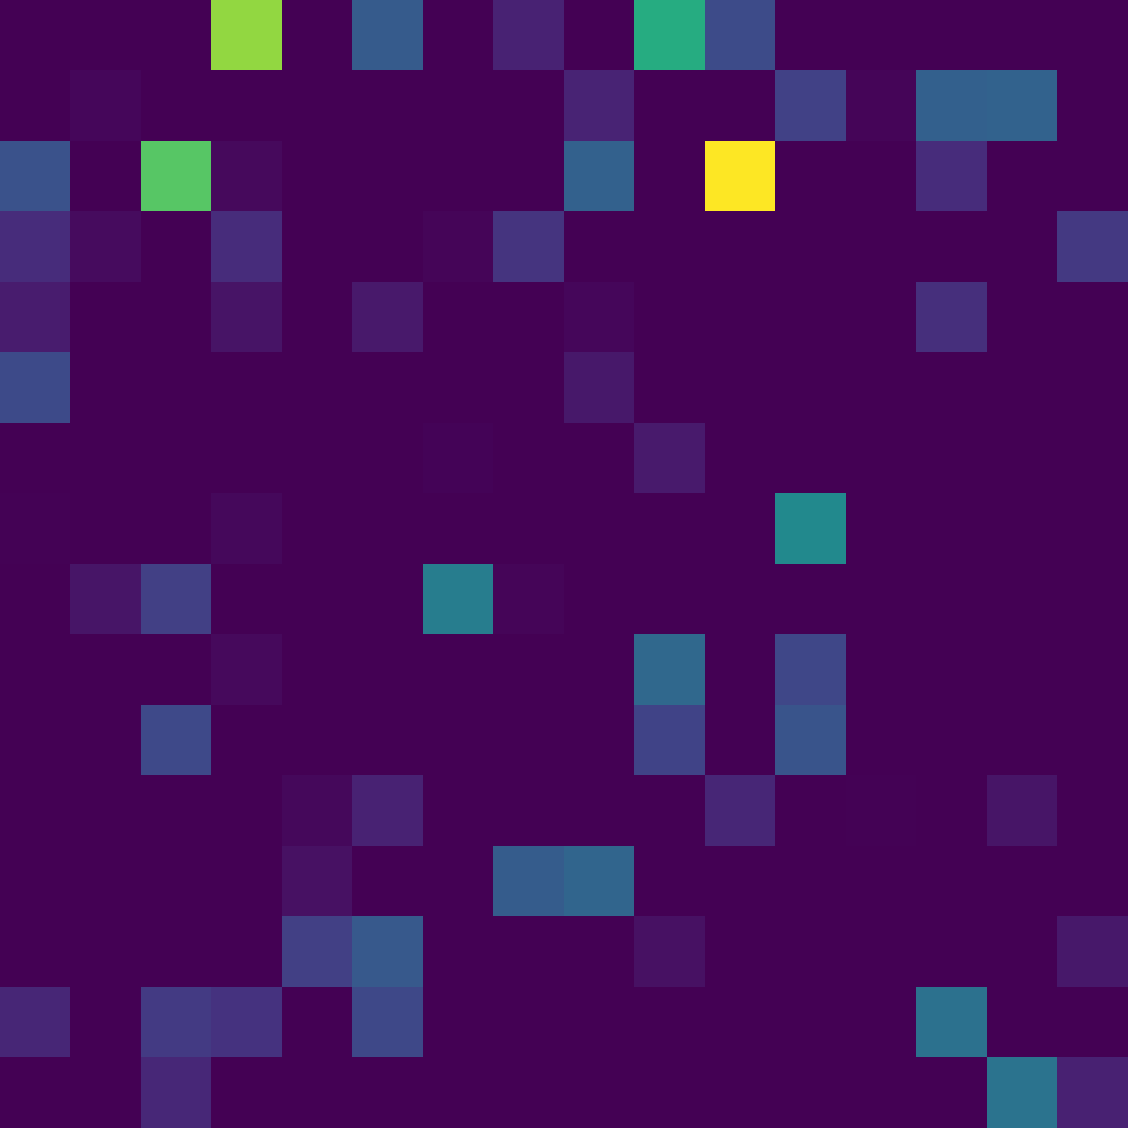
\includegraphics[width=0.9\linewidth]{figures/result/tennis/q0_4}
	\end{minipage}}
	\subfigure[]{
		\begin{minipage}[t]{3.5cm}
			\centering
			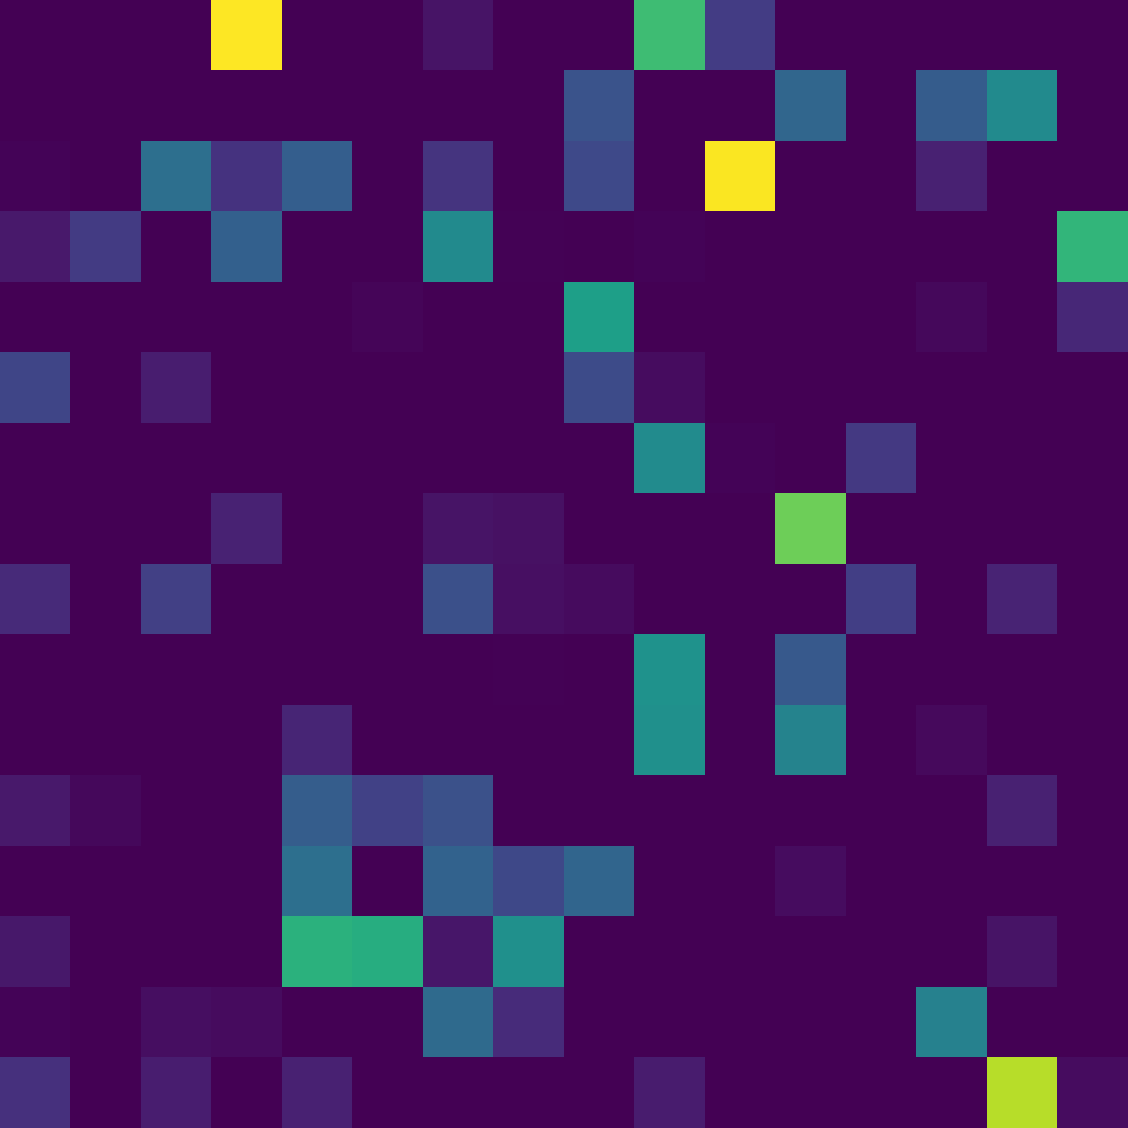
\includegraphics[width=0.9\linewidth]{figures/result/tennis/q0_5}
	\end{minipage}}
	\subfigure[]{
		\begin{minipage}[t]{3.5cm}
			\centering
			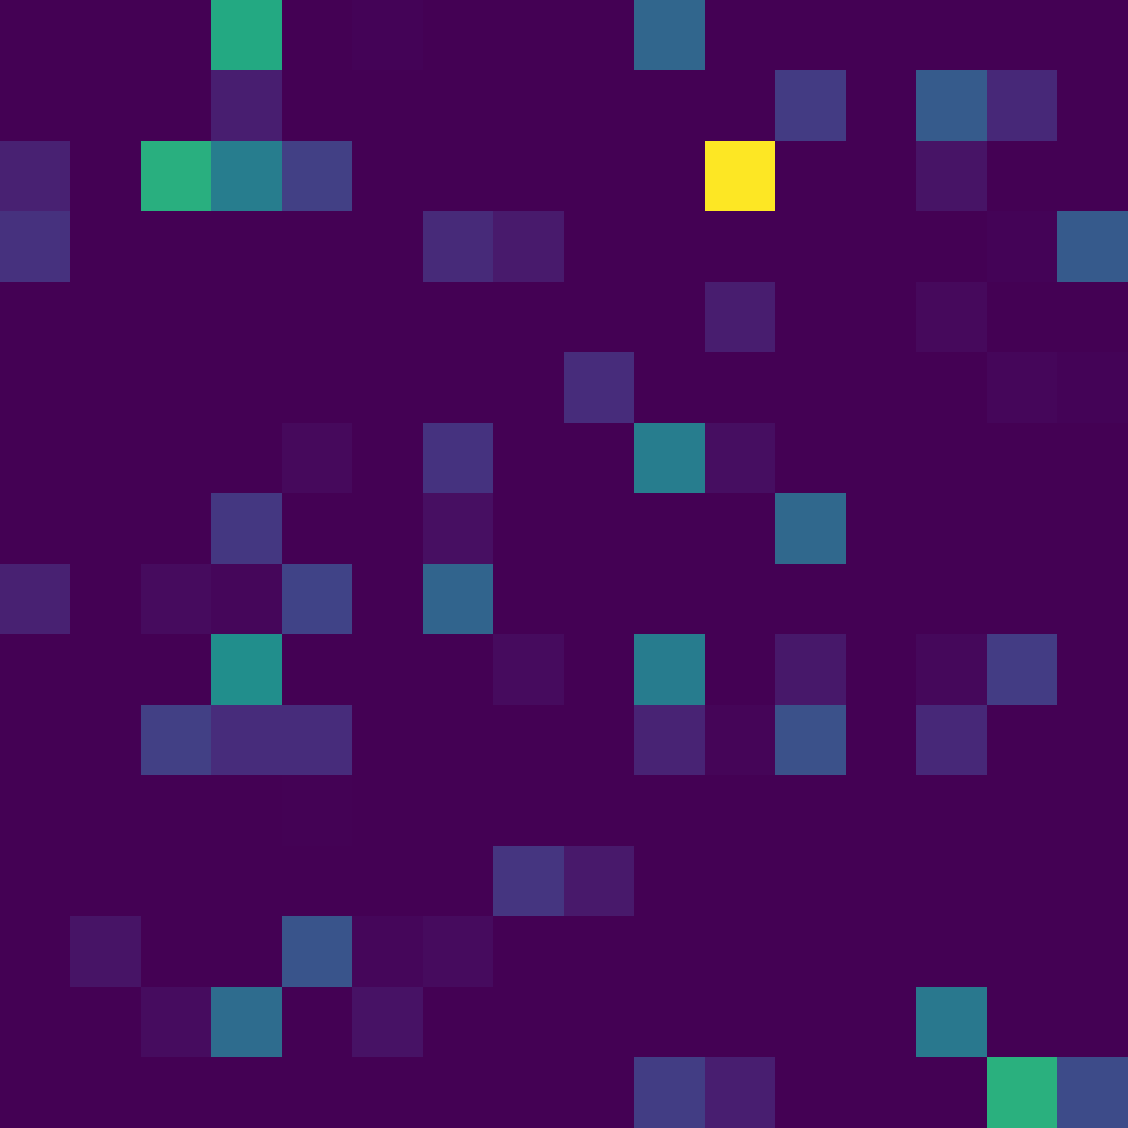
\includegraphics[width=0.9\linewidth]{figures/result/tennis/q0_6}
	\end{minipage}}

		\subfigure[]{
		\begin{minipage}[t]{3.5cm}
			\centering
			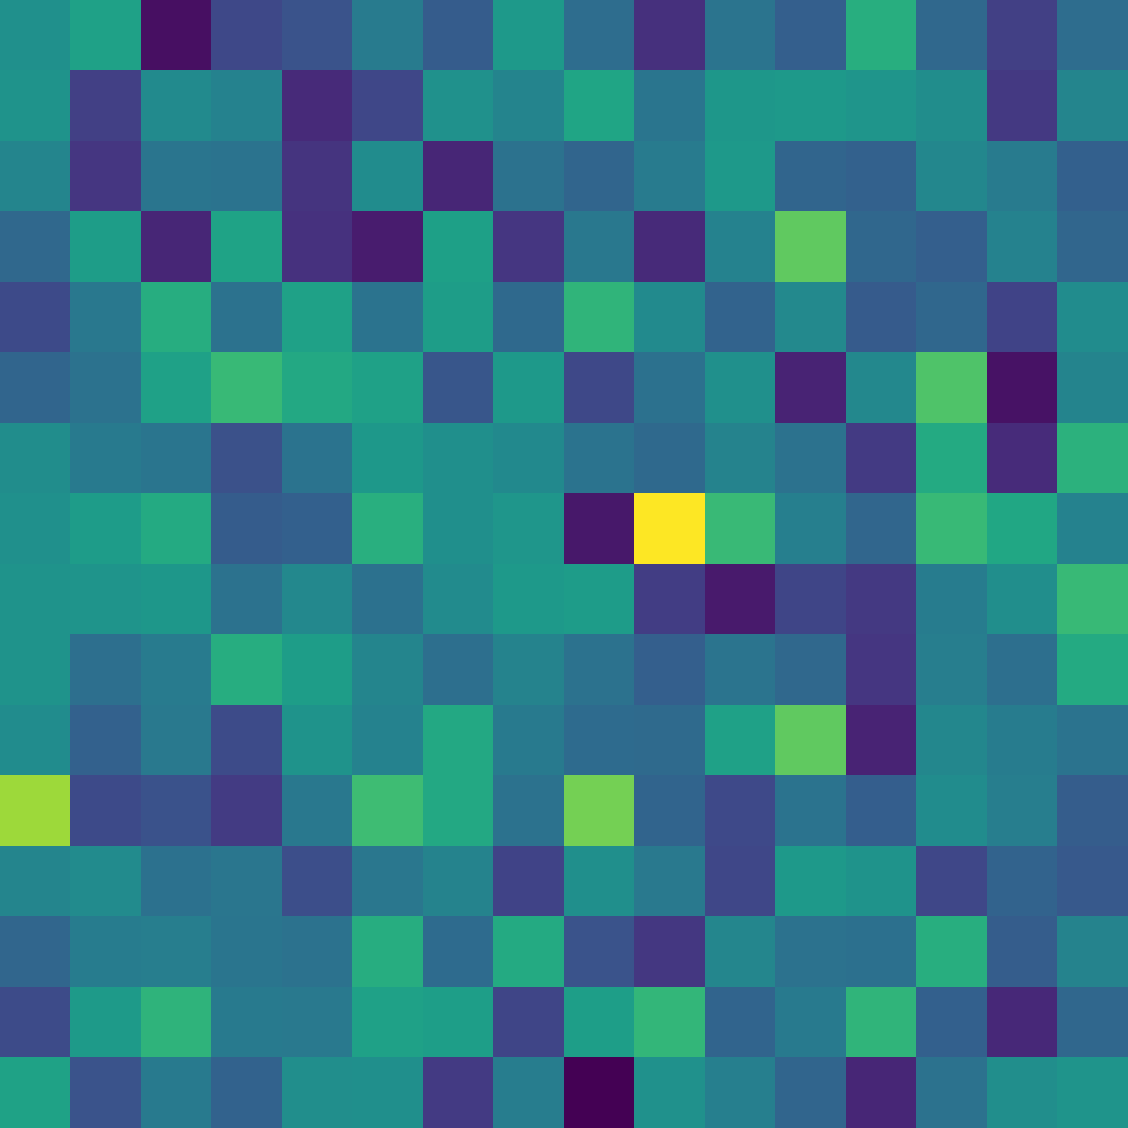
\includegraphics[width=0.9\linewidth]{figures/result/tennis/q3_2}
	\end{minipage}}
	\subfigure[]{
		\begin{minipage}[t]{3.5cm}
			\centering
			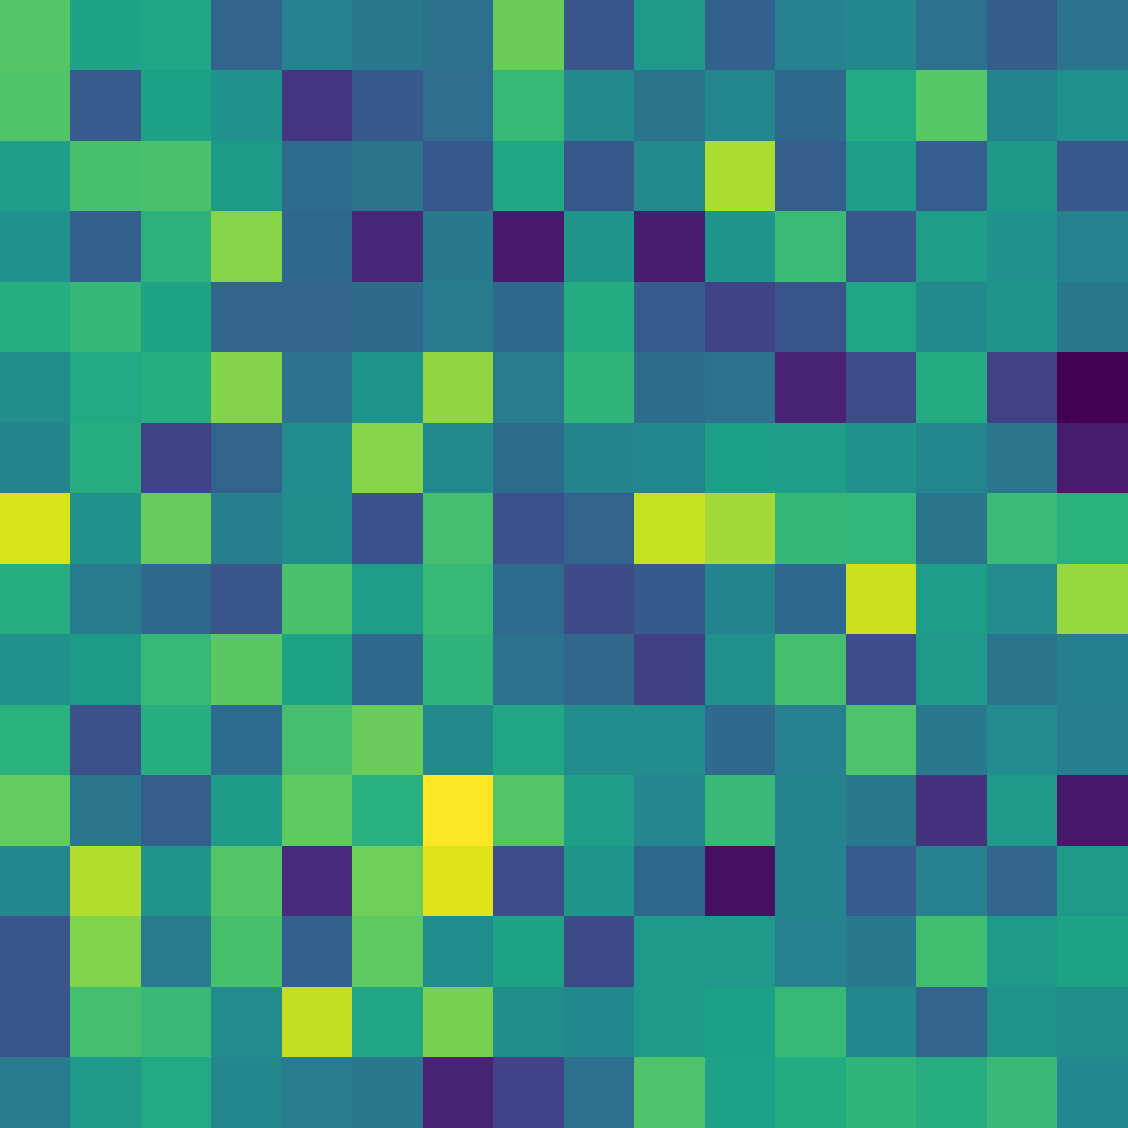
\includegraphics[width=0.9\linewidth]{figures/result/tennis/q3_4}
	\end{minipage}}
	\subfigure[]{
		\begin{minipage}[t]{3.5cm}
			\centering
			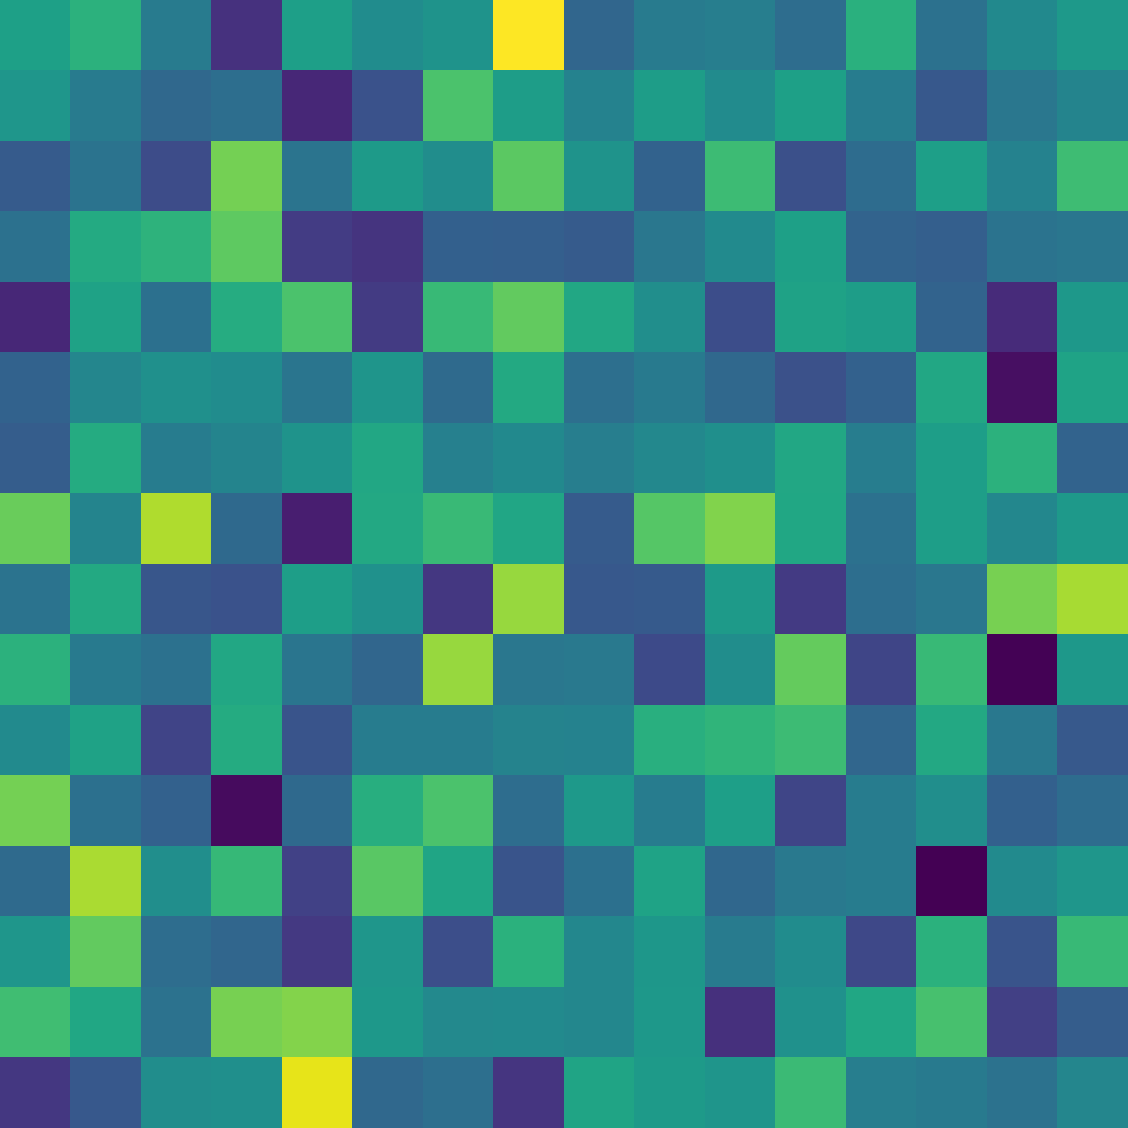
\includegraphics[width=0.9\linewidth]{figures/result/tennis/q3_5}
	\end{minipage}}
	\subfigure[]{
		\begin{minipage}[t]{3.5cm}
			\centering
			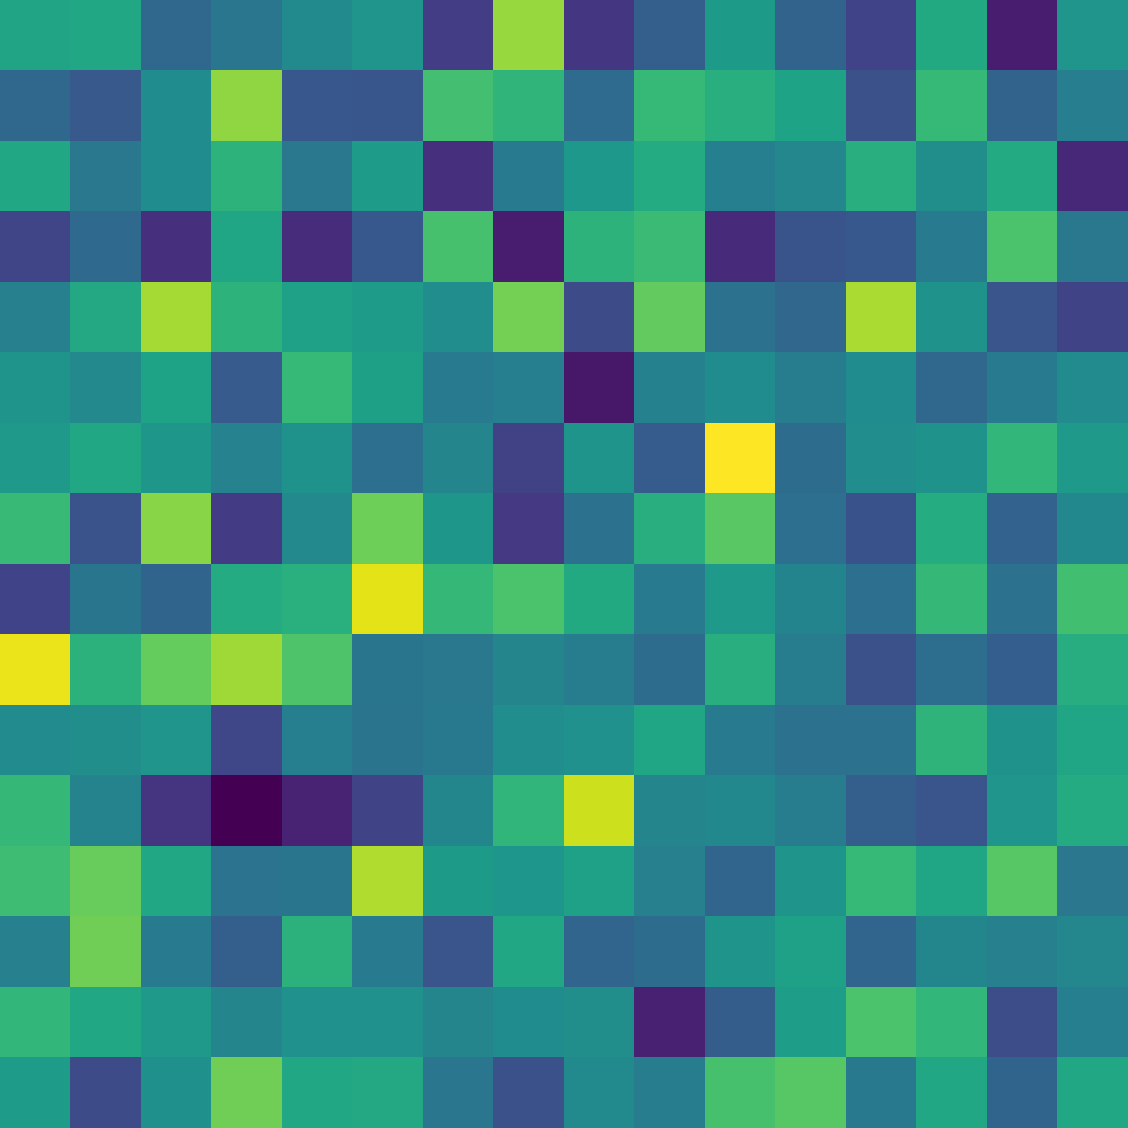
\includegraphics[width=0.9\linewidth]{figures/result/tennis/q3_6}
	\end{minipage}}

	\subfigure[]{
		\begin{minipage}[t]{3.5cm}
			\centering
			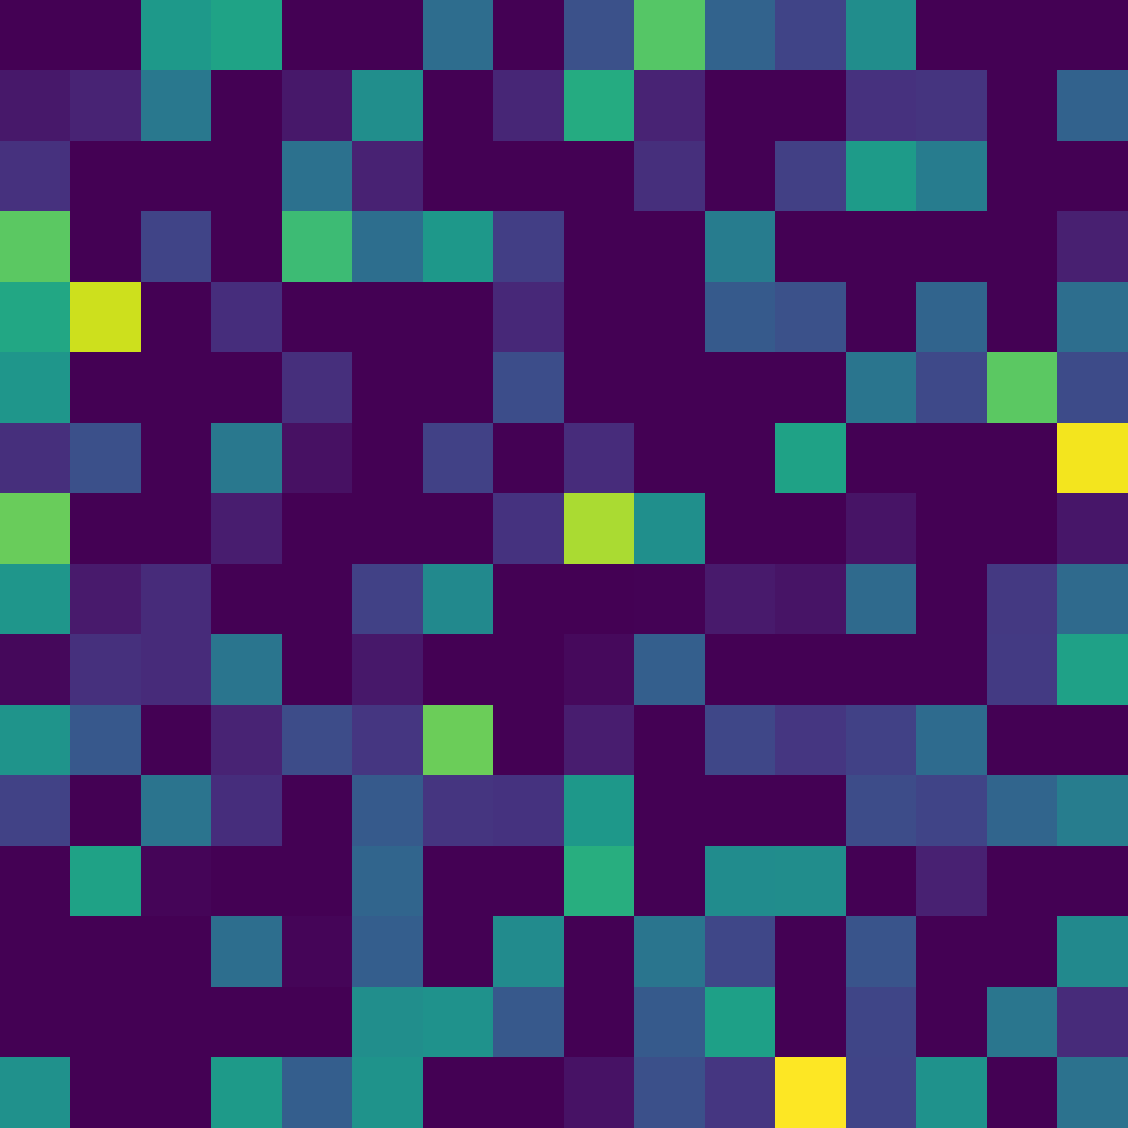
\includegraphics[width=0.9\linewidth]{figures/result/tennis/q2_2}
	\end{minipage}}
	\subfigure[]{
		\begin{minipage}[t]{3.5cm}
			\centering
			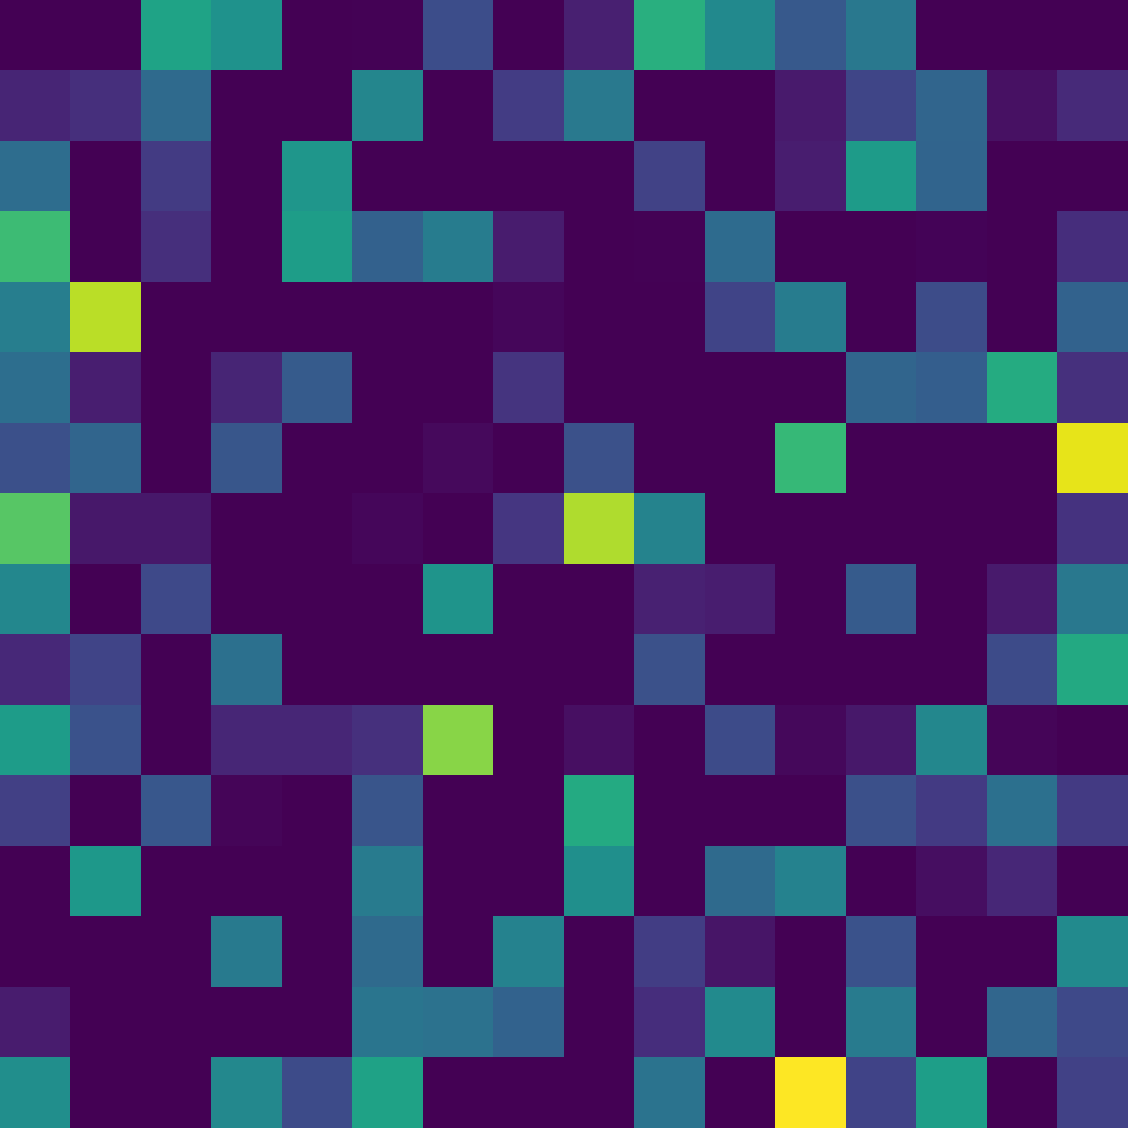
\includegraphics[width=0.9\linewidth]{figures/result/tennis/q2_4}
	\end{minipage}}
	\subfigure[]{
		\begin{minipage}[t]{3.5cm}
			\centering
			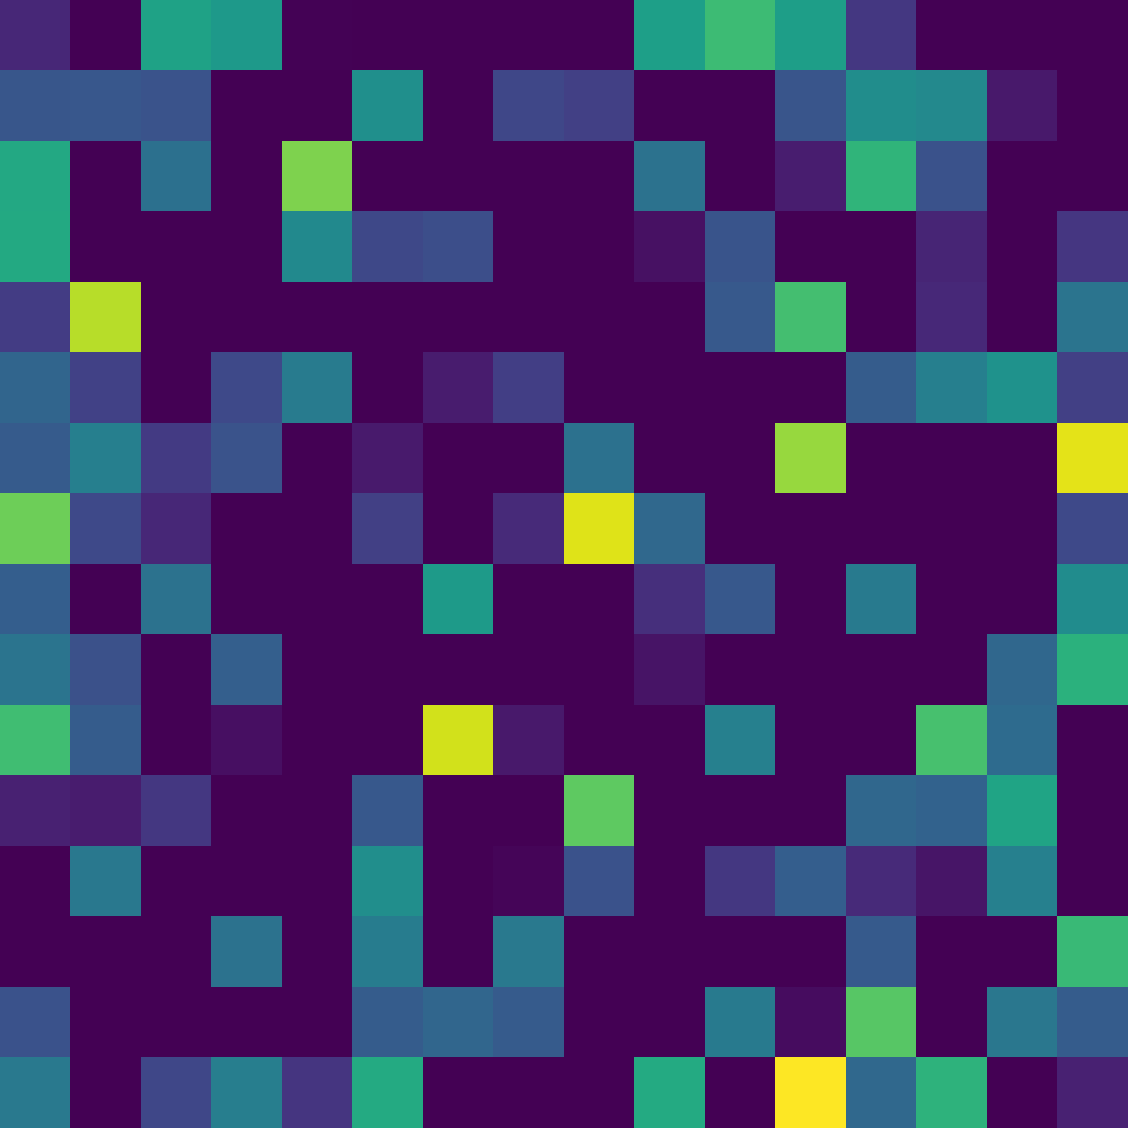
\includegraphics[width=0.9\linewidth]{figures/result/tennis/q2_5}
	\end{minipage}}
	\subfigure[]{
		\begin{minipage}[t]{3.5cm}
			\centering
			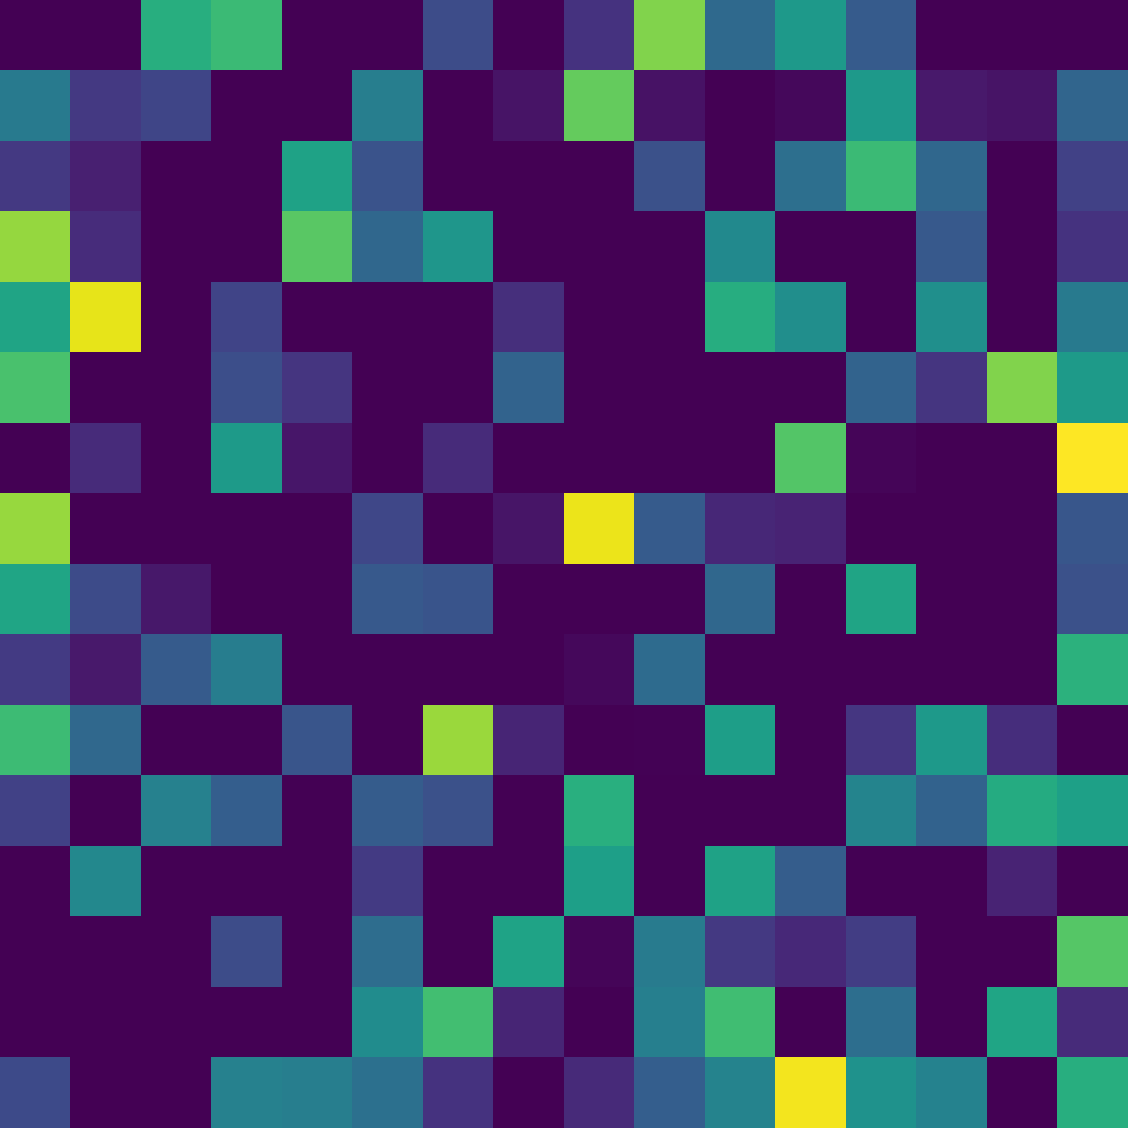
\includegraphics[width=0.9\linewidth]{figures/result/tennis/q2_6}
	\end{minipage}}
	
	\caption[An instance of Visualized results of the object query]{An instance of visualized results of the object query.from top to bottom, each row represents the position of the object, object query 1, object query 2 and object query 3.}
	\label{fig:tennis}
\end{figure}

\begin{figure}[h!]
	\centering
	\subfigure[]{
		\begin{minipage}[t]{3.5cm}
			\centering
			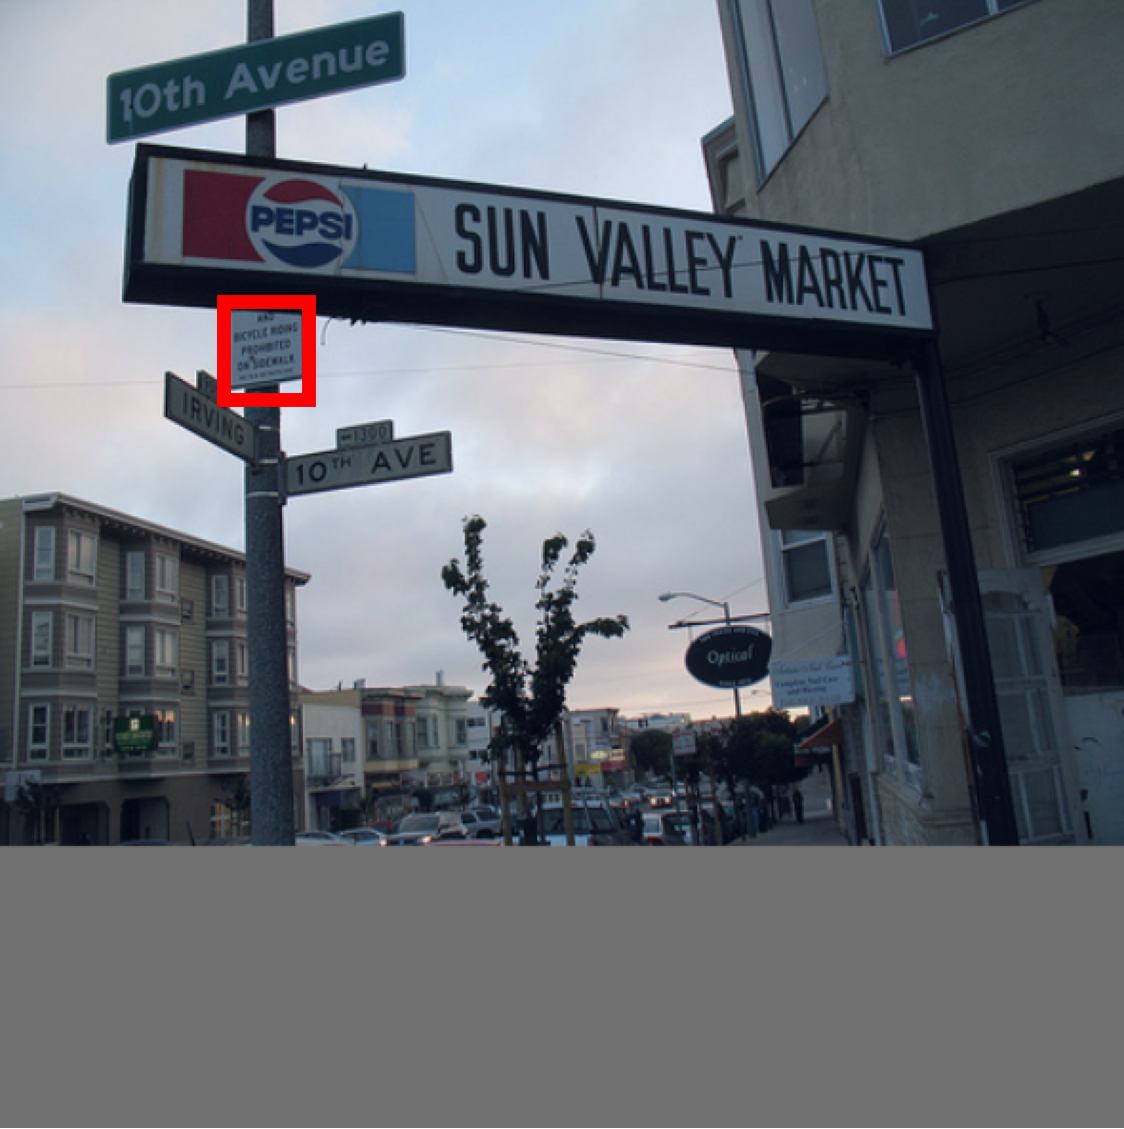
\includegraphics[width=0.9\linewidth]{figures/result/street/o1}
	\end{minipage}}
	\subfigure[]{
		\begin{minipage}[t]{3.5cm}
			\centering
			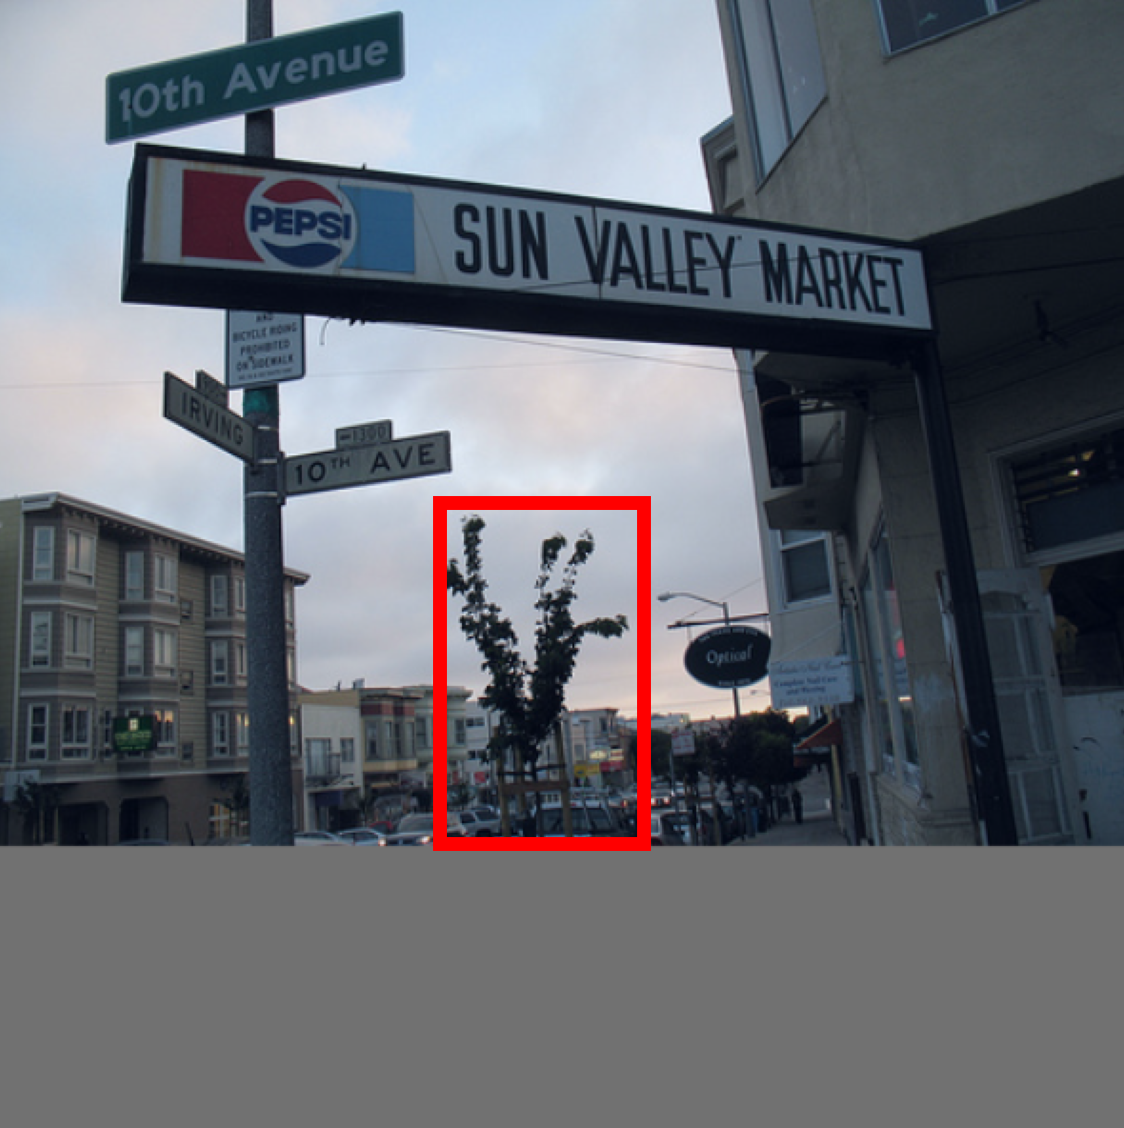
\includegraphics[width=0.9\linewidth]{figures/result/street/o2}
	\end{minipage}}
	\subfigure[]{
		\begin{minipage}[t]{3.5cm}
			\centering
			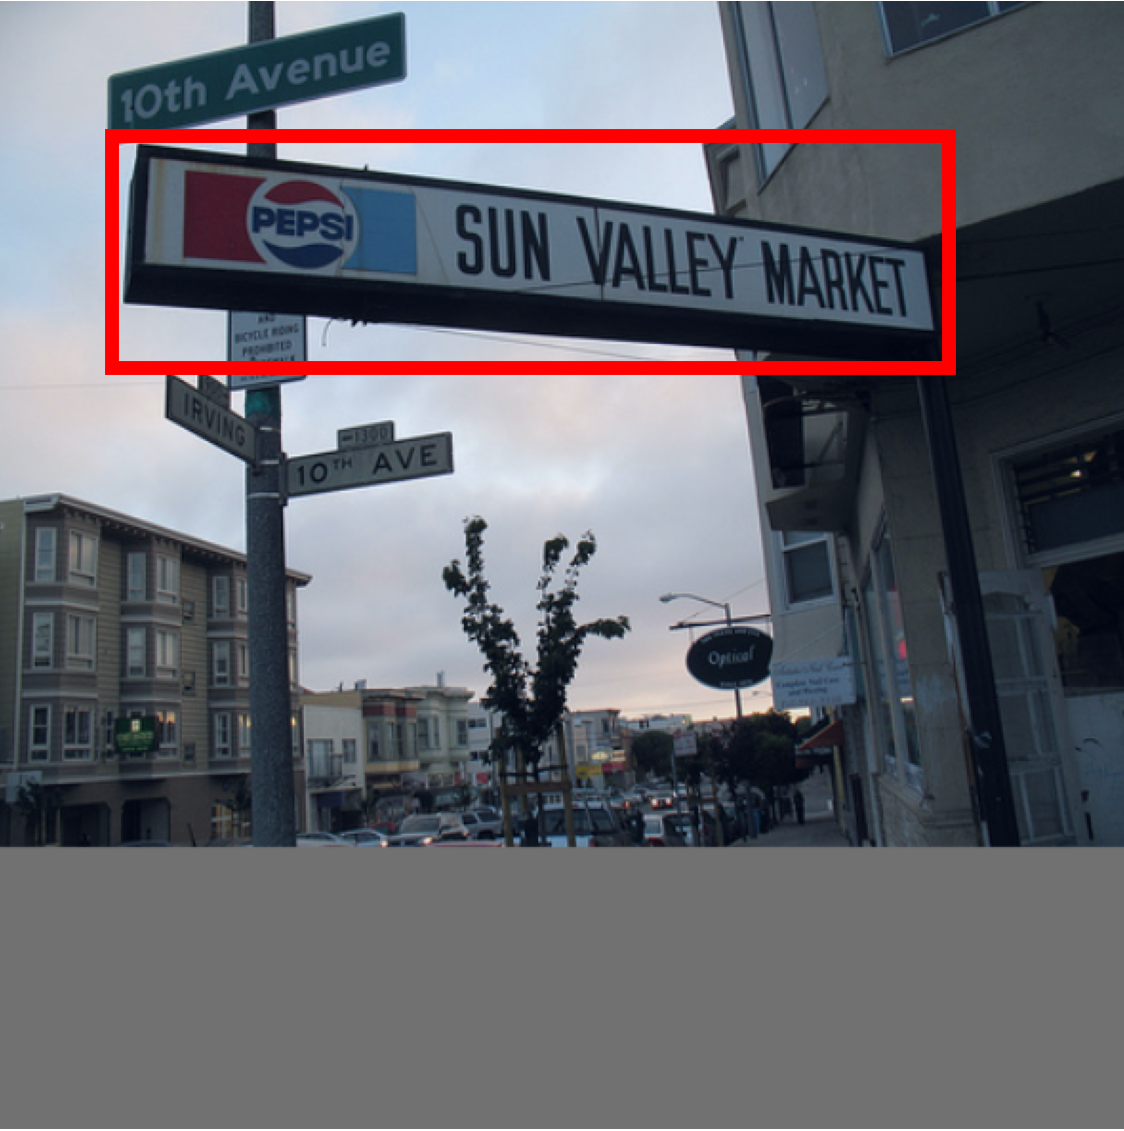
\includegraphics[width=0.9\linewidth]{figures/result/street/o3}
	\end{minipage}}
	\subfigure[]{
		\begin{minipage}[t]{3.5cm}
			\centering
			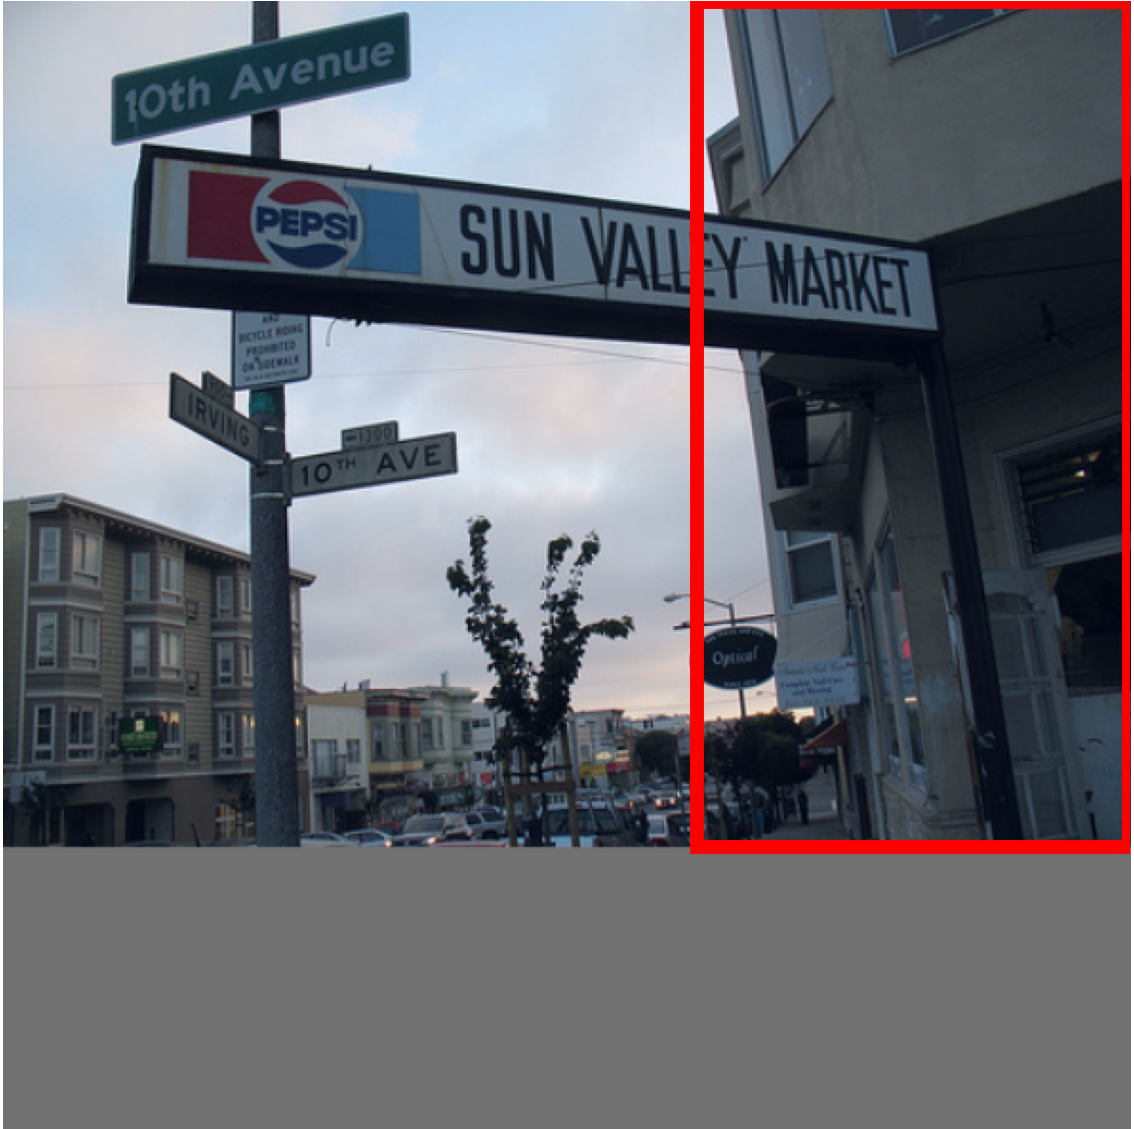
\includegraphics[width=0.9\linewidth]{figures/result/street/o4}
	\end{minipage}}
	
	\subfigure[]{
		\begin{minipage}[t]{3.5cm}
			\centering
			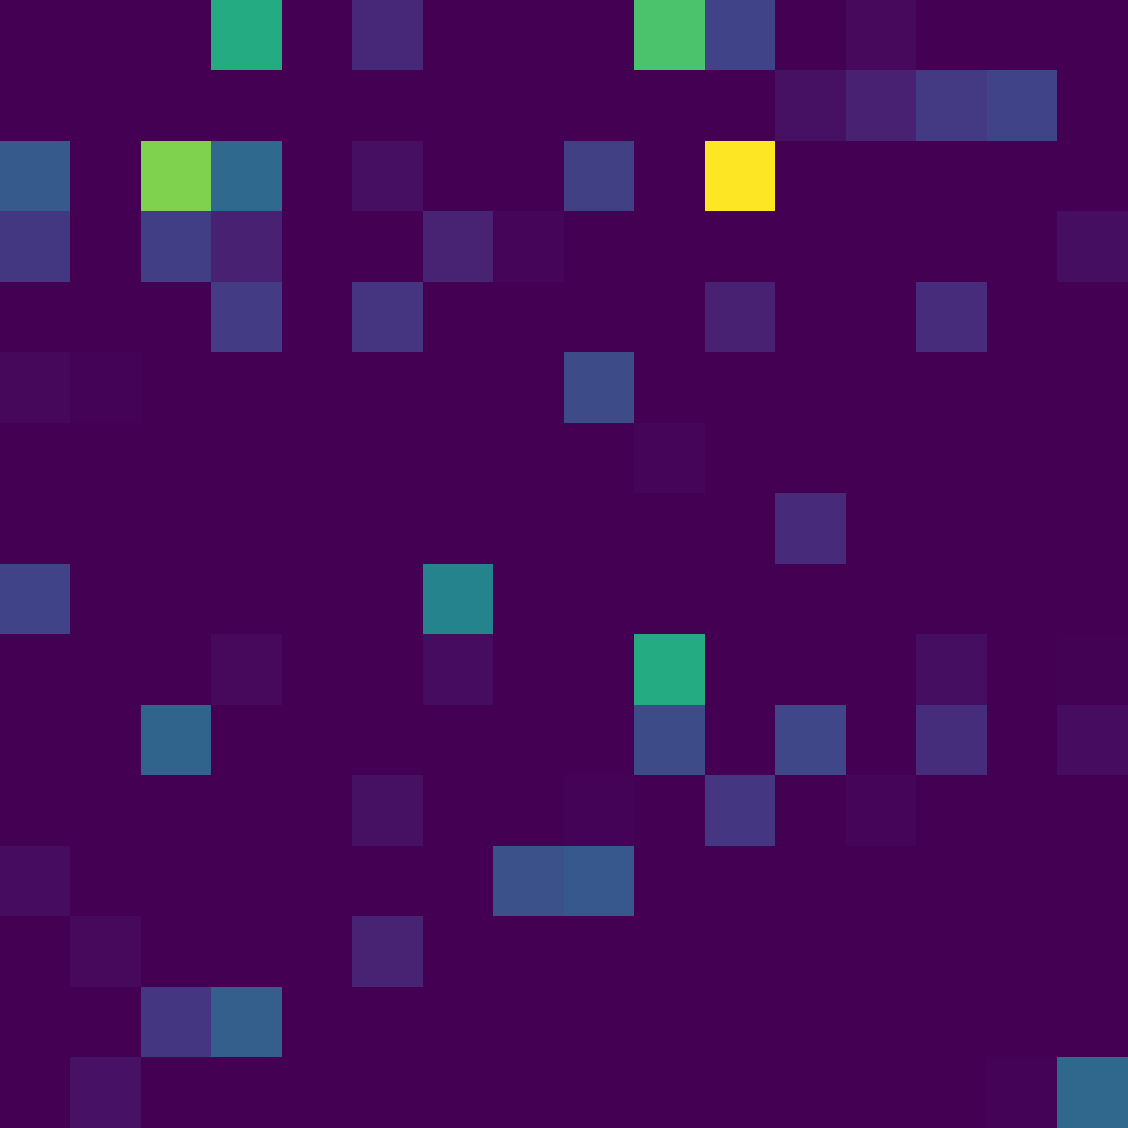
\includegraphics[width=0.9\linewidth]{figures/result/street/q0_1}
	\end{minipage}}
	\subfigure[]{
		\begin{minipage}[t]{3.5cm}
			\centering
			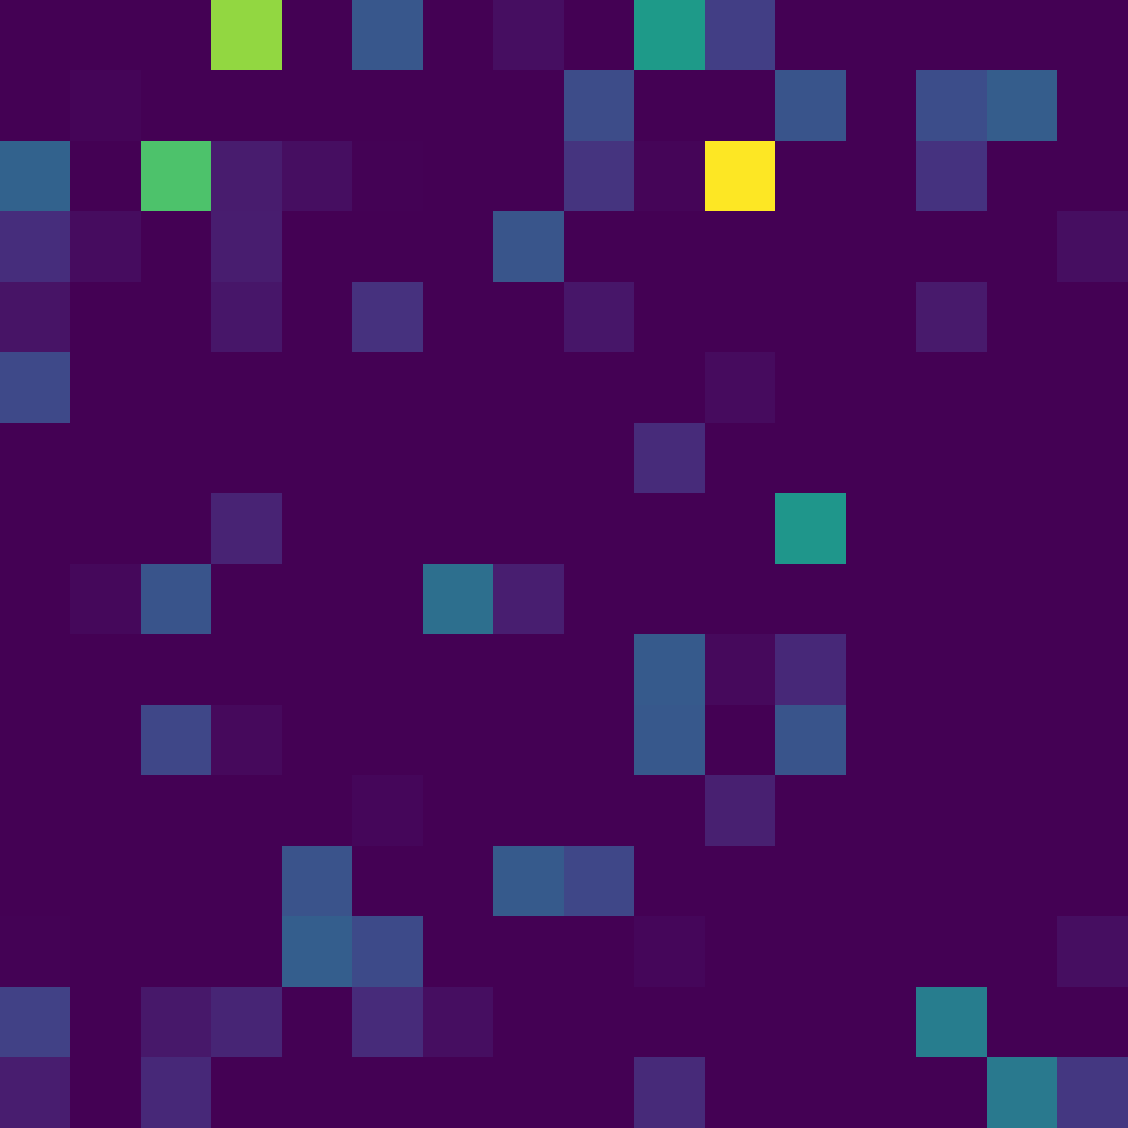
\includegraphics[width=0.9\linewidth]{figures/result/street/q0_2}
	\end{minipage}}
	\subfigure[]{
		\begin{minipage}[t]{3.5cm}
			\centering
			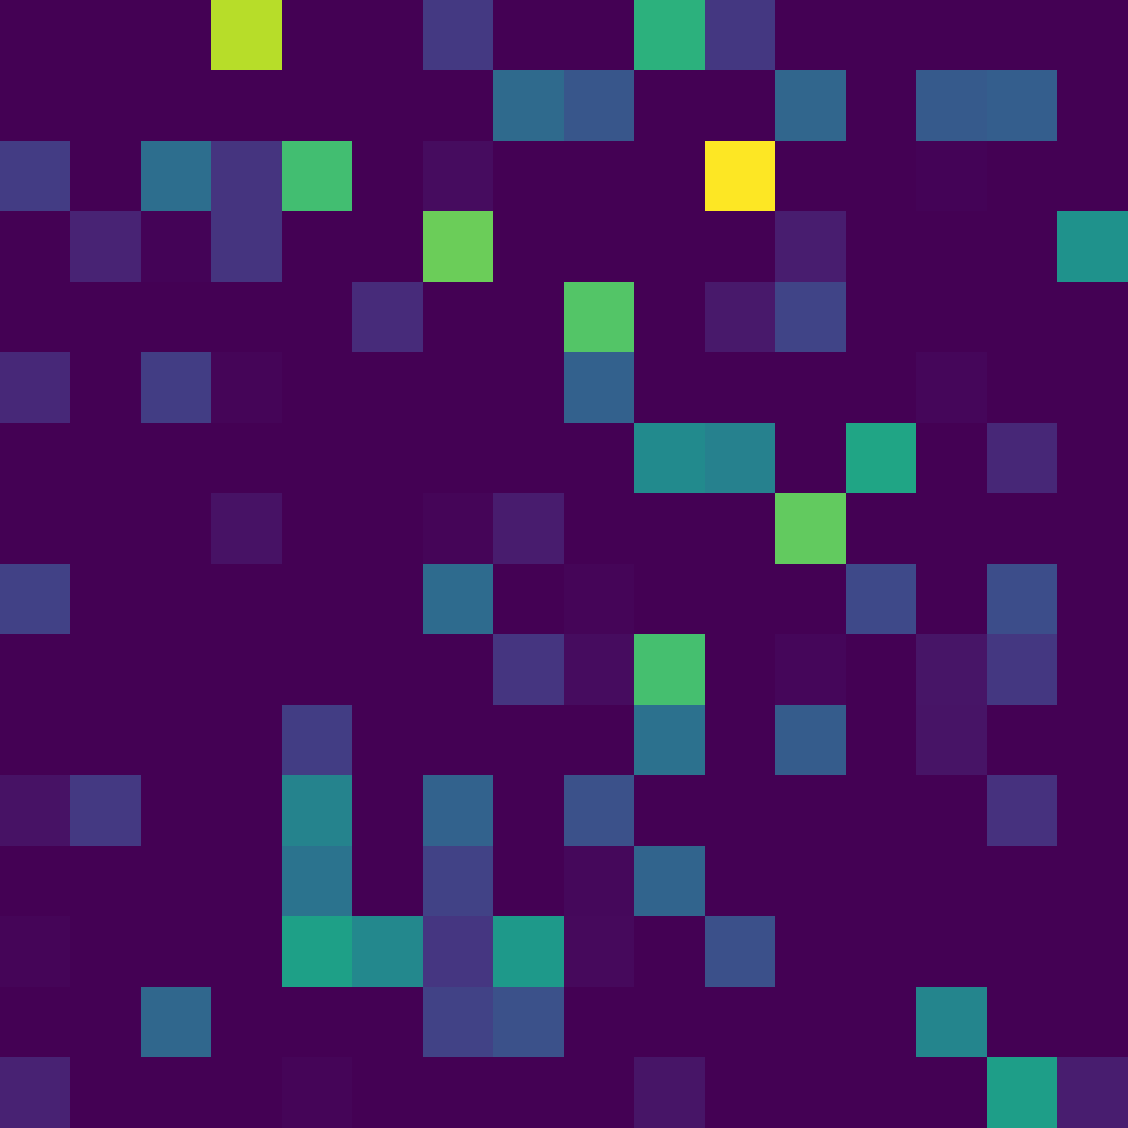
\includegraphics[width=0.9\linewidth]{figures/result/street/q0_3}
	\end{minipage}}
	\subfigure[]{
		\begin{minipage}[t]{3.5cm}
			\centering
			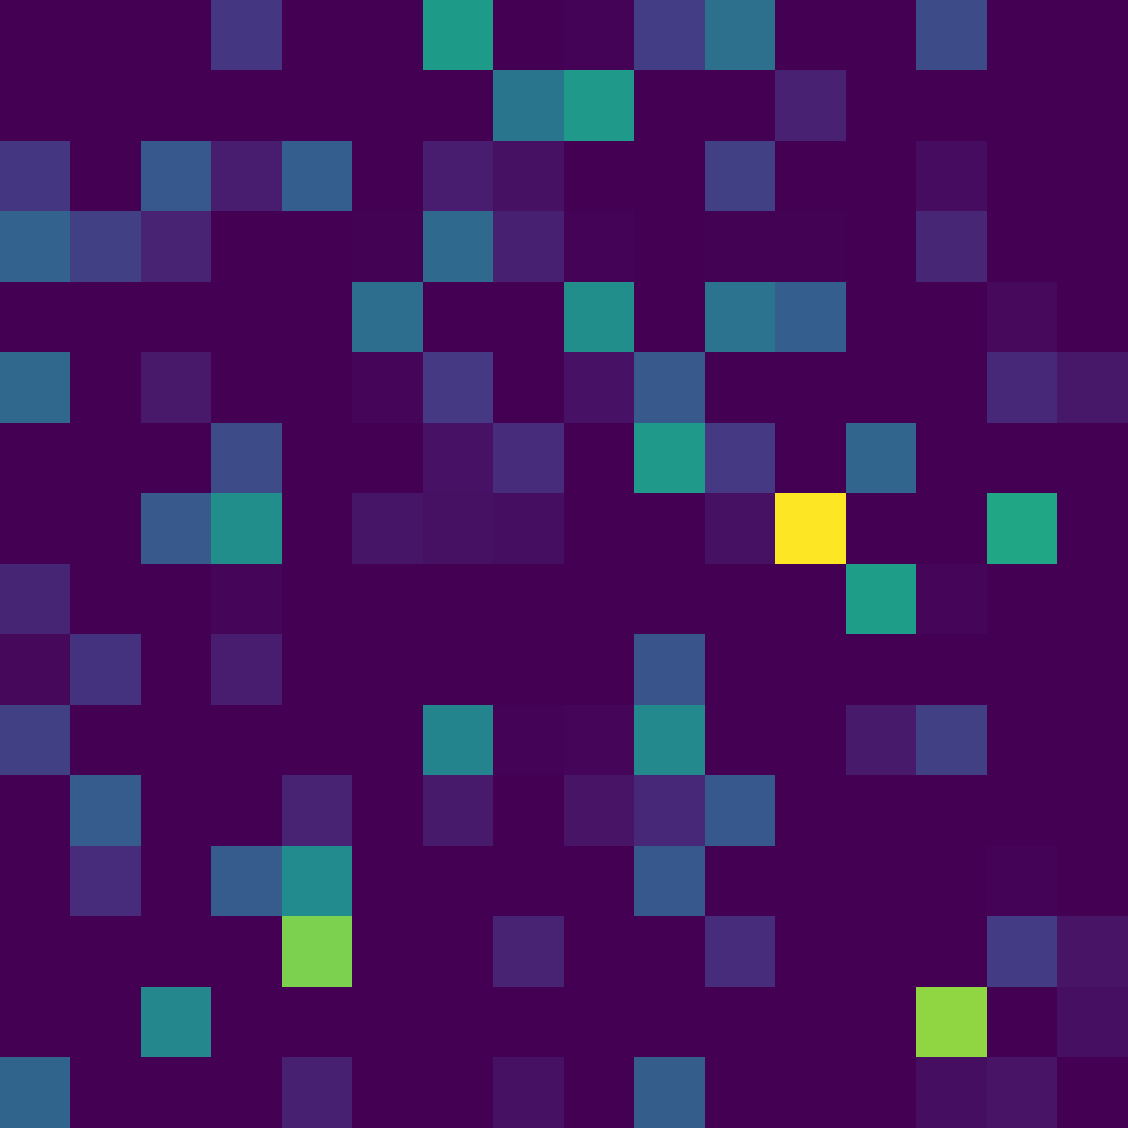
\includegraphics[width=0.9\linewidth]{figures/result/street/q0_4}
	\end{minipage}}
	
	\subfigure[]{
		\begin{minipage}[t]{3.5cm}
			\centering
			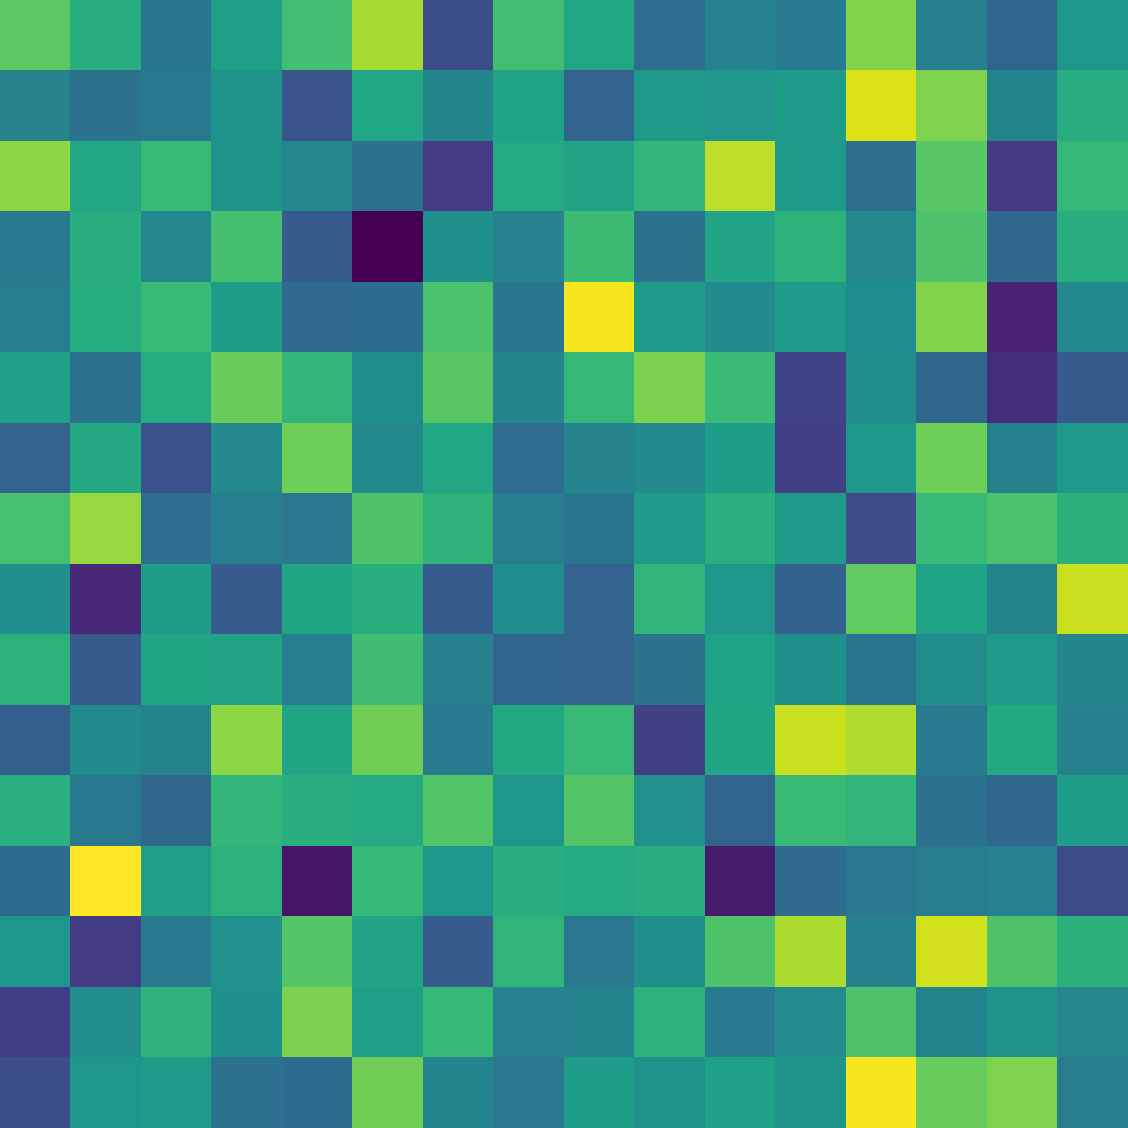
\includegraphics[width=0.9\linewidth]{figures/result/street/q3_1}
	\end{minipage}}
	\subfigure[]{
		\begin{minipage}[t]{3.5cm}
			\centering
			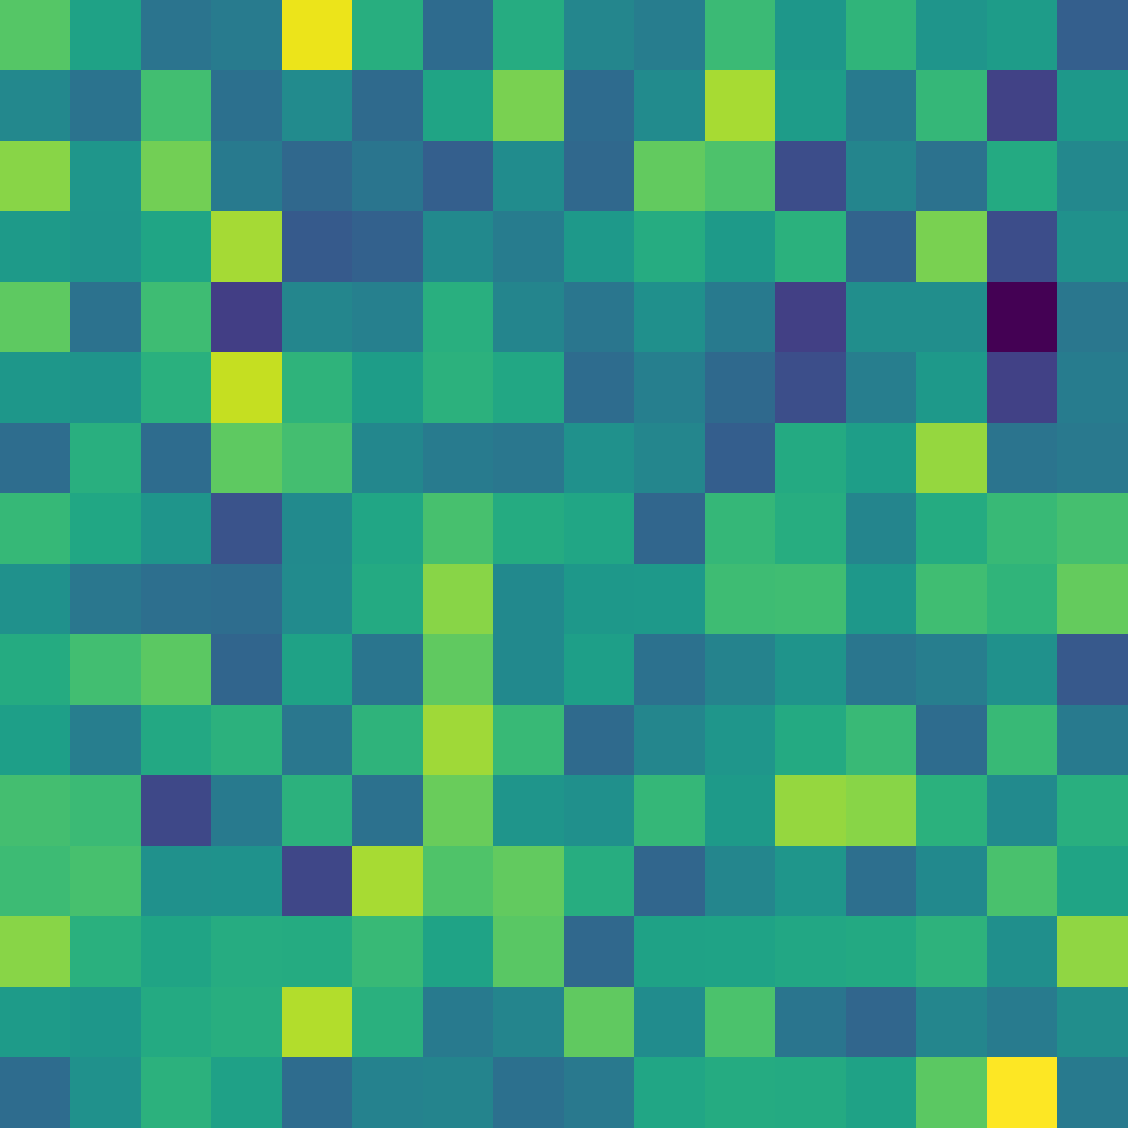
\includegraphics[width=0.9\linewidth]{figures/result/street/q3_2}
	\end{minipage}}
	\subfigure[]{
		\begin{minipage}[t]{3.5cm}
			\centering
			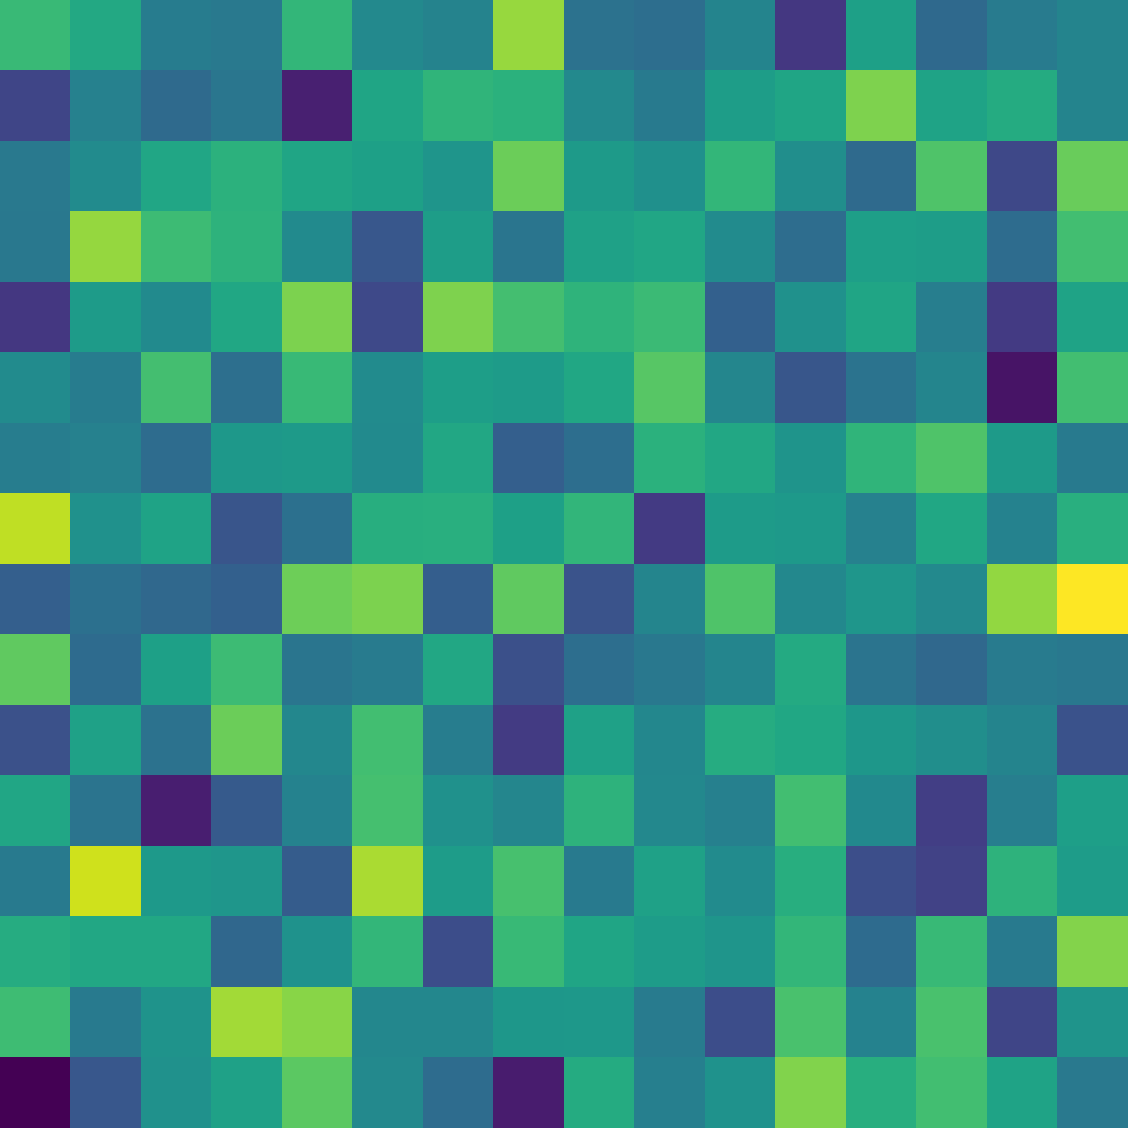
\includegraphics[width=0.9\linewidth]{figures/result/street/q3_3}
	\end{minipage}}
	\subfigure[]{
		\begin{minipage}[t]{3.5cm}
			\centering
			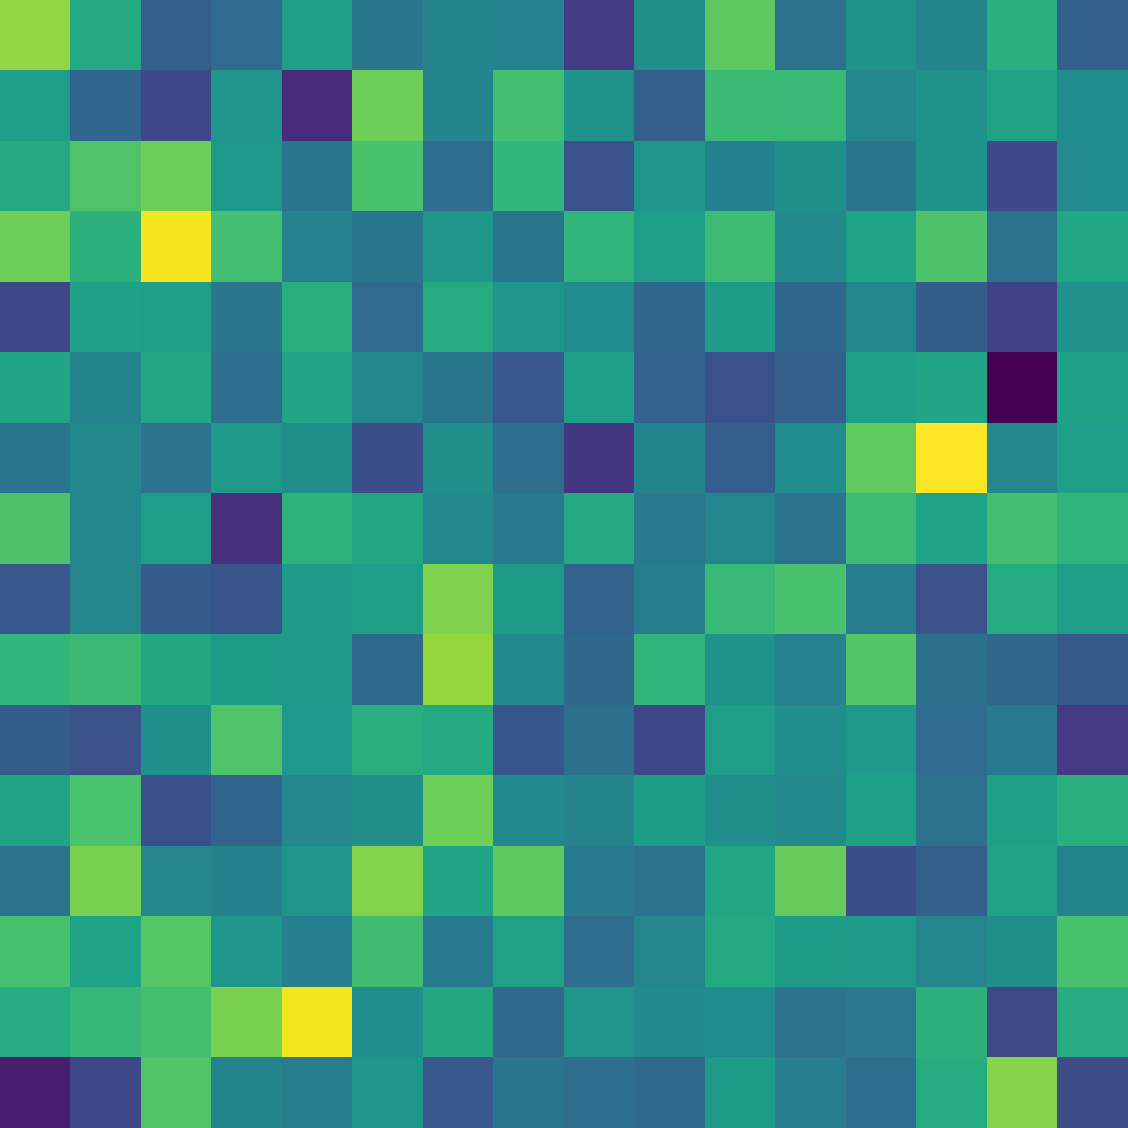
\includegraphics[width=0.9\linewidth]{figures/result/street/q3_4}
	\end{minipage}}

	\subfigure[]{
		\begin{minipage}[t]{3.5cm}
			\centering
			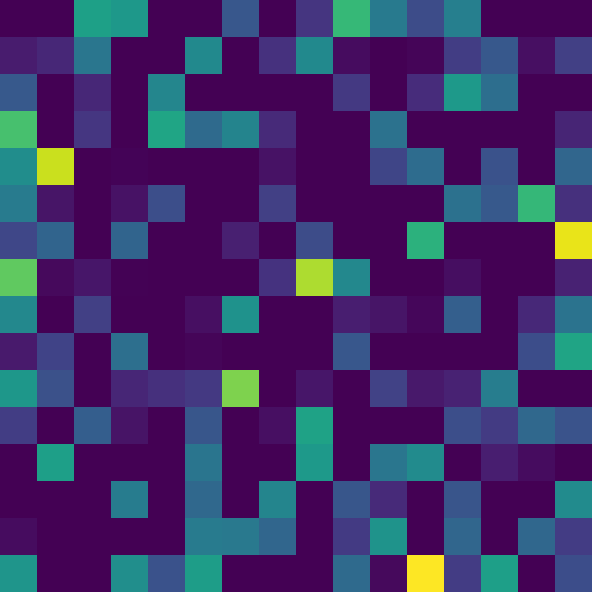
\includegraphics[width=0.9\linewidth]{figures/result/street/q2_1}
	\end{minipage}}
	\subfigure[]{
		\begin{minipage}[t]{3.5cm}
			\centering
			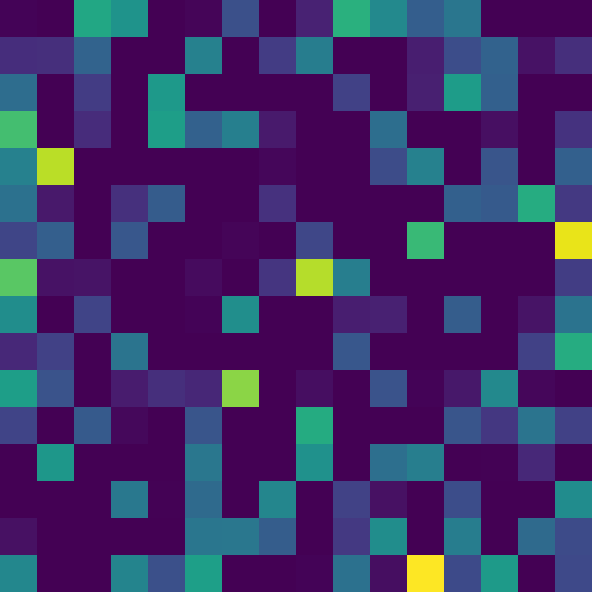
\includegraphics[width=0.9\linewidth]{figures/result/street/q2_2}
	\end{minipage}}
	\subfigure[]{
		\begin{minipage}[t]{3.5cm}
			\centering
			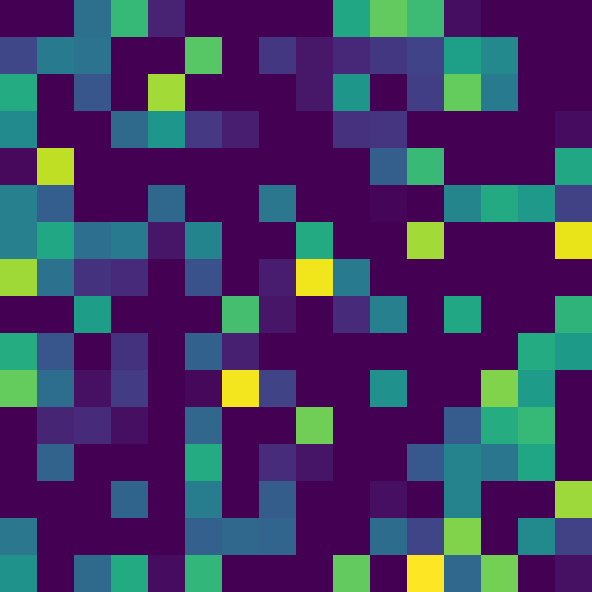
\includegraphics[width=0.9\linewidth]{figures/result/street/q2_3}
	\end{minipage}}
	\subfigure[]{
		\begin{minipage}[t]{3.5cm}
			\centering
			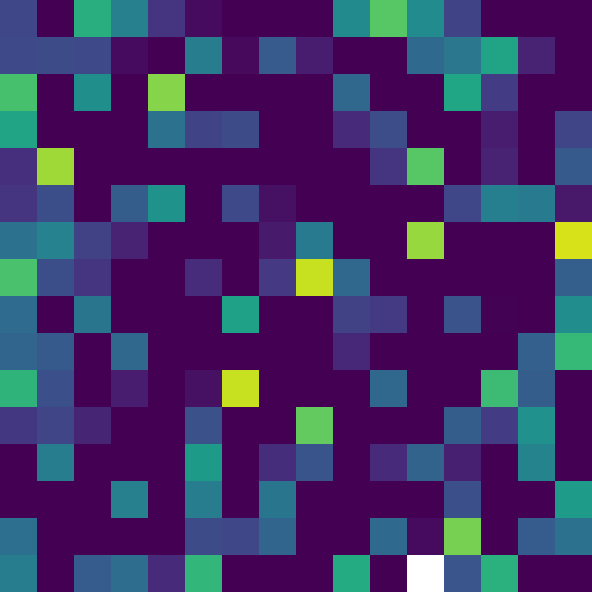
\includegraphics[width=0.9\linewidth]{figures/result/street/q2_4}
	\end{minipage}}

	
	\caption[An instance of Visualized results of the object query]{An instance of visualized results of the object query.from top to bottom, each row represents the position of the object, object query 1, object query 2 and object query 3.}
	\label{fig:street}
\end{figure}

\subsubsection{Result of our object query}
Next, we use our object query as the input of the object decoder to test the performance of these three queries in the task PredCLS, and we use recall@50 as the criterion.


\subsection{Experiment on Attention  Loss Function}

\begin{figure}[tbph!]
	\centering
	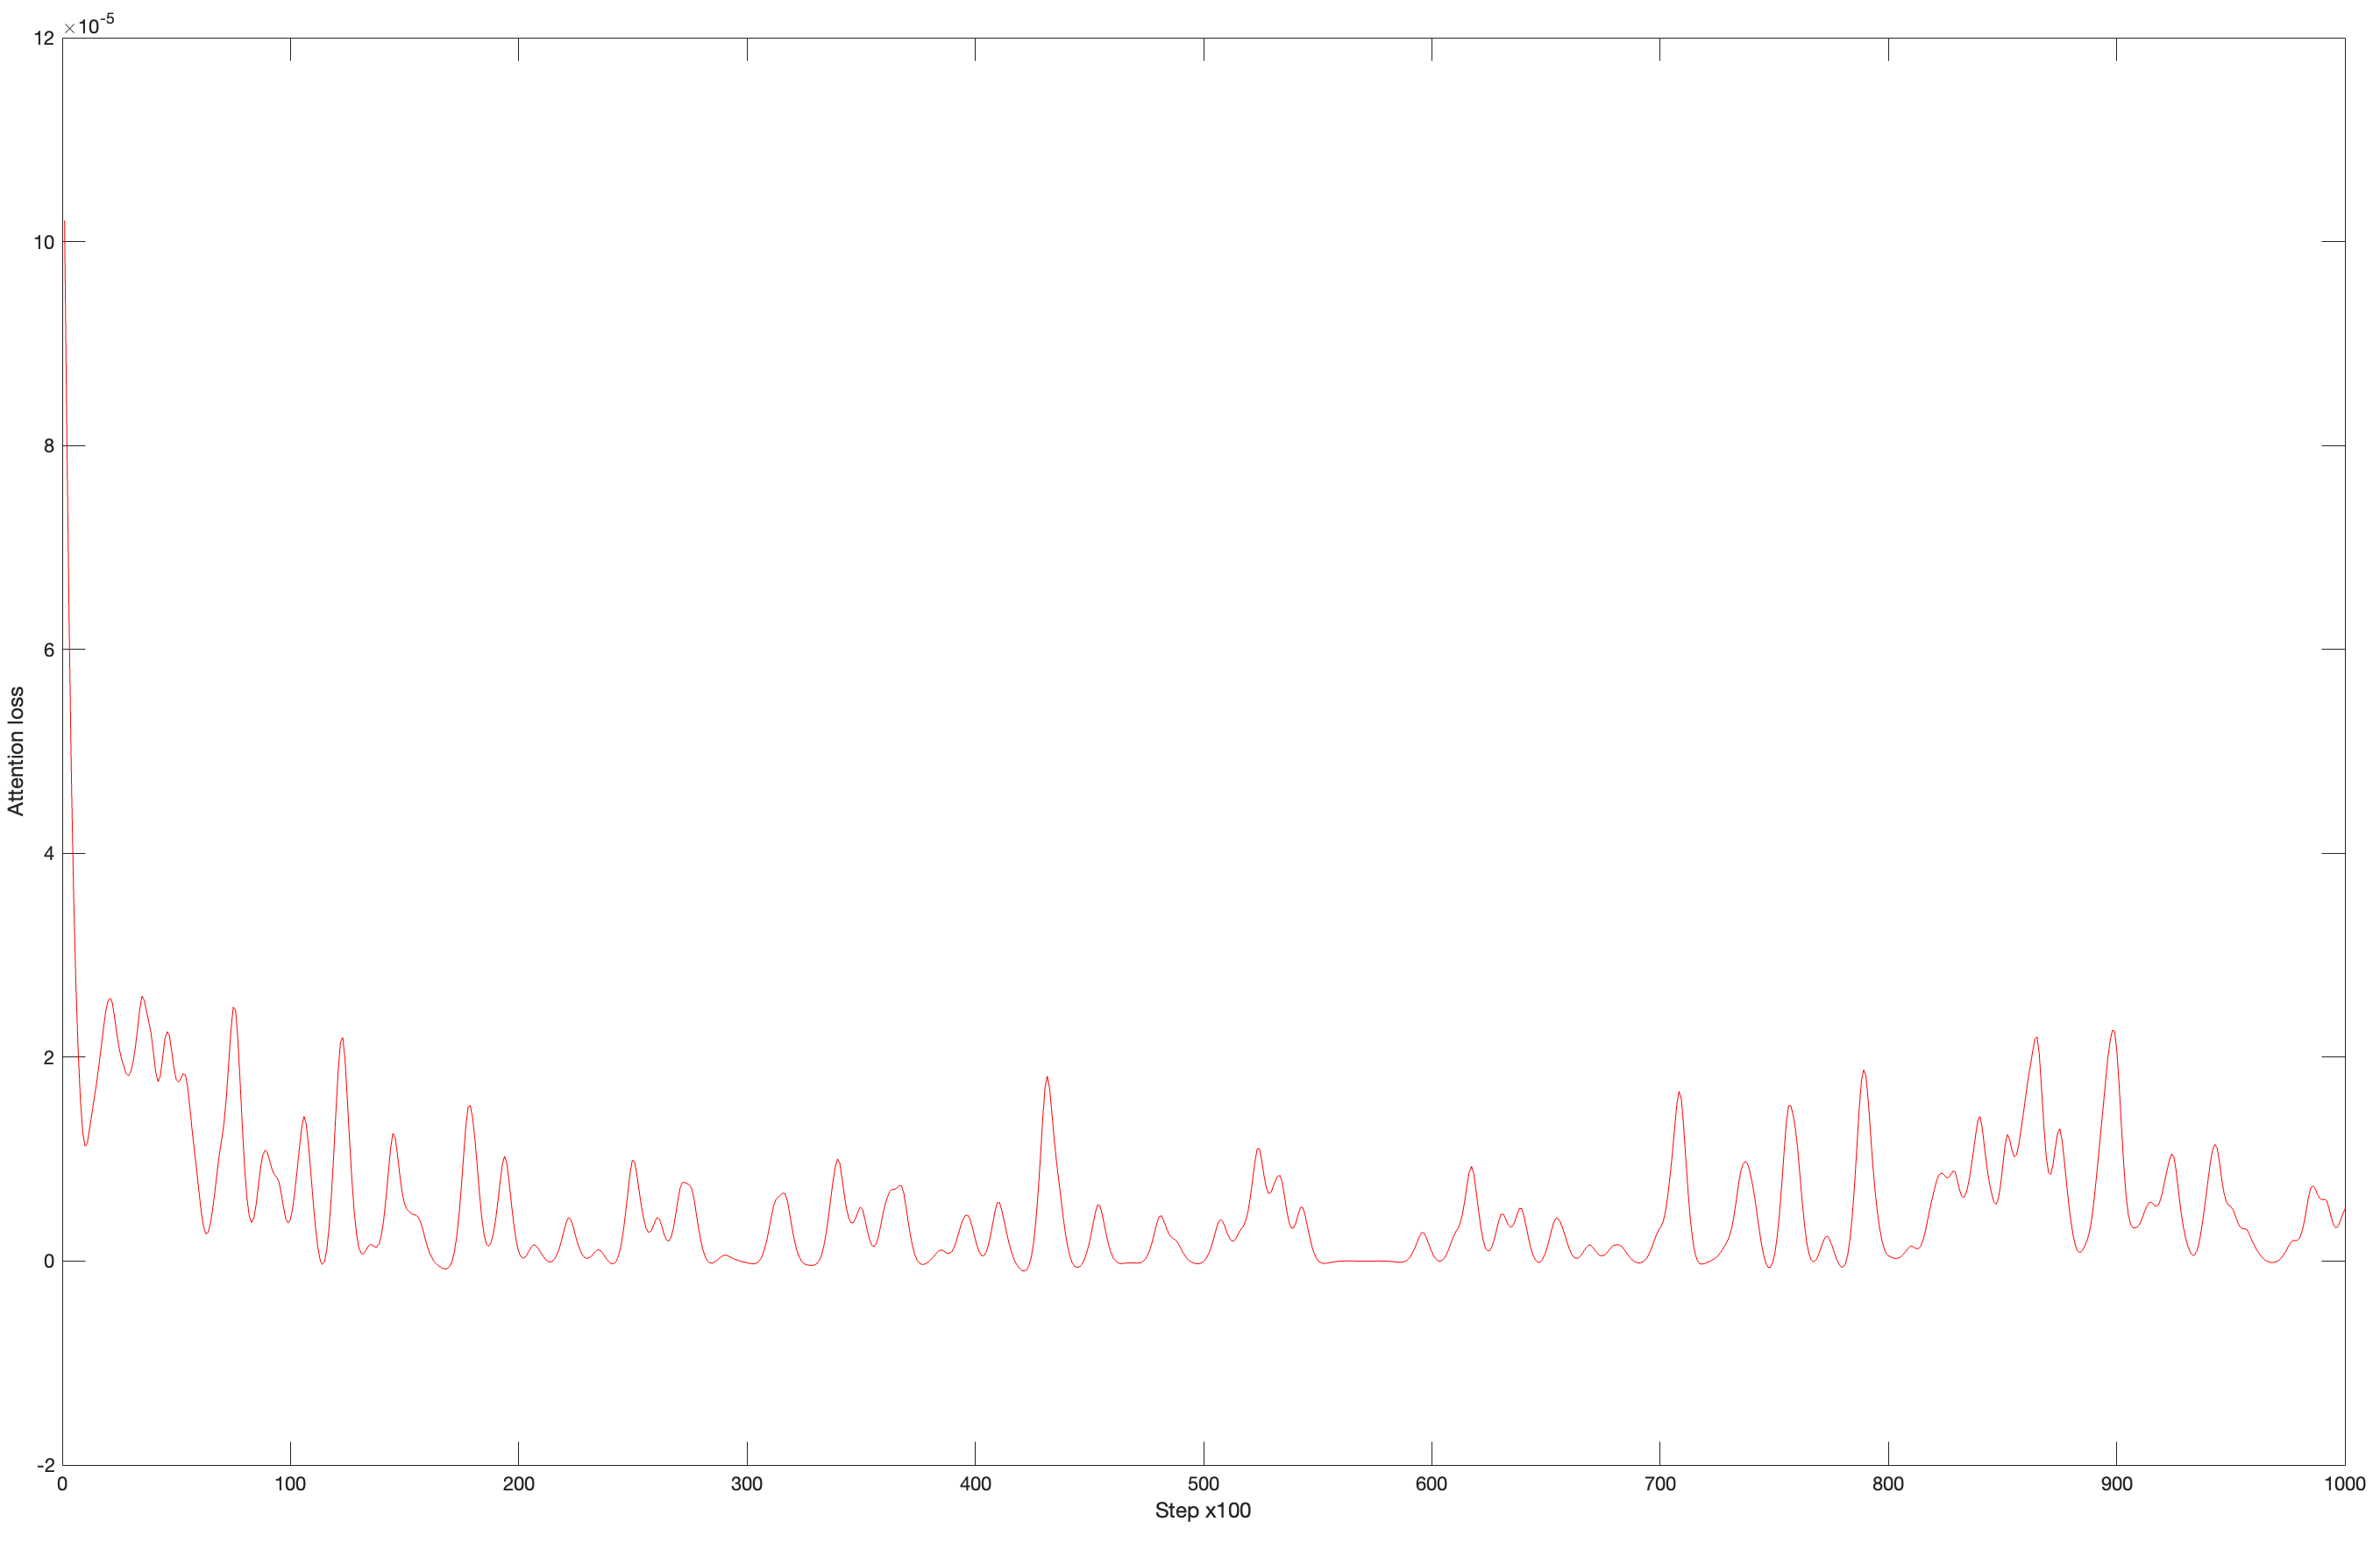
\includegraphics[width=0.9\linewidth]{figures/result/attention_loss}
	\caption[Training result of the Attention Loss]{Training result of the Attention Loss.}
	\label{fig:attention_loss_result}
\end{figure}



\begin{figure}[h!]
	\centering
	\subfigure[train]{
		\begin{minipage}[t]{5cm}
			\centering
			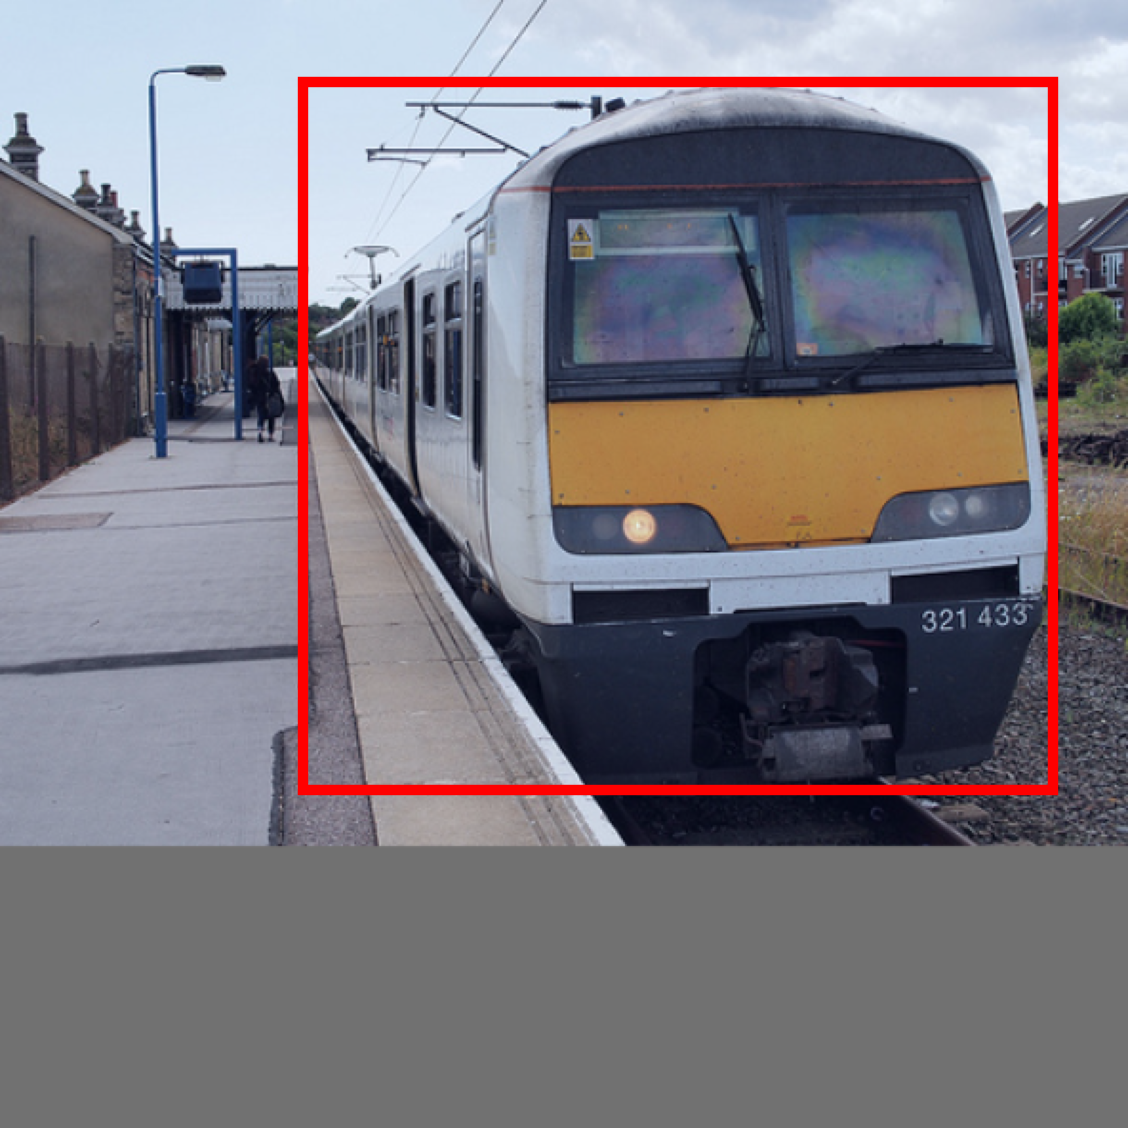
\includegraphics[width=0.9\linewidth]{figures/result/train/obj1}
	\end{minipage}}
	\subfigure[attention map with loss]{
		\begin{minipage}[t]{5cm}
			\centering
			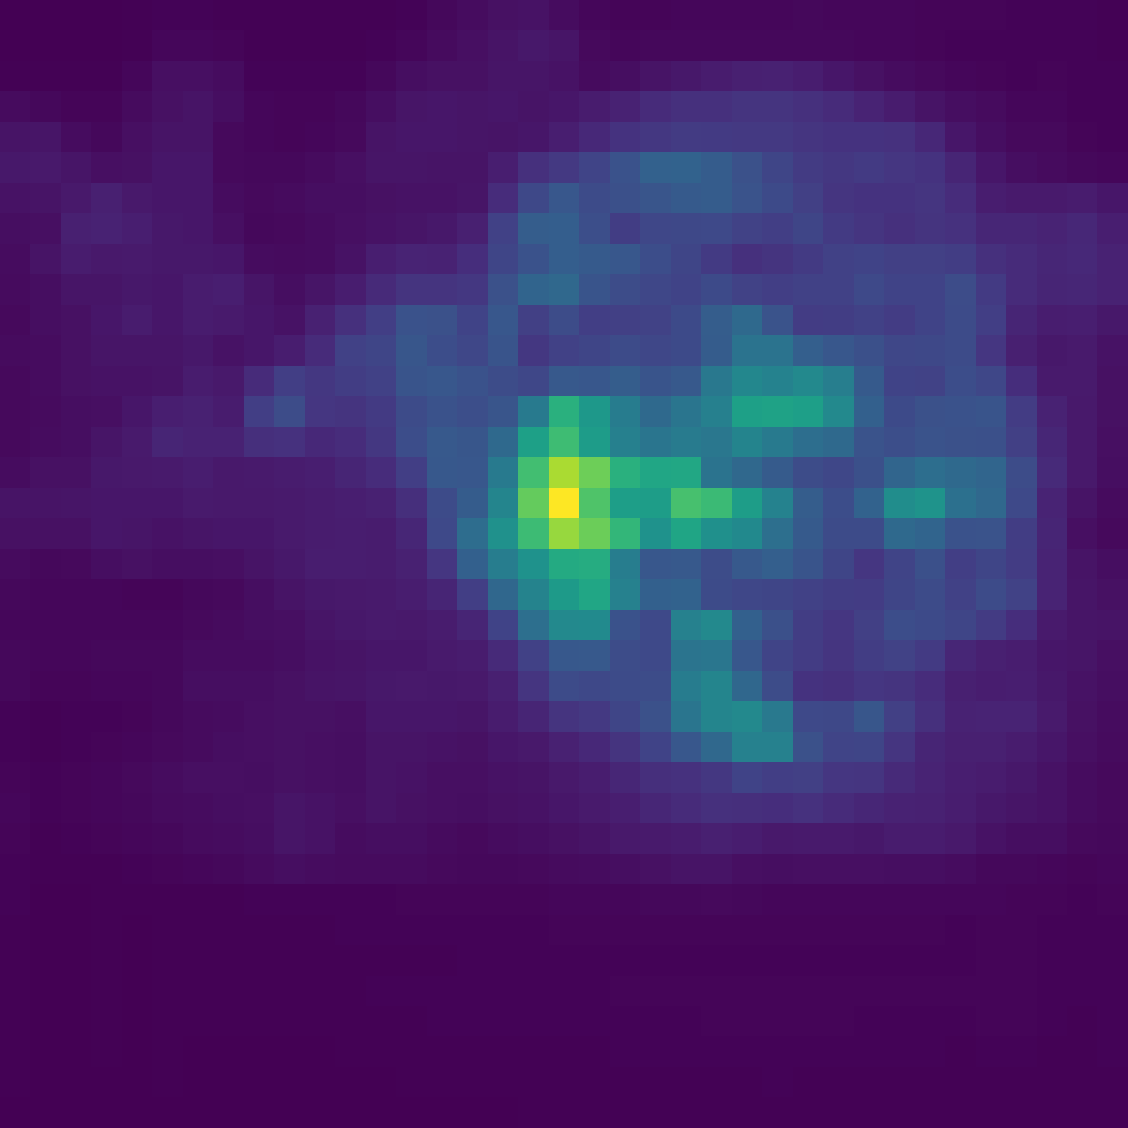
\includegraphics[width=0.9\linewidth]{figures/result/train/att1}
	\end{minipage}}
	\subfigure[ attention map without loss]{
		\begin{minipage}[t]{5cm}
			\centering
			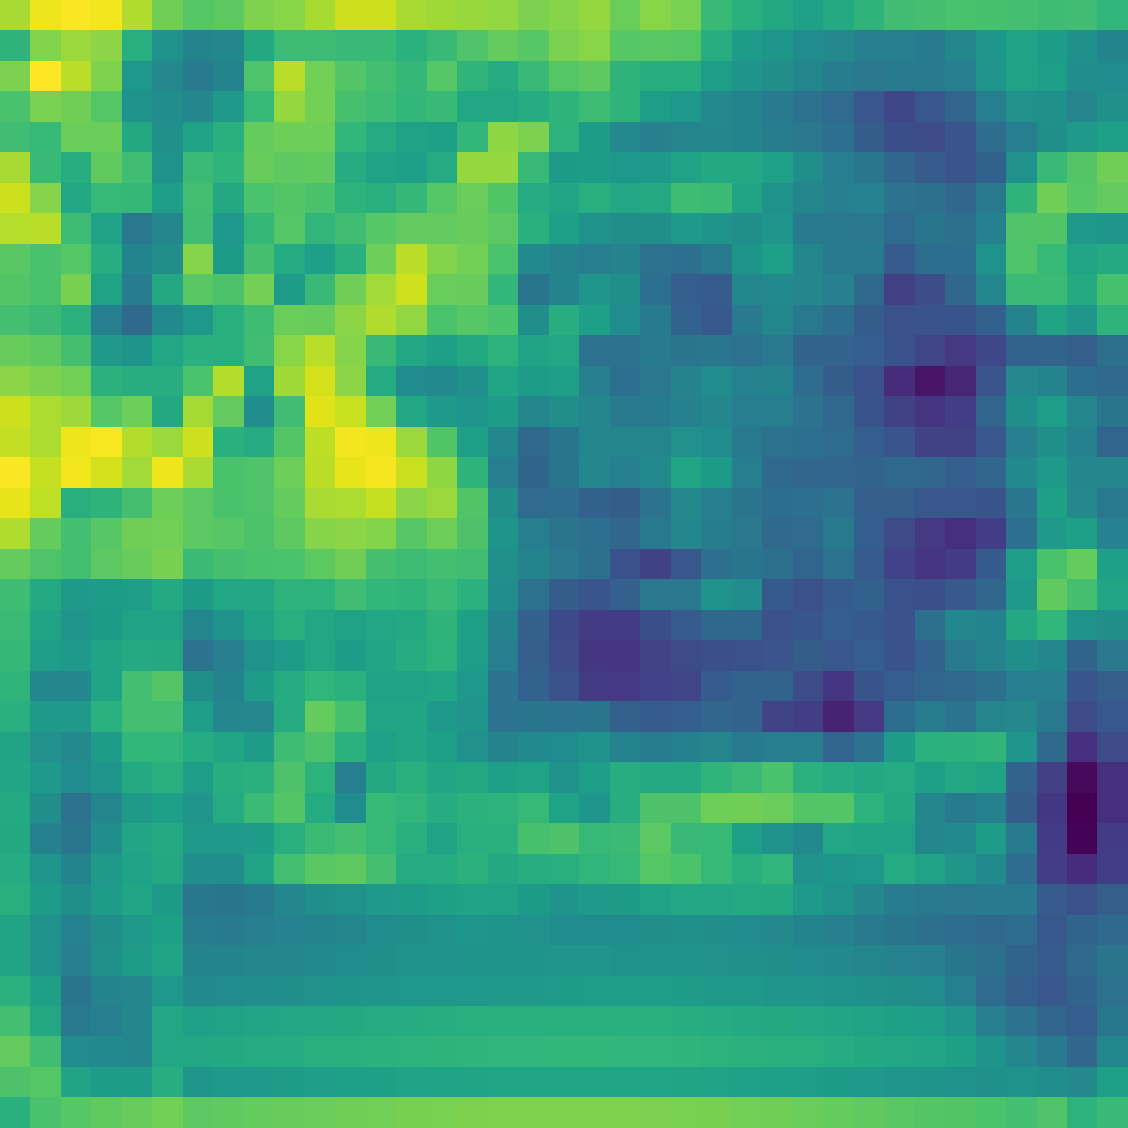
\includegraphics[width=0.9\linewidth]{figures/result/train/no1}
	\end{minipage}}
	
	\subfigure[haus]{
		\begin{minipage}[t]{5cm}
			\centering
			\includegraphics[width=0.9\linewidth]{figures/result/train/obj2}
			\label{fig:motor_man0}
	\end{minipage}}
	\subfigure[attention map with loss]{
		\begin{minipage}[t]{5cm}
			\centering
			\includegraphics[width=0.9\linewidth]{figures/result/train/att2}
			\label{fig:motor_map0}
	\end{minipage}}
	\subfigure[attention map without loss]{
		\begin{minipage}[t]{5cm}
			\centering
			\includegraphics[width=0.9\linewidth]{figures/result/train/no2}
			\label{fig:motor_man1}
	\end{minipage}}

	\subfigure[man]{
		\begin{minipage}[t]{5cm}
			\centering
			\includegraphics[width=0.9\linewidth]{figures/result/train/obj3}
			\label{fig:motor_man0}
	\end{minipage}}
	\subfigure[attention map with loss]{
		\begin{minipage}[t]{5cm}
			\centering
			\includegraphics[width=0.9\linewidth]{figures/result/train/att3}
			\label{fig:motor_map0}
	\end{minipage}}
	\subfigure[attention map without loss]{
		\begin{minipage}[t]{5cm}
			\centering
			\includegraphics[width=0.9\linewidth]{figures/result/train/no3}
			\label{fig:motor_man1}
	\end{minipage}}

	\subfigure[window]{
		\begin{minipage}[t]{5cm}
			\centering
			\includegraphics[width=0.9\linewidth]{figures/result/train/obj4}
			\label{fig:motor_man0}
	\end{minipage}}
	\subfigure[attention map with loss]{
		\begin{minipage}[t]{5cm}
			\centering
			\includegraphics[width=0.9\linewidth]{figures/result/train/att4}
			\label{fig:motor_map0}
	\end{minipage}}
	\subfigure[attention map without loss]{
		\begin{minipage}[t]{5cm}
			\centering
			\includegraphics[width=0.9\linewidth]{figures/result/train/no4}
			\label{fig:motor_man1}
	\end{minipage}}
	
	\caption[The attention map of each pair.]{The attention map of each pair, where $ (a) $ is the ground truth pair and $ (d) $ is its corresponding position in the attention map. $ (b) $, $(c) $ are no relationship pair, and $ (e) $, $ (f) $ is theirs corresponding positions in the attention map.}
	\label{fig:train_attention_loss}
\end{figure}



\begin{figure}[h!]
	\centering
	\subfigure[bus]{
		\begin{minipage}[t]{5cm}
			\centering
			\includegraphics[width=0.9\linewidth]{figures/result/bus/obj1}
	\end{minipage}}
	\subfigure[attention map with loss]{
		\begin{minipage}[t]{5cm}
			\centering
			\includegraphics[width=0.9\linewidth]{figures/result/bus/att1}
	\end{minipage}}
	\subfigure[attention map without loss]{
		\begin{minipage}[t]{5cm}
			\centering
			\includegraphics[width=0.9\linewidth]{figures/result/bus/no1}
	\end{minipage}}
	
	\subfigure[man]{
		\begin{minipage}[t]{5cm}
			\centering
			\includegraphics[width=0.9\linewidth]{figures/result/bus/obj2}
	\end{minipage}}
	\subfigure[attention map with loss]{
		\begin{minipage}[t]{5cm}
			\centering
			\includegraphics[width=0.9\linewidth]{figures/result/bus/att2}
	\end{minipage}}
	\subfigure[attention map without loss]{
		\begin{minipage}[t]{5cm}
			\centering
			\includegraphics[width=0.9\linewidth]{figures/result/bus/no2}
	\end{minipage}}
	
	\subfigure[pants]{
		\begin{minipage}[t]{5cm}
			\centering
			\includegraphics[width=0.9\linewidth]{figures/result/bus/obj3}
	\end{minipage}}
	\subfigure[ attention map with loss]{
		\begin{minipage}[t]{5cm}
			\centering
			\includegraphics[width=0.9\linewidth]{figures/result/bus/att3}
	\end{minipage}}
	\subfigure[ attention map without loss]{
		\begin{minipage}[t]{5cm}
			\centering
			\includegraphics[width=0.9\linewidth]{figures/result/bus/no3}
	\end{minipage}}
	
	\subfigure[board]{
		\begin{minipage}[t]{5cm}
			\centering
			\includegraphics[width=0.9\linewidth]{figures/result/bus/obj4}
	\end{minipage}}
	\subfigure[ attention map with  loss]{
		\begin{minipage}[t]{5cm}
			\centering
			\includegraphics[width=0.9\linewidth]{figures/result/bus/att4}
	\end{minipage}}
	\subfigure[ attention map without  loss]{
		\begin{minipage}[t]{5cm}
			\centering
			\includegraphics[width=0.9\linewidth]{figures/result/bus/no4}
	\end{minipage}}
	
	\caption[The attention map of each pair.]{The attention map of each pair, where $ (a) $ is the ground truth pair and $ (d) $ is its corresponding position in the attention map. $ (b) $, $(c) $ are no relationship pair, and $ (e) $, $ (f) $ is theirs corresponding positions in the attention map.}
	\label{fig:bus}
\end{figure}







\subsection{result}

\begin{table}[!h]
	\centering
	\resizebox{\textwidth}{16mm}{
	\begin{tabular}{c|ccc|ccc|ccc}
		\hline
		\multirow{2}{*}{Models} & \multicolumn{3}{c|}{PredCLS}                                        & \multicolumn{3}{c|}{SGCLS}                                           & \multicolumn{3}{c}{SGDET}                                          \\ \cline{2-10} 
		& R@20 & R@50 & R@100 & R@20 & R@50 & R@100 & R@20 & R@50 & R@100 \\ \hline
		MESSAGE PASSING~\cite{xu2017scene}         & -                    & 44.8                 & 53.1                  & -                    & 21.7                 & 24.4                  & -                    & 3.4                  & 4.2                   \\
		ASSOC EMBED~\cite{newell2017pixels}             & 47.9                 & 54.1                 & 55.4                  & 18.2                 & 21.8                 & 22.6                  & 6.5                  & 8.1                  & 8.2                   \\
		MSDN ~\cite{li2017scene}                   & -                    & 42.3                 & 48.2                  & -                    & 20.9                 & 24.0                  & -                    & 11.7                 & 14.0                  \\
		FREQ ~\cite{zellers2018neural}                   & 53.6                 & 60.6                 & 62.2                  & 29.3                 & 32.3                 & 32.9                  & 20.1                  & 26.2                 & 30.1                  \\
		MotifNet~\cite{zellers2018neural}                & 58.5                 & 65.2                 & 67.1                  & 32.9                 & 35.8                 & 36.5                  & 21.4                 & 27.2                 & 30.3                  \\
		KERN~\cite{chen2019knowledge}                   & -                    & 65.8                 & 67.6                  & -                    & 36.7                 & 37.4                  & -                    & 27.1                 & 29.8                  \\
		RelDN~\cite{zhang2019graphical}                   & 66.9                 & 68.4                 & 68.4                  & 36.1                 & 36.8                 & 36.8                  & 21.1                 & 28.3                 & 32.7                  \\
		Ours                    & 1                    & 1                    & 1                     & 1                    & 1                    & 1                     & 1                    & 1                    & 1                     \\ \hline
	\end{tabular}}

\caption[Comparison with some advanced related works.]{Comparison with some advanced related works. The results of MSDN[21], ASSOC EMBED[34] are obtained from MotifNet[1]. The authors of [1] use their object detector to reimplement for fair comparison. SGRN[20] and our approach also adopt the object detector from [1].}
\label{tab:compare_recall}
\end{table}

\subsection{Visible Results}